% main.tex -- manuscript for Computers & Security (Elsevier), elsarticle; A4 paper.
% Layout (changed 2026-10-06): the journal's own two-column 5p layout, Times, with line numbers for reviewers.
% C&S accepts any layout at first submission ("Your Paper Your Way"); the earlier double-spaced single-column review
% layout is kept in _main_review_layout_backup.tex.
% Build: ./build.sh (compiles supplement, main, supplement, so that cross-references resolve both ways).
% ./build.sh flat makes the single-folder submission bundle (submission/), in which any remaining \todo is an error.
\documentclass[5p,times,twocolumn,authoryear,a4paper]{elsarticle}
% preamble.tex -- shared by main.tex (review build), main_5p.tex (two-column preview) and supplement.tex.
% Before % preamble.tex -- shared by main.tex (review build), main_5p.tex (two-column preview) and supplement.tex.
% Before % preamble.tex -- shared by main.tex (review build), main_5p.tex (two-column preview) and supplement.tex.
% Before \input{preamble}, a document may define
%   \def\SUBMISSION{1}   -- submission build: any remaining \todo stops the compilation with an error.
% Cross-document references (main <-> supplement) use xr-hyper: each document calls \externaldocument after
% \input{preamble}; build.sh compiles the supplement, the main text, then the supplement again. They are written
% \ref*{S:...} / \ref*{M:...} (no hyperlink), because links into the other PDF cannot resolve once Editorial Manager
% merges the files; the flat submission bundle (build.sh flat) replaces them with their resolved numbers.
\usepackage[T1]{fontenc}
\usepackage[utf8]{inputenc}
\usepackage{amsmath,amssymb}
\usepackage{graphicx}
\usepackage{booktabs}
\usepackage{tabularx}
\usepackage{array}
\usepackage[table]{xcolor}
\usepackage{tikz}
\usepackage{xspace}
\usepackage[font=small,labelfont=bf,labelsep=period,justification=justified,singlelinecheck=false]{caption}
\usepackage[hyphens]{xurl}
\usepackage{xr-hyper}
\usepackage[colorlinks=true,allcolors=blue!45!black,breaklinks=true]{hyperref}
% Font expansion off: XeTeX (tectonic, used to build and test) cannot expand fonts, while pdfLaTeX (Editorial Manager)
% would by default, and that would change the line breaks. With protrusion only, both engines break lines the same way.
\usepackage[expansion=false]{microtype}

\graphicspath{{figs/}}

% ---- colours shared with the figures (FIGURE_PLAN.md) ----
\definecolor{ink}{HTML}{0B0B0B}
\definecolor{greyD}{HTML}{52514E}
\definecolor{greyM}{HTML}{8A8984}
\definecolor{accent}{HTML}{D03B3B}

% ---- inline arm markers (same encoding as the figures: shape plus neutral grey) ----
\DeclareRobustCommand{\mkDefault}{\tikz[baseline=-0.55ex]\fill[ink] (0,0) circle (0.85mm);}
\DeclareRobustCommand{\mkDecline}{\tikz[baseline=-0.55ex]\draw[greyD,line width=0.7pt] (-0.75mm,-0.75mm) rectangle (0.75mm,0.75mm);}
\DeclareRobustCommand{\mkGPC}{\tikz[baseline=-0.55ex]\fill[greyM] (-0.95mm,-0.8mm) -- (0.95mm,-0.8mm) -- (0,0.95mm) -- cycle;}
\DeclareRobustCommand{\mkRepeat}{\tikz[baseline=-0.55ex]\draw[greyD,line width=0.7pt] (0,-1mm) -- (1mm,0) -- (0,1mm) -- (-1mm,0) -- cycle;}
% within-arm contrast glyphs (FIGURE_PLAN.md, referee revision): vertical bar = a pixel declaring 'marketing' (Figs 3d, 4a);
% open circle = stores without a banner (Fig 3a); cross = the blocklisted vendor's own pixel (Fig 4a)
\DeclareRobustCommand{\mkBar}{\tikz[baseline=-0.55ex]\draw[ink,line width=0.9pt] (0,-1mm) -- (0,1mm);}
\DeclareRobustCommand{\mkOpen}{\tikz[baseline=-0.55ex]\draw[ink,line width=0.7pt] (0,0) circle (0.8mm);}
\DeclareRobustCommand{\mkCross}{\tikz[baseline=-0.55ex]\draw[ink,line width=0.9pt] (-0.75mm,-0.75mm) -- (0.75mm,0.75mm) (-0.75mm,0.75mm) -- (0.75mm,-0.75mm);}

% ---- text helpers ----
% \code allows a line break after every dot, so long identifiers such as navigator.globalPrivacyControl do not overflow
\DeclareRobustCommand{\code}[1]{\texttt{\codedots{#1}}}
\makeatletter
\def\codedots#1{\@codedots#1.\@nil}
\def\@codedots#1.#2\@nil{#1\ifx\relax#2\relax\else.\allowbreak\@codedots#2\@nil\fi}
\makeatother
\newcommand{\ie}{i.e.,\xspace}
\newcommand{\eg}{e.g.,\xspace}
\newcommand{\RQ}[1]{\textbf{RQ#1}}
% The motivating creator-linked store is pseudonymized as "Store C" until the disclosure of Section 8 is complete
% (final audit, 2026-09-26). Figure 6b carries the same label (figures/scripts/fig6.py).
\newcommand{\storeC}{Store~C\xspace}
% Open items for the authors are printed in red in the review build. In the submission build
% (\def\SUBMISSION{1} before \input{preamble}) every remaining \todo stops the compilation.
\ifdefined\SUBMISSION
  \newcommand{\todo}[1]{\PackageError{manuscript}{Unresolved \string\todo: #1}{Resolve every open item before submission.}}
\else
  \newcommand{\todo}[1]{{\color{accent}[#1]}}
\fi

\setlength{\tabcolsep}{4pt}
\renewcommand{\arraystretch}{1.1}
% Expandable input for generated table bodies (LaTeX's \input breaks \bottomrule inside tabular).
\makeatletter\newcommand{\tabinput}[1]{\@@input #1 }\makeatother
\setlength{\emergencystretch}{3em}
\widowpenalty=10000
\clubpenalty=10000
% ---- float placement: allow tall full-width figures near their first mention ----
\renewcommand{\topfraction}{0.95}
\renewcommand{\dbltopfraction}{0.95}
\renewcommand{\bottomfraction}{0.6}
\renewcommand{\textfraction}{0.05}
\renewcommand{\floatpagefraction}{0.75}
\renewcommand{\dblfloatpagefraction}{0.75}
\setcounter{topnumber}{3}
\setcounter{dbltopnumber}{2}
\setcounter{totalnumber}{5}
\makeatletter
% ---- widefig: a 190 mm figure (Elsevier double-column width) placed at its final printed size and
%      centred on the text block; the graphic may overhang the text block, the caption never does ----
% v2 figures (2026-09-27): when the figure and its full caption are taller than the text block (the single-column
% review build, and the tallest supplementary figures), the float keeps the figure with the caption's bold title and
% the rest of the caption follows as "Figure N (continued)" in a second float right after it. The test is automatic
% (image height + caption height, measured at the caption's width and font); the captions themselves are unchanged
% generated files (captions/*.tex). A caption must start with \textbf{title} to be split; otherwise it is never split.
\newsavebox{\widefigbox}
\newsavebox{\wf@imgbox}
\newsavebox{\wf@capbox}
\newlength{\outertextwidth}
\newif\ifwf@split
\newcommand{\widefigfloat}{figure*}      % float type; the supplement uses figure
\newcommand{\widefigplace}{!tbp}         % default placement of the figure; the supplement uses !htbp
\newcommand{\widefiglegendplace}{!tp}    % placement of the continued legend; the supplement uses !htbp
\newcommand{\wf@ig}[2][]{\sbox{\wf@imgbox}{\wf@includegraphics[#1]{#2}}\usebox{\wf@imgbox}}
\long\def\wf@parse\textbf#1#2\wf@nil{\long\gdef\wf@title{#1}\long\gdef\wf@legend{#2}}
\long\def\wf@starts#1#2\wf@nil{\ifx\textbf#1\global\wf@splittrue\fi}
\long\def\wf@splitcaption#1{%
  \global\wf@splitfalse
  \sbox{\wf@capbox}{\parbox{\outertextwidth}{\small\linespread{1}\selectfont\textbf{Figure S99.}\ #1}}%
  \ifdim\dimexpr\ht\wf@imgbox+\dp\wf@imgbox+\ht\wf@capbox+\dp\wf@capbox+\abovecaptionskip+\belowcaptionskip\relax>\textheight
    \wf@starts#1\relax\wf@nil
  \fi
  \wlog{widefig: image \the\dimexpr\ht\wf@imgbox+\dp\wf@imgbox\relax, caption \the\dimexpr\ht\wf@capbox+\dp\wf@capbox\relax, text height \the\textheight, split \ifwf@split yes\else no\fi}%
  \ifwf@split
    \wf@parse#1\wf@nil
    \begingroup\edef\x{\endgroup\noexpand\wf@caption{\noexpand\textbf{\unexpanded\expandafter{\wf@title}} (The legend continues on the next page.)}}\x
  \else
    \wf@caption{#1}%
  \fi}
\newenvironment{widefig}[1][\widefigplace]
  {\edef\wf@begin{\noexpand\begin{\widefigfloat}[#1]}\edef\wf@end{\noexpand\end{\widefigfloat}}\wf@begin\setlength{\outertextwidth}{\textwidth}%
   \global\wf@splitfalse\sbox{\wf@imgbox}{}%
   \let\wf@includegraphics\includegraphics\let\includegraphics\wf@ig
   \let\wf@caption\caption\let\caption\wf@splitcaption
   \begin{lrbox}{\widefigbox}\begin{minipage}{190mm}\centering\captionsetup{width=\outertextwidth}}
  {\end{minipage}\end{lrbox}\noindent\makebox[\textwidth][c]{\usebox{\widefigbox}}\wf@end
   % (\caption and \includegraphics were changed inside the first float's group, so they are the originals again here)
   \ifwf@split
     \edef\wf@begin{\noexpand\begin{\widefigfloat}[\widefiglegendplace]}\wf@begin
       \caption*{\textbf{Figure~\thefigure\ (continued).}\ \wf@legend}%
     \wf@end
     \global\wf@splitfalse
   \fi}
\makeatother
% ---- single-spaced captions and tables even in the double-spaced review build ----
\captionsetup{font={small,stretch=1}}
\usepackage{etoolbox}
\AtBeginEnvironment{table}{\linespread{1}\selectfont}
\AtBeginEnvironment{table*}{\linespread{1}\selectfont}
\AtBeginEnvironment{figure}{\linespread{1}\selectfont}
\AtBeginEnvironment{figure*}{\linespread{1}\selectfont}
% ---- PDF metadata (the supplement overrides pdftitle) ----
\hypersetup{pdftitle={Consent Enforcement Gaps in Sandboxed Web Pixels: A Large-Scale Measurement of Shopify Storefronts},
  pdfauthor={Devansh Sanghavi},
  pdfkeywords={Web tracking, Consent management platform, Cookie banner, Global Privacy Control, Shopify, Web pixel, Sandboxing, Web measurement}}
, a document may define
%   \def\SUBMISSION{1}   -- submission build: any remaining \todo stops the compilation with an error.
% Cross-document references (main <-> supplement) use xr-hyper: each document calls \externaldocument after
% % preamble.tex -- shared by main.tex (review build), main_5p.tex (two-column preview) and supplement.tex.
% Before \input{preamble}, a document may define
%   \def\SUBMISSION{1}   -- submission build: any remaining \todo stops the compilation with an error.
% Cross-document references (main <-> supplement) use xr-hyper: each document calls \externaldocument after
% \input{preamble}; build.sh compiles the supplement, the main text, then the supplement again. They are written
% \ref*{S:...} / \ref*{M:...} (no hyperlink), because links into the other PDF cannot resolve once Editorial Manager
% merges the files; the flat submission bundle (build.sh flat) replaces them with their resolved numbers.
\usepackage[T1]{fontenc}
\usepackage[utf8]{inputenc}
\usepackage{amsmath,amssymb}
\usepackage{graphicx}
\usepackage{booktabs}
\usepackage{tabularx}
\usepackage{array}
\usepackage[table]{xcolor}
\usepackage{tikz}
\usepackage{xspace}
\usepackage[font=small,labelfont=bf,labelsep=period,justification=justified,singlelinecheck=false]{caption}
\usepackage[hyphens]{xurl}
\usepackage{xr-hyper}
\usepackage[colorlinks=true,allcolors=blue!45!black,breaklinks=true]{hyperref}
% Font expansion off: XeTeX (tectonic, used to build and test) cannot expand fonts, while pdfLaTeX (Editorial Manager)
% would by default, and that would change the line breaks. With protrusion only, both engines break lines the same way.
\usepackage[expansion=false]{microtype}

\graphicspath{{figs/}}

% ---- colours shared with the figures (FIGURE_PLAN.md) ----
\definecolor{ink}{HTML}{0B0B0B}
\definecolor{greyD}{HTML}{52514E}
\definecolor{greyM}{HTML}{8A8984}
\definecolor{accent}{HTML}{D03B3B}

% ---- inline arm markers (same encoding as the figures: shape plus neutral grey) ----
\DeclareRobustCommand{\mkDefault}{\tikz[baseline=-0.55ex]\fill[ink] (0,0) circle (0.85mm);}
\DeclareRobustCommand{\mkDecline}{\tikz[baseline=-0.55ex]\draw[greyD,line width=0.7pt] (-0.75mm,-0.75mm) rectangle (0.75mm,0.75mm);}
\DeclareRobustCommand{\mkGPC}{\tikz[baseline=-0.55ex]\fill[greyM] (-0.95mm,-0.8mm) -- (0.95mm,-0.8mm) -- (0,0.95mm) -- cycle;}
\DeclareRobustCommand{\mkRepeat}{\tikz[baseline=-0.55ex]\draw[greyD,line width=0.7pt] (0,-1mm) -- (1mm,0) -- (0,1mm) -- (-1mm,0) -- cycle;}
% within-arm contrast glyphs (FIGURE_PLAN.md, referee revision): vertical bar = a pixel declaring 'marketing' (Figs 3d, 4a);
% open circle = stores without a banner (Fig 3a); cross = the blocklisted vendor's own pixel (Fig 4a)
\DeclareRobustCommand{\mkBar}{\tikz[baseline=-0.55ex]\draw[ink,line width=0.9pt] (0,-1mm) -- (0,1mm);}
\DeclareRobustCommand{\mkOpen}{\tikz[baseline=-0.55ex]\draw[ink,line width=0.7pt] (0,0) circle (0.8mm);}
\DeclareRobustCommand{\mkCross}{\tikz[baseline=-0.55ex]\draw[ink,line width=0.9pt] (-0.75mm,-0.75mm) -- (0.75mm,0.75mm) (-0.75mm,0.75mm) -- (0.75mm,-0.75mm);}

% ---- text helpers ----
% \code allows a line break after every dot, so long identifiers such as navigator.globalPrivacyControl do not overflow
\DeclareRobustCommand{\code}[1]{\texttt{\codedots{#1}}}
\makeatletter
\def\codedots#1{\@codedots#1.\@nil}
\def\@codedots#1.#2\@nil{#1\ifx\relax#2\relax\else.\allowbreak\@codedots#2\@nil\fi}
\makeatother
\newcommand{\ie}{i.e.,\xspace}
\newcommand{\eg}{e.g.,\xspace}
\newcommand{\RQ}[1]{\textbf{RQ#1}}
% The motivating creator-linked store is pseudonymized as "Store C" until the disclosure of Section 8 is complete
% (final audit, 2026-09-26). Figure 6b carries the same label (figures/scripts/fig6.py).
\newcommand{\storeC}{Store~C\xspace}
% Open items for the authors are printed in red in the review build. In the submission build
% (\def\SUBMISSION{1} before \input{preamble}) every remaining \todo stops the compilation.
\ifdefined\SUBMISSION
  \newcommand{\todo}[1]{\PackageError{manuscript}{Unresolved \string\todo: #1}{Resolve every open item before submission.}}
\else
  \newcommand{\todo}[1]{{\color{accent}[#1]}}
\fi

\setlength{\tabcolsep}{4pt}
\renewcommand{\arraystretch}{1.1}
% Expandable input for generated table bodies (LaTeX's \input breaks \bottomrule inside tabular).
\makeatletter\newcommand{\tabinput}[1]{\@@input #1 }\makeatother
\setlength{\emergencystretch}{3em}
\widowpenalty=10000
\clubpenalty=10000
% ---- float placement: allow tall full-width figures near their first mention ----
\renewcommand{\topfraction}{0.95}
\renewcommand{\dbltopfraction}{0.95}
\renewcommand{\bottomfraction}{0.6}
\renewcommand{\textfraction}{0.05}
\renewcommand{\floatpagefraction}{0.75}
\renewcommand{\dblfloatpagefraction}{0.75}
\setcounter{topnumber}{3}
\setcounter{dbltopnumber}{2}
\setcounter{totalnumber}{5}
\makeatletter
% ---- widefig: a 190 mm figure (Elsevier double-column width) placed at its final printed size and
%      centred on the text block; the graphic may overhang the text block, the caption never does ----
% v2 figures (2026-09-27): when the figure and its full caption are taller than the text block (the single-column
% review build, and the tallest supplementary figures), the float keeps the figure with the caption's bold title and
% the rest of the caption follows as "Figure N (continued)" in a second float right after it. The test is automatic
% (image height + caption height, measured at the caption's width and font); the captions themselves are unchanged
% generated files (captions/*.tex). A caption must start with \textbf{title} to be split; otherwise it is never split.
\newsavebox{\widefigbox}
\newsavebox{\wf@imgbox}
\newsavebox{\wf@capbox}
\newlength{\outertextwidth}
\newif\ifwf@split
\newcommand{\widefigfloat}{figure*}      % float type; the supplement uses figure
\newcommand{\widefigplace}{!tbp}         % default placement of the figure; the supplement uses !htbp
\newcommand{\widefiglegendplace}{!tp}    % placement of the continued legend; the supplement uses !htbp
\newcommand{\wf@ig}[2][]{\sbox{\wf@imgbox}{\wf@includegraphics[#1]{#2}}\usebox{\wf@imgbox}}
\long\def\wf@parse\textbf#1#2\wf@nil{\long\gdef\wf@title{#1}\long\gdef\wf@legend{#2}}
\long\def\wf@starts#1#2\wf@nil{\ifx\textbf#1\global\wf@splittrue\fi}
\long\def\wf@splitcaption#1{%
  \global\wf@splitfalse
  \sbox{\wf@capbox}{\parbox{\outertextwidth}{\small\linespread{1}\selectfont\textbf{Figure S99.}\ #1}}%
  \ifdim\dimexpr\ht\wf@imgbox+\dp\wf@imgbox+\ht\wf@capbox+\dp\wf@capbox+\abovecaptionskip+\belowcaptionskip\relax>\textheight
    \wf@starts#1\relax\wf@nil
  \fi
  \wlog{widefig: image \the\dimexpr\ht\wf@imgbox+\dp\wf@imgbox\relax, caption \the\dimexpr\ht\wf@capbox+\dp\wf@capbox\relax, text height \the\textheight, split \ifwf@split yes\else no\fi}%
  \ifwf@split
    \wf@parse#1\wf@nil
    \begingroup\edef\x{\endgroup\noexpand\wf@caption{\noexpand\textbf{\unexpanded\expandafter{\wf@title}} (The legend continues on the next page.)}}\x
  \else
    \wf@caption{#1}%
  \fi}
\newenvironment{widefig}[1][\widefigplace]
  {\edef\wf@begin{\noexpand\begin{\widefigfloat}[#1]}\edef\wf@end{\noexpand\end{\widefigfloat}}\wf@begin\setlength{\outertextwidth}{\textwidth}%
   \global\wf@splitfalse\sbox{\wf@imgbox}{}%
   \let\wf@includegraphics\includegraphics\let\includegraphics\wf@ig
   \let\wf@caption\caption\let\caption\wf@splitcaption
   \begin{lrbox}{\widefigbox}\begin{minipage}{190mm}\centering\captionsetup{width=\outertextwidth}}
  {\end{minipage}\end{lrbox}\noindent\makebox[\textwidth][c]{\usebox{\widefigbox}}\wf@end
   % (\caption and \includegraphics were changed inside the first float's group, so they are the originals again here)
   \ifwf@split
     \edef\wf@begin{\noexpand\begin{\widefigfloat}[\widefiglegendplace]}\wf@begin
       \caption*{\textbf{Figure~\thefigure\ (continued).}\ \wf@legend}%
     \wf@end
     \global\wf@splitfalse
   \fi}
\makeatother
% ---- single-spaced captions and tables even in the double-spaced review build ----
\captionsetup{font={small,stretch=1}}
\usepackage{etoolbox}
\AtBeginEnvironment{table}{\linespread{1}\selectfont}
\AtBeginEnvironment{table*}{\linespread{1}\selectfont}
\AtBeginEnvironment{figure}{\linespread{1}\selectfont}
\AtBeginEnvironment{figure*}{\linespread{1}\selectfont}
% ---- PDF metadata (the supplement overrides pdftitle) ----
\hypersetup{pdftitle={Consent Enforcement Gaps in Sandboxed Web Pixels: A Large-Scale Measurement of Shopify Storefronts},
  pdfauthor={Devansh Sanghavi},
  pdfkeywords={Web tracking, Consent management platform, Cookie banner, Global Privacy Control, Shopify, Web pixel, Sandboxing, Web measurement}}
; build.sh compiles the supplement, the main text, then the supplement again. They are written
% \ref*{S:...} / \ref*{M:...} (no hyperlink), because links into the other PDF cannot resolve once Editorial Manager
% merges the files; the flat submission bundle (build.sh flat) replaces them with their resolved numbers.
\usepackage[T1]{fontenc}
\usepackage[utf8]{inputenc}
\usepackage{amsmath,amssymb}
\usepackage{graphicx}
\usepackage{booktabs}
\usepackage{tabularx}
\usepackage{array}
\usepackage[table]{xcolor}
\usepackage{tikz}
\usepackage{xspace}
\usepackage[font=small,labelfont=bf,labelsep=period,justification=justified,singlelinecheck=false]{caption}
\usepackage[hyphens]{xurl}
\usepackage{xr-hyper}
\usepackage[colorlinks=true,allcolors=blue!45!black,breaklinks=true]{hyperref}
% Font expansion off: XeTeX (tectonic, used to build and test) cannot expand fonts, while pdfLaTeX (Editorial Manager)
% would by default, and that would change the line breaks. With protrusion only, both engines break lines the same way.
\usepackage[expansion=false]{microtype}

\graphicspath{{figs/}}

% ---- colours shared with the figures (FIGURE_PLAN.md) ----
\definecolor{ink}{HTML}{0B0B0B}
\definecolor{greyD}{HTML}{52514E}
\definecolor{greyM}{HTML}{8A8984}
\definecolor{accent}{HTML}{D03B3B}

% ---- inline arm markers (same encoding as the figures: shape plus neutral grey) ----
\DeclareRobustCommand{\mkDefault}{\tikz[baseline=-0.55ex]\fill[ink] (0,0) circle (0.85mm);}
\DeclareRobustCommand{\mkDecline}{\tikz[baseline=-0.55ex]\draw[greyD,line width=0.7pt] (-0.75mm,-0.75mm) rectangle (0.75mm,0.75mm);}
\DeclareRobustCommand{\mkGPC}{\tikz[baseline=-0.55ex]\fill[greyM] (-0.95mm,-0.8mm) -- (0.95mm,-0.8mm) -- (0,0.95mm) -- cycle;}
\DeclareRobustCommand{\mkRepeat}{\tikz[baseline=-0.55ex]\draw[greyD,line width=0.7pt] (0,-1mm) -- (1mm,0) -- (0,1mm) -- (-1mm,0) -- cycle;}
% within-arm contrast glyphs (FIGURE_PLAN.md, referee revision): vertical bar = a pixel declaring 'marketing' (Figs 3d, 4a);
% open circle = stores without a banner (Fig 3a); cross = the blocklisted vendor's own pixel (Fig 4a)
\DeclareRobustCommand{\mkBar}{\tikz[baseline=-0.55ex]\draw[ink,line width=0.9pt] (0,-1mm) -- (0,1mm);}
\DeclareRobustCommand{\mkOpen}{\tikz[baseline=-0.55ex]\draw[ink,line width=0.7pt] (0,0) circle (0.8mm);}
\DeclareRobustCommand{\mkCross}{\tikz[baseline=-0.55ex]\draw[ink,line width=0.9pt] (-0.75mm,-0.75mm) -- (0.75mm,0.75mm) (-0.75mm,0.75mm) -- (0.75mm,-0.75mm);}

% ---- text helpers ----
% \code allows a line break after every dot, so long identifiers such as navigator.globalPrivacyControl do not overflow
\DeclareRobustCommand{\code}[1]{\texttt{\codedots{#1}}}
\makeatletter
\def\codedots#1{\@codedots#1.\@nil}
\def\@codedots#1.#2\@nil{#1\ifx\relax#2\relax\else.\allowbreak\@codedots#2\@nil\fi}
\makeatother
\newcommand{\ie}{i.e.,\xspace}
\newcommand{\eg}{e.g.,\xspace}
\newcommand{\RQ}[1]{\textbf{RQ#1}}
% The motivating creator-linked store is pseudonymized as "Store C" until the disclosure of Section 8 is complete
% (final audit, 2026-09-26). Figure 6b carries the same label (figures/scripts/fig6.py).
\newcommand{\storeC}{Store~C\xspace}
% Open items for the authors are printed in red in the review build. In the submission build
% (\def\SUBMISSION{1} before % preamble.tex -- shared by main.tex (review build), main_5p.tex (two-column preview) and supplement.tex.
% Before \input{preamble}, a document may define
%   \def\SUBMISSION{1}   -- submission build: any remaining \todo stops the compilation with an error.
% Cross-document references (main <-> supplement) use xr-hyper: each document calls \externaldocument after
% \input{preamble}; build.sh compiles the supplement, the main text, then the supplement again. They are written
% \ref*{S:...} / \ref*{M:...} (no hyperlink), because links into the other PDF cannot resolve once Editorial Manager
% merges the files; the flat submission bundle (build.sh flat) replaces them with their resolved numbers.
\usepackage[T1]{fontenc}
\usepackage[utf8]{inputenc}
\usepackage{amsmath,amssymb}
\usepackage{graphicx}
\usepackage{booktabs}
\usepackage{tabularx}
\usepackage{array}
\usepackage[table]{xcolor}
\usepackage{tikz}
\usepackage{xspace}
\usepackage[font=small,labelfont=bf,labelsep=period,justification=justified,singlelinecheck=false]{caption}
\usepackage[hyphens]{xurl}
\usepackage{xr-hyper}
\usepackage[colorlinks=true,allcolors=blue!45!black,breaklinks=true]{hyperref}
% Font expansion off: XeTeX (tectonic, used to build and test) cannot expand fonts, while pdfLaTeX (Editorial Manager)
% would by default, and that would change the line breaks. With protrusion only, both engines break lines the same way.
\usepackage[expansion=false]{microtype}

\graphicspath{{figs/}}

% ---- colours shared with the figures (FIGURE_PLAN.md) ----
\definecolor{ink}{HTML}{0B0B0B}
\definecolor{greyD}{HTML}{52514E}
\definecolor{greyM}{HTML}{8A8984}
\definecolor{accent}{HTML}{D03B3B}

% ---- inline arm markers (same encoding as the figures: shape plus neutral grey) ----
\DeclareRobustCommand{\mkDefault}{\tikz[baseline=-0.55ex]\fill[ink] (0,0) circle (0.85mm);}
\DeclareRobustCommand{\mkDecline}{\tikz[baseline=-0.55ex]\draw[greyD,line width=0.7pt] (-0.75mm,-0.75mm) rectangle (0.75mm,0.75mm);}
\DeclareRobustCommand{\mkGPC}{\tikz[baseline=-0.55ex]\fill[greyM] (-0.95mm,-0.8mm) -- (0.95mm,-0.8mm) -- (0,0.95mm) -- cycle;}
\DeclareRobustCommand{\mkRepeat}{\tikz[baseline=-0.55ex]\draw[greyD,line width=0.7pt] (0,-1mm) -- (1mm,0) -- (0,1mm) -- (-1mm,0) -- cycle;}
% within-arm contrast glyphs (FIGURE_PLAN.md, referee revision): vertical bar = a pixel declaring 'marketing' (Figs 3d, 4a);
% open circle = stores without a banner (Fig 3a); cross = the blocklisted vendor's own pixel (Fig 4a)
\DeclareRobustCommand{\mkBar}{\tikz[baseline=-0.55ex]\draw[ink,line width=0.9pt] (0,-1mm) -- (0,1mm);}
\DeclareRobustCommand{\mkOpen}{\tikz[baseline=-0.55ex]\draw[ink,line width=0.7pt] (0,0) circle (0.8mm);}
\DeclareRobustCommand{\mkCross}{\tikz[baseline=-0.55ex]\draw[ink,line width=0.9pt] (-0.75mm,-0.75mm) -- (0.75mm,0.75mm) (-0.75mm,0.75mm) -- (0.75mm,-0.75mm);}

% ---- text helpers ----
% \code allows a line break after every dot, so long identifiers such as navigator.globalPrivacyControl do not overflow
\DeclareRobustCommand{\code}[1]{\texttt{\codedots{#1}}}
\makeatletter
\def\codedots#1{\@codedots#1.\@nil}
\def\@codedots#1.#2\@nil{#1\ifx\relax#2\relax\else.\allowbreak\@codedots#2\@nil\fi}
\makeatother
\newcommand{\ie}{i.e.,\xspace}
\newcommand{\eg}{e.g.,\xspace}
\newcommand{\RQ}[1]{\textbf{RQ#1}}
% The motivating creator-linked store is pseudonymized as "Store C" until the disclosure of Section 8 is complete
% (final audit, 2026-09-26). Figure 6b carries the same label (figures/scripts/fig6.py).
\newcommand{\storeC}{Store~C\xspace}
% Open items for the authors are printed in red in the review build. In the submission build
% (\def\SUBMISSION{1} before \input{preamble}) every remaining \todo stops the compilation.
\ifdefined\SUBMISSION
  \newcommand{\todo}[1]{\PackageError{manuscript}{Unresolved \string\todo: #1}{Resolve every open item before submission.}}
\else
  \newcommand{\todo}[1]{{\color{accent}[#1]}}
\fi

\setlength{\tabcolsep}{4pt}
\renewcommand{\arraystretch}{1.1}
% Expandable input for generated table bodies (LaTeX's \input breaks \bottomrule inside tabular).
\makeatletter\newcommand{\tabinput}[1]{\@@input #1 }\makeatother
\setlength{\emergencystretch}{3em}
\widowpenalty=10000
\clubpenalty=10000
% ---- float placement: allow tall full-width figures near their first mention ----
\renewcommand{\topfraction}{0.95}
\renewcommand{\dbltopfraction}{0.95}
\renewcommand{\bottomfraction}{0.6}
\renewcommand{\textfraction}{0.05}
\renewcommand{\floatpagefraction}{0.75}
\renewcommand{\dblfloatpagefraction}{0.75}
\setcounter{topnumber}{3}
\setcounter{dbltopnumber}{2}
\setcounter{totalnumber}{5}
\makeatletter
% ---- widefig: a 190 mm figure (Elsevier double-column width) placed at its final printed size and
%      centred on the text block; the graphic may overhang the text block, the caption never does ----
% v2 figures (2026-09-27): when the figure and its full caption are taller than the text block (the single-column
% review build, and the tallest supplementary figures), the float keeps the figure with the caption's bold title and
% the rest of the caption follows as "Figure N (continued)" in a second float right after it. The test is automatic
% (image height + caption height, measured at the caption's width and font); the captions themselves are unchanged
% generated files (captions/*.tex). A caption must start with \textbf{title} to be split; otherwise it is never split.
\newsavebox{\widefigbox}
\newsavebox{\wf@imgbox}
\newsavebox{\wf@capbox}
\newlength{\outertextwidth}
\newif\ifwf@split
\newcommand{\widefigfloat}{figure*}      % float type; the supplement uses figure
\newcommand{\widefigplace}{!tbp}         % default placement of the figure; the supplement uses !htbp
\newcommand{\widefiglegendplace}{!tp}    % placement of the continued legend; the supplement uses !htbp
\newcommand{\wf@ig}[2][]{\sbox{\wf@imgbox}{\wf@includegraphics[#1]{#2}}\usebox{\wf@imgbox}}
\long\def\wf@parse\textbf#1#2\wf@nil{\long\gdef\wf@title{#1}\long\gdef\wf@legend{#2}}
\long\def\wf@starts#1#2\wf@nil{\ifx\textbf#1\global\wf@splittrue\fi}
\long\def\wf@splitcaption#1{%
  \global\wf@splitfalse
  \sbox{\wf@capbox}{\parbox{\outertextwidth}{\small\linespread{1}\selectfont\textbf{Figure S99.}\ #1}}%
  \ifdim\dimexpr\ht\wf@imgbox+\dp\wf@imgbox+\ht\wf@capbox+\dp\wf@capbox+\abovecaptionskip+\belowcaptionskip\relax>\textheight
    \wf@starts#1\relax\wf@nil
  \fi
  \wlog{widefig: image \the\dimexpr\ht\wf@imgbox+\dp\wf@imgbox\relax, caption \the\dimexpr\ht\wf@capbox+\dp\wf@capbox\relax, text height \the\textheight, split \ifwf@split yes\else no\fi}%
  \ifwf@split
    \wf@parse#1\wf@nil
    \begingroup\edef\x{\endgroup\noexpand\wf@caption{\noexpand\textbf{\unexpanded\expandafter{\wf@title}} (The legend continues on the next page.)}}\x
  \else
    \wf@caption{#1}%
  \fi}
\newenvironment{widefig}[1][\widefigplace]
  {\edef\wf@begin{\noexpand\begin{\widefigfloat}[#1]}\edef\wf@end{\noexpand\end{\widefigfloat}}\wf@begin\setlength{\outertextwidth}{\textwidth}%
   \global\wf@splitfalse\sbox{\wf@imgbox}{}%
   \let\wf@includegraphics\includegraphics\let\includegraphics\wf@ig
   \let\wf@caption\caption\let\caption\wf@splitcaption
   \begin{lrbox}{\widefigbox}\begin{minipage}{190mm}\centering\captionsetup{width=\outertextwidth}}
  {\end{minipage}\end{lrbox}\noindent\makebox[\textwidth][c]{\usebox{\widefigbox}}\wf@end
   % (\caption and \includegraphics were changed inside the first float's group, so they are the originals again here)
   \ifwf@split
     \edef\wf@begin{\noexpand\begin{\widefigfloat}[\widefiglegendplace]}\wf@begin
       \caption*{\textbf{Figure~\thefigure\ (continued).}\ \wf@legend}%
     \wf@end
     \global\wf@splitfalse
   \fi}
\makeatother
% ---- single-spaced captions and tables even in the double-spaced review build ----
\captionsetup{font={small,stretch=1}}
\usepackage{etoolbox}
\AtBeginEnvironment{table}{\linespread{1}\selectfont}
\AtBeginEnvironment{table*}{\linespread{1}\selectfont}
\AtBeginEnvironment{figure}{\linespread{1}\selectfont}
\AtBeginEnvironment{figure*}{\linespread{1}\selectfont}
% ---- PDF metadata (the supplement overrides pdftitle) ----
\hypersetup{pdftitle={Consent Enforcement Gaps in Sandboxed Web Pixels: A Large-Scale Measurement of Shopify Storefronts},
  pdfauthor={Devansh Sanghavi},
  pdfkeywords={Web tracking, Consent management platform, Cookie banner, Global Privacy Control, Shopify, Web pixel, Sandboxing, Web measurement}}
) every remaining \todo stops the compilation.
\ifdefined\SUBMISSION
  \newcommand{\todo}[1]{\PackageError{manuscript}{Unresolved \string\todo: #1}{Resolve every open item before submission.}}
\else
  \newcommand{\todo}[1]{{\color{accent}[#1]}}
\fi

\setlength{\tabcolsep}{4pt}
\renewcommand{\arraystretch}{1.1}
% Expandable input for generated table bodies (LaTeX's \input breaks \bottomrule inside tabular).
\makeatletter\newcommand{\tabinput}[1]{\@@input #1 }\makeatother
\setlength{\emergencystretch}{3em}
\widowpenalty=10000
\clubpenalty=10000
% ---- float placement: allow tall full-width figures near their first mention ----
\renewcommand{\topfraction}{0.95}
\renewcommand{\dbltopfraction}{0.95}
\renewcommand{\bottomfraction}{0.6}
\renewcommand{\textfraction}{0.05}
\renewcommand{\floatpagefraction}{0.75}
\renewcommand{\dblfloatpagefraction}{0.75}
\setcounter{topnumber}{3}
\setcounter{dbltopnumber}{2}
\setcounter{totalnumber}{5}
\makeatletter
% ---- widefig: a 190 mm figure (Elsevier double-column width) placed at its final printed size and
%      centred on the text block; the graphic may overhang the text block, the caption never does ----
% v2 figures (2026-09-27): when the figure and its full caption are taller than the text block (the single-column
% review build, and the tallest supplementary figures), the float keeps the figure with the caption's bold title and
% the rest of the caption follows as "Figure N (continued)" in a second float right after it. The test is automatic
% (image height + caption height, measured at the caption's width and font); the captions themselves are unchanged
% generated files (captions/*.tex). A caption must start with \textbf{title} to be split; otherwise it is never split.
\newsavebox{\widefigbox}
\newsavebox{\wf@imgbox}
\newsavebox{\wf@capbox}
\newlength{\outertextwidth}
\newif\ifwf@split
\newcommand{\widefigfloat}{figure*}      % float type; the supplement uses figure
\newcommand{\widefigplace}{!tbp}         % default placement of the figure; the supplement uses !htbp
\newcommand{\widefiglegendplace}{!tp}    % placement of the continued legend; the supplement uses !htbp
\newcommand{\wf@ig}[2][]{\sbox{\wf@imgbox}{\wf@includegraphics[#1]{#2}}\usebox{\wf@imgbox}}
\long\def\wf@parse\textbf#1#2\wf@nil{\long\gdef\wf@title{#1}\long\gdef\wf@legend{#2}}
\long\def\wf@starts#1#2\wf@nil{\ifx\textbf#1\global\wf@splittrue\fi}
\long\def\wf@splitcaption#1{%
  \global\wf@splitfalse
  \sbox{\wf@capbox}{\parbox{\outertextwidth}{\small\linespread{1}\selectfont\textbf{Figure S99.}\ #1}}%
  \ifdim\dimexpr\ht\wf@imgbox+\dp\wf@imgbox+\ht\wf@capbox+\dp\wf@capbox+\abovecaptionskip+\belowcaptionskip\relax>\textheight
    \wf@starts#1\relax\wf@nil
  \fi
  \wlog{widefig: image \the\dimexpr\ht\wf@imgbox+\dp\wf@imgbox\relax, caption \the\dimexpr\ht\wf@capbox+\dp\wf@capbox\relax, text height \the\textheight, split \ifwf@split yes\else no\fi}%
  \ifwf@split
    \wf@parse#1\wf@nil
    \begingroup\edef\x{\endgroup\noexpand\wf@caption{\noexpand\textbf{\unexpanded\expandafter{\wf@title}} (The legend continues on the next page.)}}\x
  \else
    \wf@caption{#1}%
  \fi}
\newenvironment{widefig}[1][\widefigplace]
  {\edef\wf@begin{\noexpand\begin{\widefigfloat}[#1]}\edef\wf@end{\noexpand\end{\widefigfloat}}\wf@begin\setlength{\outertextwidth}{\textwidth}%
   \global\wf@splitfalse\sbox{\wf@imgbox}{}%
   \let\wf@includegraphics\includegraphics\let\includegraphics\wf@ig
   \let\wf@caption\caption\let\caption\wf@splitcaption
   \begin{lrbox}{\widefigbox}\begin{minipage}{190mm}\centering\captionsetup{width=\outertextwidth}}
  {\end{minipage}\end{lrbox}\noindent\makebox[\textwidth][c]{\usebox{\widefigbox}}\wf@end
   % (\caption and \includegraphics were changed inside the first float's group, so they are the originals again here)
   \ifwf@split
     \edef\wf@begin{\noexpand\begin{\widefigfloat}[\widefiglegendplace]}\wf@begin
       \caption*{\textbf{Figure~\thefigure\ (continued).}\ \wf@legend}%
     \wf@end
     \global\wf@splitfalse
   \fi}
\makeatother
% ---- single-spaced captions and tables even in the double-spaced review build ----
\captionsetup{font={small,stretch=1}}
\usepackage{etoolbox}
\AtBeginEnvironment{table}{\linespread{1}\selectfont}
\AtBeginEnvironment{table*}{\linespread{1}\selectfont}
\AtBeginEnvironment{figure}{\linespread{1}\selectfont}
\AtBeginEnvironment{figure*}{\linespread{1}\selectfont}
% ---- PDF metadata (the supplement overrides pdftitle) ----
\hypersetup{pdftitle={Consent Enforcement Gaps in Sandboxed Web Pixels: A Large-Scale Measurement of Shopify Storefronts},
  pdfauthor={Devansh Sanghavi},
  pdfkeywords={Web tracking, Consent management platform, Cookie banner, Global Privacy Control, Shopify, Web pixel, Sandboxing, Web measurement}}
, a document may define
%   \def\SUBMISSION{1}   -- submission build: any remaining \todo stops the compilation with an error.
% Cross-document references (main <-> supplement) use xr-hyper: each document calls \externaldocument after
% % preamble.tex -- shared by main.tex (review build), main_5p.tex (two-column preview) and supplement.tex.
% Before % preamble.tex -- shared by main.tex (review build), main_5p.tex (two-column preview) and supplement.tex.
% Before \input{preamble}, a document may define
%   \def\SUBMISSION{1}   -- submission build: any remaining \todo stops the compilation with an error.
% Cross-document references (main <-> supplement) use xr-hyper: each document calls \externaldocument after
% \input{preamble}; build.sh compiles the supplement, the main text, then the supplement again. They are written
% \ref*{S:...} / \ref*{M:...} (no hyperlink), because links into the other PDF cannot resolve once Editorial Manager
% merges the files; the flat submission bundle (build.sh flat) replaces them with their resolved numbers.
\usepackage[T1]{fontenc}
\usepackage[utf8]{inputenc}
\usepackage{amsmath,amssymb}
\usepackage{graphicx}
\usepackage{booktabs}
\usepackage{tabularx}
\usepackage{array}
\usepackage[table]{xcolor}
\usepackage{tikz}
\usepackage{xspace}
\usepackage[font=small,labelfont=bf,labelsep=period,justification=justified,singlelinecheck=false]{caption}
\usepackage[hyphens]{xurl}
\usepackage{xr-hyper}
\usepackage[colorlinks=true,allcolors=blue!45!black,breaklinks=true]{hyperref}
% Font expansion off: XeTeX (tectonic, used to build and test) cannot expand fonts, while pdfLaTeX (Editorial Manager)
% would by default, and that would change the line breaks. With protrusion only, both engines break lines the same way.
\usepackage[expansion=false]{microtype}

\graphicspath{{figs/}}

% ---- colours shared with the figures (FIGURE_PLAN.md) ----
\definecolor{ink}{HTML}{0B0B0B}
\definecolor{greyD}{HTML}{52514E}
\definecolor{greyM}{HTML}{8A8984}
\definecolor{accent}{HTML}{D03B3B}

% ---- inline arm markers (same encoding as the figures: shape plus neutral grey) ----
\DeclareRobustCommand{\mkDefault}{\tikz[baseline=-0.55ex]\fill[ink] (0,0) circle (0.85mm);}
\DeclareRobustCommand{\mkDecline}{\tikz[baseline=-0.55ex]\draw[greyD,line width=0.7pt] (-0.75mm,-0.75mm) rectangle (0.75mm,0.75mm);}
\DeclareRobustCommand{\mkGPC}{\tikz[baseline=-0.55ex]\fill[greyM] (-0.95mm,-0.8mm) -- (0.95mm,-0.8mm) -- (0,0.95mm) -- cycle;}
\DeclareRobustCommand{\mkRepeat}{\tikz[baseline=-0.55ex]\draw[greyD,line width=0.7pt] (0,-1mm) -- (1mm,0) -- (0,1mm) -- (-1mm,0) -- cycle;}
% within-arm contrast glyphs (FIGURE_PLAN.md, referee revision): vertical bar = a pixel declaring 'marketing' (Figs 3d, 4a);
% open circle = stores without a banner (Fig 3a); cross = the blocklisted vendor's own pixel (Fig 4a)
\DeclareRobustCommand{\mkBar}{\tikz[baseline=-0.55ex]\draw[ink,line width=0.9pt] (0,-1mm) -- (0,1mm);}
\DeclareRobustCommand{\mkOpen}{\tikz[baseline=-0.55ex]\draw[ink,line width=0.7pt] (0,0) circle (0.8mm);}
\DeclareRobustCommand{\mkCross}{\tikz[baseline=-0.55ex]\draw[ink,line width=0.9pt] (-0.75mm,-0.75mm) -- (0.75mm,0.75mm) (-0.75mm,0.75mm) -- (0.75mm,-0.75mm);}

% ---- text helpers ----
% \code allows a line break after every dot, so long identifiers such as navigator.globalPrivacyControl do not overflow
\DeclareRobustCommand{\code}[1]{\texttt{\codedots{#1}}}
\makeatletter
\def\codedots#1{\@codedots#1.\@nil}
\def\@codedots#1.#2\@nil{#1\ifx\relax#2\relax\else.\allowbreak\@codedots#2\@nil\fi}
\makeatother
\newcommand{\ie}{i.e.,\xspace}
\newcommand{\eg}{e.g.,\xspace}
\newcommand{\RQ}[1]{\textbf{RQ#1}}
% The motivating creator-linked store is pseudonymized as "Store C" until the disclosure of Section 8 is complete
% (final audit, 2026-09-26). Figure 6b carries the same label (figures/scripts/fig6.py).
\newcommand{\storeC}{Store~C\xspace}
% Open items for the authors are printed in red in the review build. In the submission build
% (\def\SUBMISSION{1} before \input{preamble}) every remaining \todo stops the compilation.
\ifdefined\SUBMISSION
  \newcommand{\todo}[1]{\PackageError{manuscript}{Unresolved \string\todo: #1}{Resolve every open item before submission.}}
\else
  \newcommand{\todo}[1]{{\color{accent}[#1]}}
\fi

\setlength{\tabcolsep}{4pt}
\renewcommand{\arraystretch}{1.1}
% Expandable input for generated table bodies (LaTeX's \input breaks \bottomrule inside tabular).
\makeatletter\newcommand{\tabinput}[1]{\@@input #1 }\makeatother
\setlength{\emergencystretch}{3em}
\widowpenalty=10000
\clubpenalty=10000
% ---- float placement: allow tall full-width figures near their first mention ----
\renewcommand{\topfraction}{0.95}
\renewcommand{\dbltopfraction}{0.95}
\renewcommand{\bottomfraction}{0.6}
\renewcommand{\textfraction}{0.05}
\renewcommand{\floatpagefraction}{0.75}
\renewcommand{\dblfloatpagefraction}{0.75}
\setcounter{topnumber}{3}
\setcounter{dbltopnumber}{2}
\setcounter{totalnumber}{5}
\makeatletter
% ---- widefig: a 190 mm figure (Elsevier double-column width) placed at its final printed size and
%      centred on the text block; the graphic may overhang the text block, the caption never does ----
% v2 figures (2026-09-27): when the figure and its full caption are taller than the text block (the single-column
% review build, and the tallest supplementary figures), the float keeps the figure with the caption's bold title and
% the rest of the caption follows as "Figure N (continued)" in a second float right after it. The test is automatic
% (image height + caption height, measured at the caption's width and font); the captions themselves are unchanged
% generated files (captions/*.tex). A caption must start with \textbf{title} to be split; otherwise it is never split.
\newsavebox{\widefigbox}
\newsavebox{\wf@imgbox}
\newsavebox{\wf@capbox}
\newlength{\outertextwidth}
\newif\ifwf@split
\newcommand{\widefigfloat}{figure*}      % float type; the supplement uses figure
\newcommand{\widefigplace}{!tbp}         % default placement of the figure; the supplement uses !htbp
\newcommand{\widefiglegendplace}{!tp}    % placement of the continued legend; the supplement uses !htbp
\newcommand{\wf@ig}[2][]{\sbox{\wf@imgbox}{\wf@includegraphics[#1]{#2}}\usebox{\wf@imgbox}}
\long\def\wf@parse\textbf#1#2\wf@nil{\long\gdef\wf@title{#1}\long\gdef\wf@legend{#2}}
\long\def\wf@starts#1#2\wf@nil{\ifx\textbf#1\global\wf@splittrue\fi}
\long\def\wf@splitcaption#1{%
  \global\wf@splitfalse
  \sbox{\wf@capbox}{\parbox{\outertextwidth}{\small\linespread{1}\selectfont\textbf{Figure S99.}\ #1}}%
  \ifdim\dimexpr\ht\wf@imgbox+\dp\wf@imgbox+\ht\wf@capbox+\dp\wf@capbox+\abovecaptionskip+\belowcaptionskip\relax>\textheight
    \wf@starts#1\relax\wf@nil
  \fi
  \wlog{widefig: image \the\dimexpr\ht\wf@imgbox+\dp\wf@imgbox\relax, caption \the\dimexpr\ht\wf@capbox+\dp\wf@capbox\relax, text height \the\textheight, split \ifwf@split yes\else no\fi}%
  \ifwf@split
    \wf@parse#1\wf@nil
    \begingroup\edef\x{\endgroup\noexpand\wf@caption{\noexpand\textbf{\unexpanded\expandafter{\wf@title}} (The legend continues on the next page.)}}\x
  \else
    \wf@caption{#1}%
  \fi}
\newenvironment{widefig}[1][\widefigplace]
  {\edef\wf@begin{\noexpand\begin{\widefigfloat}[#1]}\edef\wf@end{\noexpand\end{\widefigfloat}}\wf@begin\setlength{\outertextwidth}{\textwidth}%
   \global\wf@splitfalse\sbox{\wf@imgbox}{}%
   \let\wf@includegraphics\includegraphics\let\includegraphics\wf@ig
   \let\wf@caption\caption\let\caption\wf@splitcaption
   \begin{lrbox}{\widefigbox}\begin{minipage}{190mm}\centering\captionsetup{width=\outertextwidth}}
  {\end{minipage}\end{lrbox}\noindent\makebox[\textwidth][c]{\usebox{\widefigbox}}\wf@end
   % (\caption and \includegraphics were changed inside the first float's group, so they are the originals again here)
   \ifwf@split
     \edef\wf@begin{\noexpand\begin{\widefigfloat}[\widefiglegendplace]}\wf@begin
       \caption*{\textbf{Figure~\thefigure\ (continued).}\ \wf@legend}%
     \wf@end
     \global\wf@splitfalse
   \fi}
\makeatother
% ---- single-spaced captions and tables even in the double-spaced review build ----
\captionsetup{font={small,stretch=1}}
\usepackage{etoolbox}
\AtBeginEnvironment{table}{\linespread{1}\selectfont}
\AtBeginEnvironment{table*}{\linespread{1}\selectfont}
\AtBeginEnvironment{figure}{\linespread{1}\selectfont}
\AtBeginEnvironment{figure*}{\linespread{1}\selectfont}
% ---- PDF metadata (the supplement overrides pdftitle) ----
\hypersetup{pdftitle={Consent Enforcement Gaps in Sandboxed Web Pixels: A Large-Scale Measurement of Shopify Storefronts},
  pdfauthor={Devansh Sanghavi},
  pdfkeywords={Web tracking, Consent management platform, Cookie banner, Global Privacy Control, Shopify, Web pixel, Sandboxing, Web measurement}}
, a document may define
%   \def\SUBMISSION{1}   -- submission build: any remaining \todo stops the compilation with an error.
% Cross-document references (main <-> supplement) use xr-hyper: each document calls \externaldocument after
% % preamble.tex -- shared by main.tex (review build), main_5p.tex (two-column preview) and supplement.tex.
% Before \input{preamble}, a document may define
%   \def\SUBMISSION{1}   -- submission build: any remaining \todo stops the compilation with an error.
% Cross-document references (main <-> supplement) use xr-hyper: each document calls \externaldocument after
% \input{preamble}; build.sh compiles the supplement, the main text, then the supplement again. They are written
% \ref*{S:...} / \ref*{M:...} (no hyperlink), because links into the other PDF cannot resolve once Editorial Manager
% merges the files; the flat submission bundle (build.sh flat) replaces them with their resolved numbers.
\usepackage[T1]{fontenc}
\usepackage[utf8]{inputenc}
\usepackage{amsmath,amssymb}
\usepackage{graphicx}
\usepackage{booktabs}
\usepackage{tabularx}
\usepackage{array}
\usepackage[table]{xcolor}
\usepackage{tikz}
\usepackage{xspace}
\usepackage[font=small,labelfont=bf,labelsep=period,justification=justified,singlelinecheck=false]{caption}
\usepackage[hyphens]{xurl}
\usepackage{xr-hyper}
\usepackage[colorlinks=true,allcolors=blue!45!black,breaklinks=true]{hyperref}
% Font expansion off: XeTeX (tectonic, used to build and test) cannot expand fonts, while pdfLaTeX (Editorial Manager)
% would by default, and that would change the line breaks. With protrusion only, both engines break lines the same way.
\usepackage[expansion=false]{microtype}

\graphicspath{{figs/}}

% ---- colours shared with the figures (FIGURE_PLAN.md) ----
\definecolor{ink}{HTML}{0B0B0B}
\definecolor{greyD}{HTML}{52514E}
\definecolor{greyM}{HTML}{8A8984}
\definecolor{accent}{HTML}{D03B3B}

% ---- inline arm markers (same encoding as the figures: shape plus neutral grey) ----
\DeclareRobustCommand{\mkDefault}{\tikz[baseline=-0.55ex]\fill[ink] (0,0) circle (0.85mm);}
\DeclareRobustCommand{\mkDecline}{\tikz[baseline=-0.55ex]\draw[greyD,line width=0.7pt] (-0.75mm,-0.75mm) rectangle (0.75mm,0.75mm);}
\DeclareRobustCommand{\mkGPC}{\tikz[baseline=-0.55ex]\fill[greyM] (-0.95mm,-0.8mm) -- (0.95mm,-0.8mm) -- (0,0.95mm) -- cycle;}
\DeclareRobustCommand{\mkRepeat}{\tikz[baseline=-0.55ex]\draw[greyD,line width=0.7pt] (0,-1mm) -- (1mm,0) -- (0,1mm) -- (-1mm,0) -- cycle;}
% within-arm contrast glyphs (FIGURE_PLAN.md, referee revision): vertical bar = a pixel declaring 'marketing' (Figs 3d, 4a);
% open circle = stores without a banner (Fig 3a); cross = the blocklisted vendor's own pixel (Fig 4a)
\DeclareRobustCommand{\mkBar}{\tikz[baseline=-0.55ex]\draw[ink,line width=0.9pt] (0,-1mm) -- (0,1mm);}
\DeclareRobustCommand{\mkOpen}{\tikz[baseline=-0.55ex]\draw[ink,line width=0.7pt] (0,0) circle (0.8mm);}
\DeclareRobustCommand{\mkCross}{\tikz[baseline=-0.55ex]\draw[ink,line width=0.9pt] (-0.75mm,-0.75mm) -- (0.75mm,0.75mm) (-0.75mm,0.75mm) -- (0.75mm,-0.75mm);}

% ---- text helpers ----
% \code allows a line break after every dot, so long identifiers such as navigator.globalPrivacyControl do not overflow
\DeclareRobustCommand{\code}[1]{\texttt{\codedots{#1}}}
\makeatletter
\def\codedots#1{\@codedots#1.\@nil}
\def\@codedots#1.#2\@nil{#1\ifx\relax#2\relax\else.\allowbreak\@codedots#2\@nil\fi}
\makeatother
\newcommand{\ie}{i.e.,\xspace}
\newcommand{\eg}{e.g.,\xspace}
\newcommand{\RQ}[1]{\textbf{RQ#1}}
% The motivating creator-linked store is pseudonymized as "Store C" until the disclosure of Section 8 is complete
% (final audit, 2026-09-26). Figure 6b carries the same label (figures/scripts/fig6.py).
\newcommand{\storeC}{Store~C\xspace}
% Open items for the authors are printed in red in the review build. In the submission build
% (\def\SUBMISSION{1} before \input{preamble}) every remaining \todo stops the compilation.
\ifdefined\SUBMISSION
  \newcommand{\todo}[1]{\PackageError{manuscript}{Unresolved \string\todo: #1}{Resolve every open item before submission.}}
\else
  \newcommand{\todo}[1]{{\color{accent}[#1]}}
\fi

\setlength{\tabcolsep}{4pt}
\renewcommand{\arraystretch}{1.1}
% Expandable input for generated table bodies (LaTeX's \input breaks \bottomrule inside tabular).
\makeatletter\newcommand{\tabinput}[1]{\@@input #1 }\makeatother
\setlength{\emergencystretch}{3em}
\widowpenalty=10000
\clubpenalty=10000
% ---- float placement: allow tall full-width figures near their first mention ----
\renewcommand{\topfraction}{0.95}
\renewcommand{\dbltopfraction}{0.95}
\renewcommand{\bottomfraction}{0.6}
\renewcommand{\textfraction}{0.05}
\renewcommand{\floatpagefraction}{0.75}
\renewcommand{\dblfloatpagefraction}{0.75}
\setcounter{topnumber}{3}
\setcounter{dbltopnumber}{2}
\setcounter{totalnumber}{5}
\makeatletter
% ---- widefig: a 190 mm figure (Elsevier double-column width) placed at its final printed size and
%      centred on the text block; the graphic may overhang the text block, the caption never does ----
% v2 figures (2026-09-27): when the figure and its full caption are taller than the text block (the single-column
% review build, and the tallest supplementary figures), the float keeps the figure with the caption's bold title and
% the rest of the caption follows as "Figure N (continued)" in a second float right after it. The test is automatic
% (image height + caption height, measured at the caption's width and font); the captions themselves are unchanged
% generated files (captions/*.tex). A caption must start with \textbf{title} to be split; otherwise it is never split.
\newsavebox{\widefigbox}
\newsavebox{\wf@imgbox}
\newsavebox{\wf@capbox}
\newlength{\outertextwidth}
\newif\ifwf@split
\newcommand{\widefigfloat}{figure*}      % float type; the supplement uses figure
\newcommand{\widefigplace}{!tbp}         % default placement of the figure; the supplement uses !htbp
\newcommand{\widefiglegendplace}{!tp}    % placement of the continued legend; the supplement uses !htbp
\newcommand{\wf@ig}[2][]{\sbox{\wf@imgbox}{\wf@includegraphics[#1]{#2}}\usebox{\wf@imgbox}}
\long\def\wf@parse\textbf#1#2\wf@nil{\long\gdef\wf@title{#1}\long\gdef\wf@legend{#2}}
\long\def\wf@starts#1#2\wf@nil{\ifx\textbf#1\global\wf@splittrue\fi}
\long\def\wf@splitcaption#1{%
  \global\wf@splitfalse
  \sbox{\wf@capbox}{\parbox{\outertextwidth}{\small\linespread{1}\selectfont\textbf{Figure S99.}\ #1}}%
  \ifdim\dimexpr\ht\wf@imgbox+\dp\wf@imgbox+\ht\wf@capbox+\dp\wf@capbox+\abovecaptionskip+\belowcaptionskip\relax>\textheight
    \wf@starts#1\relax\wf@nil
  \fi
  \wlog{widefig: image \the\dimexpr\ht\wf@imgbox+\dp\wf@imgbox\relax, caption \the\dimexpr\ht\wf@capbox+\dp\wf@capbox\relax, text height \the\textheight, split \ifwf@split yes\else no\fi}%
  \ifwf@split
    \wf@parse#1\wf@nil
    \begingroup\edef\x{\endgroup\noexpand\wf@caption{\noexpand\textbf{\unexpanded\expandafter{\wf@title}} (The legend continues on the next page.)}}\x
  \else
    \wf@caption{#1}%
  \fi}
\newenvironment{widefig}[1][\widefigplace]
  {\edef\wf@begin{\noexpand\begin{\widefigfloat}[#1]}\edef\wf@end{\noexpand\end{\widefigfloat}}\wf@begin\setlength{\outertextwidth}{\textwidth}%
   \global\wf@splitfalse\sbox{\wf@imgbox}{}%
   \let\wf@includegraphics\includegraphics\let\includegraphics\wf@ig
   \let\wf@caption\caption\let\caption\wf@splitcaption
   \begin{lrbox}{\widefigbox}\begin{minipage}{190mm}\centering\captionsetup{width=\outertextwidth}}
  {\end{minipage}\end{lrbox}\noindent\makebox[\textwidth][c]{\usebox{\widefigbox}}\wf@end
   % (\caption and \includegraphics were changed inside the first float's group, so they are the originals again here)
   \ifwf@split
     \edef\wf@begin{\noexpand\begin{\widefigfloat}[\widefiglegendplace]}\wf@begin
       \caption*{\textbf{Figure~\thefigure\ (continued).}\ \wf@legend}%
     \wf@end
     \global\wf@splitfalse
   \fi}
\makeatother
% ---- single-spaced captions and tables even in the double-spaced review build ----
\captionsetup{font={small,stretch=1}}
\usepackage{etoolbox}
\AtBeginEnvironment{table}{\linespread{1}\selectfont}
\AtBeginEnvironment{table*}{\linespread{1}\selectfont}
\AtBeginEnvironment{figure}{\linespread{1}\selectfont}
\AtBeginEnvironment{figure*}{\linespread{1}\selectfont}
% ---- PDF metadata (the supplement overrides pdftitle) ----
\hypersetup{pdftitle={Consent Enforcement Gaps in Sandboxed Web Pixels: A Large-Scale Measurement of Shopify Storefronts},
  pdfauthor={Devansh Sanghavi},
  pdfkeywords={Web tracking, Consent management platform, Cookie banner, Global Privacy Control, Shopify, Web pixel, Sandboxing, Web measurement}}
; build.sh compiles the supplement, the main text, then the supplement again. They are written
% \ref*{S:...} / \ref*{M:...} (no hyperlink), because links into the other PDF cannot resolve once Editorial Manager
% merges the files; the flat submission bundle (build.sh flat) replaces them with their resolved numbers.
\usepackage[T1]{fontenc}
\usepackage[utf8]{inputenc}
\usepackage{amsmath,amssymb}
\usepackage{graphicx}
\usepackage{booktabs}
\usepackage{tabularx}
\usepackage{array}
\usepackage[table]{xcolor}
\usepackage{tikz}
\usepackage{xspace}
\usepackage[font=small,labelfont=bf,labelsep=period,justification=justified,singlelinecheck=false]{caption}
\usepackage[hyphens]{xurl}
\usepackage{xr-hyper}
\usepackage[colorlinks=true,allcolors=blue!45!black,breaklinks=true]{hyperref}
% Font expansion off: XeTeX (tectonic, used to build and test) cannot expand fonts, while pdfLaTeX (Editorial Manager)
% would by default, and that would change the line breaks. With protrusion only, both engines break lines the same way.
\usepackage[expansion=false]{microtype}

\graphicspath{{figs/}}

% ---- colours shared with the figures (FIGURE_PLAN.md) ----
\definecolor{ink}{HTML}{0B0B0B}
\definecolor{greyD}{HTML}{52514E}
\definecolor{greyM}{HTML}{8A8984}
\definecolor{accent}{HTML}{D03B3B}

% ---- inline arm markers (same encoding as the figures: shape plus neutral grey) ----
\DeclareRobustCommand{\mkDefault}{\tikz[baseline=-0.55ex]\fill[ink] (0,0) circle (0.85mm);}
\DeclareRobustCommand{\mkDecline}{\tikz[baseline=-0.55ex]\draw[greyD,line width=0.7pt] (-0.75mm,-0.75mm) rectangle (0.75mm,0.75mm);}
\DeclareRobustCommand{\mkGPC}{\tikz[baseline=-0.55ex]\fill[greyM] (-0.95mm,-0.8mm) -- (0.95mm,-0.8mm) -- (0,0.95mm) -- cycle;}
\DeclareRobustCommand{\mkRepeat}{\tikz[baseline=-0.55ex]\draw[greyD,line width=0.7pt] (0,-1mm) -- (1mm,0) -- (0,1mm) -- (-1mm,0) -- cycle;}
% within-arm contrast glyphs (FIGURE_PLAN.md, referee revision): vertical bar = a pixel declaring 'marketing' (Figs 3d, 4a);
% open circle = stores without a banner (Fig 3a); cross = the blocklisted vendor's own pixel (Fig 4a)
\DeclareRobustCommand{\mkBar}{\tikz[baseline=-0.55ex]\draw[ink,line width=0.9pt] (0,-1mm) -- (0,1mm);}
\DeclareRobustCommand{\mkOpen}{\tikz[baseline=-0.55ex]\draw[ink,line width=0.7pt] (0,0) circle (0.8mm);}
\DeclareRobustCommand{\mkCross}{\tikz[baseline=-0.55ex]\draw[ink,line width=0.9pt] (-0.75mm,-0.75mm) -- (0.75mm,0.75mm) (-0.75mm,0.75mm) -- (0.75mm,-0.75mm);}

% ---- text helpers ----
% \code allows a line break after every dot, so long identifiers such as navigator.globalPrivacyControl do not overflow
\DeclareRobustCommand{\code}[1]{\texttt{\codedots{#1}}}
\makeatletter
\def\codedots#1{\@codedots#1.\@nil}
\def\@codedots#1.#2\@nil{#1\ifx\relax#2\relax\else.\allowbreak\@codedots#2\@nil\fi}
\makeatother
\newcommand{\ie}{i.e.,\xspace}
\newcommand{\eg}{e.g.,\xspace}
\newcommand{\RQ}[1]{\textbf{RQ#1}}
% The motivating creator-linked store is pseudonymized as "Store C" until the disclosure of Section 8 is complete
% (final audit, 2026-09-26). Figure 6b carries the same label (figures/scripts/fig6.py).
\newcommand{\storeC}{Store~C\xspace}
% Open items for the authors are printed in red in the review build. In the submission build
% (\def\SUBMISSION{1} before % preamble.tex -- shared by main.tex (review build), main_5p.tex (two-column preview) and supplement.tex.
% Before \input{preamble}, a document may define
%   \def\SUBMISSION{1}   -- submission build: any remaining \todo stops the compilation with an error.
% Cross-document references (main <-> supplement) use xr-hyper: each document calls \externaldocument after
% \input{preamble}; build.sh compiles the supplement, the main text, then the supplement again. They are written
% \ref*{S:...} / \ref*{M:...} (no hyperlink), because links into the other PDF cannot resolve once Editorial Manager
% merges the files; the flat submission bundle (build.sh flat) replaces them with their resolved numbers.
\usepackage[T1]{fontenc}
\usepackage[utf8]{inputenc}
\usepackage{amsmath,amssymb}
\usepackage{graphicx}
\usepackage{booktabs}
\usepackage{tabularx}
\usepackage{array}
\usepackage[table]{xcolor}
\usepackage{tikz}
\usepackage{xspace}
\usepackage[font=small,labelfont=bf,labelsep=period,justification=justified,singlelinecheck=false]{caption}
\usepackage[hyphens]{xurl}
\usepackage{xr-hyper}
\usepackage[colorlinks=true,allcolors=blue!45!black,breaklinks=true]{hyperref}
% Font expansion off: XeTeX (tectonic, used to build and test) cannot expand fonts, while pdfLaTeX (Editorial Manager)
% would by default, and that would change the line breaks. With protrusion only, both engines break lines the same way.
\usepackage[expansion=false]{microtype}

\graphicspath{{figs/}}

% ---- colours shared with the figures (FIGURE_PLAN.md) ----
\definecolor{ink}{HTML}{0B0B0B}
\definecolor{greyD}{HTML}{52514E}
\definecolor{greyM}{HTML}{8A8984}
\definecolor{accent}{HTML}{D03B3B}

% ---- inline arm markers (same encoding as the figures: shape plus neutral grey) ----
\DeclareRobustCommand{\mkDefault}{\tikz[baseline=-0.55ex]\fill[ink] (0,0) circle (0.85mm);}
\DeclareRobustCommand{\mkDecline}{\tikz[baseline=-0.55ex]\draw[greyD,line width=0.7pt] (-0.75mm,-0.75mm) rectangle (0.75mm,0.75mm);}
\DeclareRobustCommand{\mkGPC}{\tikz[baseline=-0.55ex]\fill[greyM] (-0.95mm,-0.8mm) -- (0.95mm,-0.8mm) -- (0,0.95mm) -- cycle;}
\DeclareRobustCommand{\mkRepeat}{\tikz[baseline=-0.55ex]\draw[greyD,line width=0.7pt] (0,-1mm) -- (1mm,0) -- (0,1mm) -- (-1mm,0) -- cycle;}
% within-arm contrast glyphs (FIGURE_PLAN.md, referee revision): vertical bar = a pixel declaring 'marketing' (Figs 3d, 4a);
% open circle = stores without a banner (Fig 3a); cross = the blocklisted vendor's own pixel (Fig 4a)
\DeclareRobustCommand{\mkBar}{\tikz[baseline=-0.55ex]\draw[ink,line width=0.9pt] (0,-1mm) -- (0,1mm);}
\DeclareRobustCommand{\mkOpen}{\tikz[baseline=-0.55ex]\draw[ink,line width=0.7pt] (0,0) circle (0.8mm);}
\DeclareRobustCommand{\mkCross}{\tikz[baseline=-0.55ex]\draw[ink,line width=0.9pt] (-0.75mm,-0.75mm) -- (0.75mm,0.75mm) (-0.75mm,0.75mm) -- (0.75mm,-0.75mm);}

% ---- text helpers ----
% \code allows a line break after every dot, so long identifiers such as navigator.globalPrivacyControl do not overflow
\DeclareRobustCommand{\code}[1]{\texttt{\codedots{#1}}}
\makeatletter
\def\codedots#1{\@codedots#1.\@nil}
\def\@codedots#1.#2\@nil{#1\ifx\relax#2\relax\else.\allowbreak\@codedots#2\@nil\fi}
\makeatother
\newcommand{\ie}{i.e.,\xspace}
\newcommand{\eg}{e.g.,\xspace}
\newcommand{\RQ}[1]{\textbf{RQ#1}}
% The motivating creator-linked store is pseudonymized as "Store C" until the disclosure of Section 8 is complete
% (final audit, 2026-09-26). Figure 6b carries the same label (figures/scripts/fig6.py).
\newcommand{\storeC}{Store~C\xspace}
% Open items for the authors are printed in red in the review build. In the submission build
% (\def\SUBMISSION{1} before \input{preamble}) every remaining \todo stops the compilation.
\ifdefined\SUBMISSION
  \newcommand{\todo}[1]{\PackageError{manuscript}{Unresolved \string\todo: #1}{Resolve every open item before submission.}}
\else
  \newcommand{\todo}[1]{{\color{accent}[#1]}}
\fi

\setlength{\tabcolsep}{4pt}
\renewcommand{\arraystretch}{1.1}
% Expandable input for generated table bodies (LaTeX's \input breaks \bottomrule inside tabular).
\makeatletter\newcommand{\tabinput}[1]{\@@input #1 }\makeatother
\setlength{\emergencystretch}{3em}
\widowpenalty=10000
\clubpenalty=10000
% ---- float placement: allow tall full-width figures near their first mention ----
\renewcommand{\topfraction}{0.95}
\renewcommand{\dbltopfraction}{0.95}
\renewcommand{\bottomfraction}{0.6}
\renewcommand{\textfraction}{0.05}
\renewcommand{\floatpagefraction}{0.75}
\renewcommand{\dblfloatpagefraction}{0.75}
\setcounter{topnumber}{3}
\setcounter{dbltopnumber}{2}
\setcounter{totalnumber}{5}
\makeatletter
% ---- widefig: a 190 mm figure (Elsevier double-column width) placed at its final printed size and
%      centred on the text block; the graphic may overhang the text block, the caption never does ----
% v2 figures (2026-09-27): when the figure and its full caption are taller than the text block (the single-column
% review build, and the tallest supplementary figures), the float keeps the figure with the caption's bold title and
% the rest of the caption follows as "Figure N (continued)" in a second float right after it. The test is automatic
% (image height + caption height, measured at the caption's width and font); the captions themselves are unchanged
% generated files (captions/*.tex). A caption must start with \textbf{title} to be split; otherwise it is never split.
\newsavebox{\widefigbox}
\newsavebox{\wf@imgbox}
\newsavebox{\wf@capbox}
\newlength{\outertextwidth}
\newif\ifwf@split
\newcommand{\widefigfloat}{figure*}      % float type; the supplement uses figure
\newcommand{\widefigplace}{!tbp}         % default placement of the figure; the supplement uses !htbp
\newcommand{\widefiglegendplace}{!tp}    % placement of the continued legend; the supplement uses !htbp
\newcommand{\wf@ig}[2][]{\sbox{\wf@imgbox}{\wf@includegraphics[#1]{#2}}\usebox{\wf@imgbox}}
\long\def\wf@parse\textbf#1#2\wf@nil{\long\gdef\wf@title{#1}\long\gdef\wf@legend{#2}}
\long\def\wf@starts#1#2\wf@nil{\ifx\textbf#1\global\wf@splittrue\fi}
\long\def\wf@splitcaption#1{%
  \global\wf@splitfalse
  \sbox{\wf@capbox}{\parbox{\outertextwidth}{\small\linespread{1}\selectfont\textbf{Figure S99.}\ #1}}%
  \ifdim\dimexpr\ht\wf@imgbox+\dp\wf@imgbox+\ht\wf@capbox+\dp\wf@capbox+\abovecaptionskip+\belowcaptionskip\relax>\textheight
    \wf@starts#1\relax\wf@nil
  \fi
  \wlog{widefig: image \the\dimexpr\ht\wf@imgbox+\dp\wf@imgbox\relax, caption \the\dimexpr\ht\wf@capbox+\dp\wf@capbox\relax, text height \the\textheight, split \ifwf@split yes\else no\fi}%
  \ifwf@split
    \wf@parse#1\wf@nil
    \begingroup\edef\x{\endgroup\noexpand\wf@caption{\noexpand\textbf{\unexpanded\expandafter{\wf@title}} (The legend continues on the next page.)}}\x
  \else
    \wf@caption{#1}%
  \fi}
\newenvironment{widefig}[1][\widefigplace]
  {\edef\wf@begin{\noexpand\begin{\widefigfloat}[#1]}\edef\wf@end{\noexpand\end{\widefigfloat}}\wf@begin\setlength{\outertextwidth}{\textwidth}%
   \global\wf@splitfalse\sbox{\wf@imgbox}{}%
   \let\wf@includegraphics\includegraphics\let\includegraphics\wf@ig
   \let\wf@caption\caption\let\caption\wf@splitcaption
   \begin{lrbox}{\widefigbox}\begin{minipage}{190mm}\centering\captionsetup{width=\outertextwidth}}
  {\end{minipage}\end{lrbox}\noindent\makebox[\textwidth][c]{\usebox{\widefigbox}}\wf@end
   % (\caption and \includegraphics were changed inside the first float's group, so they are the originals again here)
   \ifwf@split
     \edef\wf@begin{\noexpand\begin{\widefigfloat}[\widefiglegendplace]}\wf@begin
       \caption*{\textbf{Figure~\thefigure\ (continued).}\ \wf@legend}%
     \wf@end
     \global\wf@splitfalse
   \fi}
\makeatother
% ---- single-spaced captions and tables even in the double-spaced review build ----
\captionsetup{font={small,stretch=1}}
\usepackage{etoolbox}
\AtBeginEnvironment{table}{\linespread{1}\selectfont}
\AtBeginEnvironment{table*}{\linespread{1}\selectfont}
\AtBeginEnvironment{figure}{\linespread{1}\selectfont}
\AtBeginEnvironment{figure*}{\linespread{1}\selectfont}
% ---- PDF metadata (the supplement overrides pdftitle) ----
\hypersetup{pdftitle={Consent Enforcement Gaps in Sandboxed Web Pixels: A Large-Scale Measurement of Shopify Storefronts},
  pdfauthor={Devansh Sanghavi},
  pdfkeywords={Web tracking, Consent management platform, Cookie banner, Global Privacy Control, Shopify, Web pixel, Sandboxing, Web measurement}}
) every remaining \todo stops the compilation.
\ifdefined\SUBMISSION
  \newcommand{\todo}[1]{\PackageError{manuscript}{Unresolved \string\todo: #1}{Resolve every open item before submission.}}
\else
  \newcommand{\todo}[1]{{\color{accent}[#1]}}
\fi

\setlength{\tabcolsep}{4pt}
\renewcommand{\arraystretch}{1.1}
% Expandable input for generated table bodies (LaTeX's \input breaks \bottomrule inside tabular).
\makeatletter\newcommand{\tabinput}[1]{\@@input #1 }\makeatother
\setlength{\emergencystretch}{3em}
\widowpenalty=10000
\clubpenalty=10000
% ---- float placement: allow tall full-width figures near their first mention ----
\renewcommand{\topfraction}{0.95}
\renewcommand{\dbltopfraction}{0.95}
\renewcommand{\bottomfraction}{0.6}
\renewcommand{\textfraction}{0.05}
\renewcommand{\floatpagefraction}{0.75}
\renewcommand{\dblfloatpagefraction}{0.75}
\setcounter{topnumber}{3}
\setcounter{dbltopnumber}{2}
\setcounter{totalnumber}{5}
\makeatletter
% ---- widefig: a 190 mm figure (Elsevier double-column width) placed at its final printed size and
%      centred on the text block; the graphic may overhang the text block, the caption never does ----
% v2 figures (2026-09-27): when the figure and its full caption are taller than the text block (the single-column
% review build, and the tallest supplementary figures), the float keeps the figure with the caption's bold title and
% the rest of the caption follows as "Figure N (continued)" in a second float right after it. The test is automatic
% (image height + caption height, measured at the caption's width and font); the captions themselves are unchanged
% generated files (captions/*.tex). A caption must start with \textbf{title} to be split; otherwise it is never split.
\newsavebox{\widefigbox}
\newsavebox{\wf@imgbox}
\newsavebox{\wf@capbox}
\newlength{\outertextwidth}
\newif\ifwf@split
\newcommand{\widefigfloat}{figure*}      % float type; the supplement uses figure
\newcommand{\widefigplace}{!tbp}         % default placement of the figure; the supplement uses !htbp
\newcommand{\widefiglegendplace}{!tp}    % placement of the continued legend; the supplement uses !htbp
\newcommand{\wf@ig}[2][]{\sbox{\wf@imgbox}{\wf@includegraphics[#1]{#2}}\usebox{\wf@imgbox}}
\long\def\wf@parse\textbf#1#2\wf@nil{\long\gdef\wf@title{#1}\long\gdef\wf@legend{#2}}
\long\def\wf@starts#1#2\wf@nil{\ifx\textbf#1\global\wf@splittrue\fi}
\long\def\wf@splitcaption#1{%
  \global\wf@splitfalse
  \sbox{\wf@capbox}{\parbox{\outertextwidth}{\small\linespread{1}\selectfont\textbf{Figure S99.}\ #1}}%
  \ifdim\dimexpr\ht\wf@imgbox+\dp\wf@imgbox+\ht\wf@capbox+\dp\wf@capbox+\abovecaptionskip+\belowcaptionskip\relax>\textheight
    \wf@starts#1\relax\wf@nil
  \fi
  \wlog{widefig: image \the\dimexpr\ht\wf@imgbox+\dp\wf@imgbox\relax, caption \the\dimexpr\ht\wf@capbox+\dp\wf@capbox\relax, text height \the\textheight, split \ifwf@split yes\else no\fi}%
  \ifwf@split
    \wf@parse#1\wf@nil
    \begingroup\edef\x{\endgroup\noexpand\wf@caption{\noexpand\textbf{\unexpanded\expandafter{\wf@title}} (The legend continues on the next page.)}}\x
  \else
    \wf@caption{#1}%
  \fi}
\newenvironment{widefig}[1][\widefigplace]
  {\edef\wf@begin{\noexpand\begin{\widefigfloat}[#1]}\edef\wf@end{\noexpand\end{\widefigfloat}}\wf@begin\setlength{\outertextwidth}{\textwidth}%
   \global\wf@splitfalse\sbox{\wf@imgbox}{}%
   \let\wf@includegraphics\includegraphics\let\includegraphics\wf@ig
   \let\wf@caption\caption\let\caption\wf@splitcaption
   \begin{lrbox}{\widefigbox}\begin{minipage}{190mm}\centering\captionsetup{width=\outertextwidth}}
  {\end{minipage}\end{lrbox}\noindent\makebox[\textwidth][c]{\usebox{\widefigbox}}\wf@end
   % (\caption and \includegraphics were changed inside the first float's group, so they are the originals again here)
   \ifwf@split
     \edef\wf@begin{\noexpand\begin{\widefigfloat}[\widefiglegendplace]}\wf@begin
       \caption*{\textbf{Figure~\thefigure\ (continued).}\ \wf@legend}%
     \wf@end
     \global\wf@splitfalse
   \fi}
\makeatother
% ---- single-spaced captions and tables even in the double-spaced review build ----
\captionsetup{font={small,stretch=1}}
\usepackage{etoolbox}
\AtBeginEnvironment{table}{\linespread{1}\selectfont}
\AtBeginEnvironment{table*}{\linespread{1}\selectfont}
\AtBeginEnvironment{figure}{\linespread{1}\selectfont}
\AtBeginEnvironment{figure*}{\linespread{1}\selectfont}
% ---- PDF metadata (the supplement overrides pdftitle) ----
\hypersetup{pdftitle={Consent Enforcement Gaps in Sandboxed Web Pixels: A Large-Scale Measurement of Shopify Storefronts},
  pdfauthor={Devansh Sanghavi},
  pdfkeywords={Web tracking, Consent management platform, Cookie banner, Global Privacy Control, Shopify, Web pixel, Sandboxing, Web measurement}}
; build.sh compiles the supplement, the main text, then the supplement again. They are written
% \ref*{S:...} / \ref*{M:...} (no hyperlink), because links into the other PDF cannot resolve once Editorial Manager
% merges the files; the flat submission bundle (build.sh flat) replaces them with their resolved numbers.
\usepackage[T1]{fontenc}
\usepackage[utf8]{inputenc}
\usepackage{amsmath,amssymb}
\usepackage{graphicx}
\usepackage{booktabs}
\usepackage{tabularx}
\usepackage{array}
\usepackage[table]{xcolor}
\usepackage{tikz}
\usepackage{xspace}
\usepackage[font=small,labelfont=bf,labelsep=period,justification=justified,singlelinecheck=false]{caption}
\usepackage[hyphens]{xurl}
\usepackage{xr-hyper}
\usepackage[colorlinks=true,allcolors=blue!45!black,breaklinks=true]{hyperref}
% Font expansion off: XeTeX (tectonic, used to build and test) cannot expand fonts, while pdfLaTeX (Editorial Manager)
% would by default, and that would change the line breaks. With protrusion only, both engines break lines the same way.
\usepackage[expansion=false]{microtype}

\graphicspath{{figs/}}

% ---- colours shared with the figures (FIGURE_PLAN.md) ----
\definecolor{ink}{HTML}{0B0B0B}
\definecolor{greyD}{HTML}{52514E}
\definecolor{greyM}{HTML}{8A8984}
\definecolor{accent}{HTML}{D03B3B}

% ---- inline arm markers (same encoding as the figures: shape plus neutral grey) ----
\DeclareRobustCommand{\mkDefault}{\tikz[baseline=-0.55ex]\fill[ink] (0,0) circle (0.85mm);}
\DeclareRobustCommand{\mkDecline}{\tikz[baseline=-0.55ex]\draw[greyD,line width=0.7pt] (-0.75mm,-0.75mm) rectangle (0.75mm,0.75mm);}
\DeclareRobustCommand{\mkGPC}{\tikz[baseline=-0.55ex]\fill[greyM] (-0.95mm,-0.8mm) -- (0.95mm,-0.8mm) -- (0,0.95mm) -- cycle;}
\DeclareRobustCommand{\mkRepeat}{\tikz[baseline=-0.55ex]\draw[greyD,line width=0.7pt] (0,-1mm) -- (1mm,0) -- (0,1mm) -- (-1mm,0) -- cycle;}
% within-arm contrast glyphs (FIGURE_PLAN.md, referee revision): vertical bar = a pixel declaring 'marketing' (Figs 3d, 4a);
% open circle = stores without a banner (Fig 3a); cross = the blocklisted vendor's own pixel (Fig 4a)
\DeclareRobustCommand{\mkBar}{\tikz[baseline=-0.55ex]\draw[ink,line width=0.9pt] (0,-1mm) -- (0,1mm);}
\DeclareRobustCommand{\mkOpen}{\tikz[baseline=-0.55ex]\draw[ink,line width=0.7pt] (0,0) circle (0.8mm);}
\DeclareRobustCommand{\mkCross}{\tikz[baseline=-0.55ex]\draw[ink,line width=0.9pt] (-0.75mm,-0.75mm) -- (0.75mm,0.75mm) (-0.75mm,0.75mm) -- (0.75mm,-0.75mm);}

% ---- text helpers ----
% \code allows a line break after every dot, so long identifiers such as navigator.globalPrivacyControl do not overflow
\DeclareRobustCommand{\code}[1]{\texttt{\codedots{#1}}}
\makeatletter
\def\codedots#1{\@codedots#1.\@nil}
\def\@codedots#1.#2\@nil{#1\ifx\relax#2\relax\else.\allowbreak\@codedots#2\@nil\fi}
\makeatother
\newcommand{\ie}{i.e.,\xspace}
\newcommand{\eg}{e.g.,\xspace}
\newcommand{\RQ}[1]{\textbf{RQ#1}}
% The motivating creator-linked store is pseudonymized as "Store C" until the disclosure of Section 8 is complete
% (final audit, 2026-09-26). Figure 6b carries the same label (figures/scripts/fig6.py).
\newcommand{\storeC}{Store~C\xspace}
% Open items for the authors are printed in red in the review build. In the submission build
% (\def\SUBMISSION{1} before % preamble.tex -- shared by main.tex (review build), main_5p.tex (two-column preview) and supplement.tex.
% Before % preamble.tex -- shared by main.tex (review build), main_5p.tex (two-column preview) and supplement.tex.
% Before \input{preamble}, a document may define
%   \def\SUBMISSION{1}   -- submission build: any remaining \todo stops the compilation with an error.
% Cross-document references (main <-> supplement) use xr-hyper: each document calls \externaldocument after
% \input{preamble}; build.sh compiles the supplement, the main text, then the supplement again. They are written
% \ref*{S:...} / \ref*{M:...} (no hyperlink), because links into the other PDF cannot resolve once Editorial Manager
% merges the files; the flat submission bundle (build.sh flat) replaces them with their resolved numbers.
\usepackage[T1]{fontenc}
\usepackage[utf8]{inputenc}
\usepackage{amsmath,amssymb}
\usepackage{graphicx}
\usepackage{booktabs}
\usepackage{tabularx}
\usepackage{array}
\usepackage[table]{xcolor}
\usepackage{tikz}
\usepackage{xspace}
\usepackage[font=small,labelfont=bf,labelsep=period,justification=justified,singlelinecheck=false]{caption}
\usepackage[hyphens]{xurl}
\usepackage{xr-hyper}
\usepackage[colorlinks=true,allcolors=blue!45!black,breaklinks=true]{hyperref}
% Font expansion off: XeTeX (tectonic, used to build and test) cannot expand fonts, while pdfLaTeX (Editorial Manager)
% would by default, and that would change the line breaks. With protrusion only, both engines break lines the same way.
\usepackage[expansion=false]{microtype}

\graphicspath{{figs/}}

% ---- colours shared with the figures (FIGURE_PLAN.md) ----
\definecolor{ink}{HTML}{0B0B0B}
\definecolor{greyD}{HTML}{52514E}
\definecolor{greyM}{HTML}{8A8984}
\definecolor{accent}{HTML}{D03B3B}

% ---- inline arm markers (same encoding as the figures: shape plus neutral grey) ----
\DeclareRobustCommand{\mkDefault}{\tikz[baseline=-0.55ex]\fill[ink] (0,0) circle (0.85mm);}
\DeclareRobustCommand{\mkDecline}{\tikz[baseline=-0.55ex]\draw[greyD,line width=0.7pt] (-0.75mm,-0.75mm) rectangle (0.75mm,0.75mm);}
\DeclareRobustCommand{\mkGPC}{\tikz[baseline=-0.55ex]\fill[greyM] (-0.95mm,-0.8mm) -- (0.95mm,-0.8mm) -- (0,0.95mm) -- cycle;}
\DeclareRobustCommand{\mkRepeat}{\tikz[baseline=-0.55ex]\draw[greyD,line width=0.7pt] (0,-1mm) -- (1mm,0) -- (0,1mm) -- (-1mm,0) -- cycle;}
% within-arm contrast glyphs (FIGURE_PLAN.md, referee revision): vertical bar = a pixel declaring 'marketing' (Figs 3d, 4a);
% open circle = stores without a banner (Fig 3a); cross = the blocklisted vendor's own pixel (Fig 4a)
\DeclareRobustCommand{\mkBar}{\tikz[baseline=-0.55ex]\draw[ink,line width=0.9pt] (0,-1mm) -- (0,1mm);}
\DeclareRobustCommand{\mkOpen}{\tikz[baseline=-0.55ex]\draw[ink,line width=0.7pt] (0,0) circle (0.8mm);}
\DeclareRobustCommand{\mkCross}{\tikz[baseline=-0.55ex]\draw[ink,line width=0.9pt] (-0.75mm,-0.75mm) -- (0.75mm,0.75mm) (-0.75mm,0.75mm) -- (0.75mm,-0.75mm);}

% ---- text helpers ----
% \code allows a line break after every dot, so long identifiers such as navigator.globalPrivacyControl do not overflow
\DeclareRobustCommand{\code}[1]{\texttt{\codedots{#1}}}
\makeatletter
\def\codedots#1{\@codedots#1.\@nil}
\def\@codedots#1.#2\@nil{#1\ifx\relax#2\relax\else.\allowbreak\@codedots#2\@nil\fi}
\makeatother
\newcommand{\ie}{i.e.,\xspace}
\newcommand{\eg}{e.g.,\xspace}
\newcommand{\RQ}[1]{\textbf{RQ#1}}
% The motivating creator-linked store is pseudonymized as "Store C" until the disclosure of Section 8 is complete
% (final audit, 2026-09-26). Figure 6b carries the same label (figures/scripts/fig6.py).
\newcommand{\storeC}{Store~C\xspace}
% Open items for the authors are printed in red in the review build. In the submission build
% (\def\SUBMISSION{1} before \input{preamble}) every remaining \todo stops the compilation.
\ifdefined\SUBMISSION
  \newcommand{\todo}[1]{\PackageError{manuscript}{Unresolved \string\todo: #1}{Resolve every open item before submission.}}
\else
  \newcommand{\todo}[1]{{\color{accent}[#1]}}
\fi

\setlength{\tabcolsep}{4pt}
\renewcommand{\arraystretch}{1.1}
% Expandable input for generated table bodies (LaTeX's \input breaks \bottomrule inside tabular).
\makeatletter\newcommand{\tabinput}[1]{\@@input #1 }\makeatother
\setlength{\emergencystretch}{3em}
\widowpenalty=10000
\clubpenalty=10000
% ---- float placement: allow tall full-width figures near their first mention ----
\renewcommand{\topfraction}{0.95}
\renewcommand{\dbltopfraction}{0.95}
\renewcommand{\bottomfraction}{0.6}
\renewcommand{\textfraction}{0.05}
\renewcommand{\floatpagefraction}{0.75}
\renewcommand{\dblfloatpagefraction}{0.75}
\setcounter{topnumber}{3}
\setcounter{dbltopnumber}{2}
\setcounter{totalnumber}{5}
\makeatletter
% ---- widefig: a 190 mm figure (Elsevier double-column width) placed at its final printed size and
%      centred on the text block; the graphic may overhang the text block, the caption never does ----
% v2 figures (2026-09-27): when the figure and its full caption are taller than the text block (the single-column
% review build, and the tallest supplementary figures), the float keeps the figure with the caption's bold title and
% the rest of the caption follows as "Figure N (continued)" in a second float right after it. The test is automatic
% (image height + caption height, measured at the caption's width and font); the captions themselves are unchanged
% generated files (captions/*.tex). A caption must start with \textbf{title} to be split; otherwise it is never split.
\newsavebox{\widefigbox}
\newsavebox{\wf@imgbox}
\newsavebox{\wf@capbox}
\newlength{\outertextwidth}
\newif\ifwf@split
\newcommand{\widefigfloat}{figure*}      % float type; the supplement uses figure
\newcommand{\widefigplace}{!tbp}         % default placement of the figure; the supplement uses !htbp
\newcommand{\widefiglegendplace}{!tp}    % placement of the continued legend; the supplement uses !htbp
\newcommand{\wf@ig}[2][]{\sbox{\wf@imgbox}{\wf@includegraphics[#1]{#2}}\usebox{\wf@imgbox}}
\long\def\wf@parse\textbf#1#2\wf@nil{\long\gdef\wf@title{#1}\long\gdef\wf@legend{#2}}
\long\def\wf@starts#1#2\wf@nil{\ifx\textbf#1\global\wf@splittrue\fi}
\long\def\wf@splitcaption#1{%
  \global\wf@splitfalse
  \sbox{\wf@capbox}{\parbox{\outertextwidth}{\small\linespread{1}\selectfont\textbf{Figure S99.}\ #1}}%
  \ifdim\dimexpr\ht\wf@imgbox+\dp\wf@imgbox+\ht\wf@capbox+\dp\wf@capbox+\abovecaptionskip+\belowcaptionskip\relax>\textheight
    \wf@starts#1\relax\wf@nil
  \fi
  \wlog{widefig: image \the\dimexpr\ht\wf@imgbox+\dp\wf@imgbox\relax, caption \the\dimexpr\ht\wf@capbox+\dp\wf@capbox\relax, text height \the\textheight, split \ifwf@split yes\else no\fi}%
  \ifwf@split
    \wf@parse#1\wf@nil
    \begingroup\edef\x{\endgroup\noexpand\wf@caption{\noexpand\textbf{\unexpanded\expandafter{\wf@title}} (The legend continues on the next page.)}}\x
  \else
    \wf@caption{#1}%
  \fi}
\newenvironment{widefig}[1][\widefigplace]
  {\edef\wf@begin{\noexpand\begin{\widefigfloat}[#1]}\edef\wf@end{\noexpand\end{\widefigfloat}}\wf@begin\setlength{\outertextwidth}{\textwidth}%
   \global\wf@splitfalse\sbox{\wf@imgbox}{}%
   \let\wf@includegraphics\includegraphics\let\includegraphics\wf@ig
   \let\wf@caption\caption\let\caption\wf@splitcaption
   \begin{lrbox}{\widefigbox}\begin{minipage}{190mm}\centering\captionsetup{width=\outertextwidth}}
  {\end{minipage}\end{lrbox}\noindent\makebox[\textwidth][c]{\usebox{\widefigbox}}\wf@end
   % (\caption and \includegraphics were changed inside the first float's group, so they are the originals again here)
   \ifwf@split
     \edef\wf@begin{\noexpand\begin{\widefigfloat}[\widefiglegendplace]}\wf@begin
       \caption*{\textbf{Figure~\thefigure\ (continued).}\ \wf@legend}%
     \wf@end
     \global\wf@splitfalse
   \fi}
\makeatother
% ---- single-spaced captions and tables even in the double-spaced review build ----
\captionsetup{font={small,stretch=1}}
\usepackage{etoolbox}
\AtBeginEnvironment{table}{\linespread{1}\selectfont}
\AtBeginEnvironment{table*}{\linespread{1}\selectfont}
\AtBeginEnvironment{figure}{\linespread{1}\selectfont}
\AtBeginEnvironment{figure*}{\linespread{1}\selectfont}
% ---- PDF metadata (the supplement overrides pdftitle) ----
\hypersetup{pdftitle={Consent Enforcement Gaps in Sandboxed Web Pixels: A Large-Scale Measurement of Shopify Storefronts},
  pdfauthor={Devansh Sanghavi},
  pdfkeywords={Web tracking, Consent management platform, Cookie banner, Global Privacy Control, Shopify, Web pixel, Sandboxing, Web measurement}}
, a document may define
%   \def\SUBMISSION{1}   -- submission build: any remaining \todo stops the compilation with an error.
% Cross-document references (main <-> supplement) use xr-hyper: each document calls \externaldocument after
% % preamble.tex -- shared by main.tex (review build), main_5p.tex (two-column preview) and supplement.tex.
% Before \input{preamble}, a document may define
%   \def\SUBMISSION{1}   -- submission build: any remaining \todo stops the compilation with an error.
% Cross-document references (main <-> supplement) use xr-hyper: each document calls \externaldocument after
% \input{preamble}; build.sh compiles the supplement, the main text, then the supplement again. They are written
% \ref*{S:...} / \ref*{M:...} (no hyperlink), because links into the other PDF cannot resolve once Editorial Manager
% merges the files; the flat submission bundle (build.sh flat) replaces them with their resolved numbers.
\usepackage[T1]{fontenc}
\usepackage[utf8]{inputenc}
\usepackage{amsmath,amssymb}
\usepackage{graphicx}
\usepackage{booktabs}
\usepackage{tabularx}
\usepackage{array}
\usepackage[table]{xcolor}
\usepackage{tikz}
\usepackage{xspace}
\usepackage[font=small,labelfont=bf,labelsep=period,justification=justified,singlelinecheck=false]{caption}
\usepackage[hyphens]{xurl}
\usepackage{xr-hyper}
\usepackage[colorlinks=true,allcolors=blue!45!black,breaklinks=true]{hyperref}
% Font expansion off: XeTeX (tectonic, used to build and test) cannot expand fonts, while pdfLaTeX (Editorial Manager)
% would by default, and that would change the line breaks. With protrusion only, both engines break lines the same way.
\usepackage[expansion=false]{microtype}

\graphicspath{{figs/}}

% ---- colours shared with the figures (FIGURE_PLAN.md) ----
\definecolor{ink}{HTML}{0B0B0B}
\definecolor{greyD}{HTML}{52514E}
\definecolor{greyM}{HTML}{8A8984}
\definecolor{accent}{HTML}{D03B3B}

% ---- inline arm markers (same encoding as the figures: shape plus neutral grey) ----
\DeclareRobustCommand{\mkDefault}{\tikz[baseline=-0.55ex]\fill[ink] (0,0) circle (0.85mm);}
\DeclareRobustCommand{\mkDecline}{\tikz[baseline=-0.55ex]\draw[greyD,line width=0.7pt] (-0.75mm,-0.75mm) rectangle (0.75mm,0.75mm);}
\DeclareRobustCommand{\mkGPC}{\tikz[baseline=-0.55ex]\fill[greyM] (-0.95mm,-0.8mm) -- (0.95mm,-0.8mm) -- (0,0.95mm) -- cycle;}
\DeclareRobustCommand{\mkRepeat}{\tikz[baseline=-0.55ex]\draw[greyD,line width=0.7pt] (0,-1mm) -- (1mm,0) -- (0,1mm) -- (-1mm,0) -- cycle;}
% within-arm contrast glyphs (FIGURE_PLAN.md, referee revision): vertical bar = a pixel declaring 'marketing' (Figs 3d, 4a);
% open circle = stores without a banner (Fig 3a); cross = the blocklisted vendor's own pixel (Fig 4a)
\DeclareRobustCommand{\mkBar}{\tikz[baseline=-0.55ex]\draw[ink,line width=0.9pt] (0,-1mm) -- (0,1mm);}
\DeclareRobustCommand{\mkOpen}{\tikz[baseline=-0.55ex]\draw[ink,line width=0.7pt] (0,0) circle (0.8mm);}
\DeclareRobustCommand{\mkCross}{\tikz[baseline=-0.55ex]\draw[ink,line width=0.9pt] (-0.75mm,-0.75mm) -- (0.75mm,0.75mm) (-0.75mm,0.75mm) -- (0.75mm,-0.75mm);}

% ---- text helpers ----
% \code allows a line break after every dot, so long identifiers such as navigator.globalPrivacyControl do not overflow
\DeclareRobustCommand{\code}[1]{\texttt{\codedots{#1}}}
\makeatletter
\def\codedots#1{\@codedots#1.\@nil}
\def\@codedots#1.#2\@nil{#1\ifx\relax#2\relax\else.\allowbreak\@codedots#2\@nil\fi}
\makeatother
\newcommand{\ie}{i.e.,\xspace}
\newcommand{\eg}{e.g.,\xspace}
\newcommand{\RQ}[1]{\textbf{RQ#1}}
% The motivating creator-linked store is pseudonymized as "Store C" until the disclosure of Section 8 is complete
% (final audit, 2026-09-26). Figure 6b carries the same label (figures/scripts/fig6.py).
\newcommand{\storeC}{Store~C\xspace}
% Open items for the authors are printed in red in the review build. In the submission build
% (\def\SUBMISSION{1} before \input{preamble}) every remaining \todo stops the compilation.
\ifdefined\SUBMISSION
  \newcommand{\todo}[1]{\PackageError{manuscript}{Unresolved \string\todo: #1}{Resolve every open item before submission.}}
\else
  \newcommand{\todo}[1]{{\color{accent}[#1]}}
\fi

\setlength{\tabcolsep}{4pt}
\renewcommand{\arraystretch}{1.1}
% Expandable input for generated table bodies (LaTeX's \input breaks \bottomrule inside tabular).
\makeatletter\newcommand{\tabinput}[1]{\@@input #1 }\makeatother
\setlength{\emergencystretch}{3em}
\widowpenalty=10000
\clubpenalty=10000
% ---- float placement: allow tall full-width figures near their first mention ----
\renewcommand{\topfraction}{0.95}
\renewcommand{\dbltopfraction}{0.95}
\renewcommand{\bottomfraction}{0.6}
\renewcommand{\textfraction}{0.05}
\renewcommand{\floatpagefraction}{0.75}
\renewcommand{\dblfloatpagefraction}{0.75}
\setcounter{topnumber}{3}
\setcounter{dbltopnumber}{2}
\setcounter{totalnumber}{5}
\makeatletter
% ---- widefig: a 190 mm figure (Elsevier double-column width) placed at its final printed size and
%      centred on the text block; the graphic may overhang the text block, the caption never does ----
% v2 figures (2026-09-27): when the figure and its full caption are taller than the text block (the single-column
% review build, and the tallest supplementary figures), the float keeps the figure with the caption's bold title and
% the rest of the caption follows as "Figure N (continued)" in a second float right after it. The test is automatic
% (image height + caption height, measured at the caption's width and font); the captions themselves are unchanged
% generated files (captions/*.tex). A caption must start with \textbf{title} to be split; otherwise it is never split.
\newsavebox{\widefigbox}
\newsavebox{\wf@imgbox}
\newsavebox{\wf@capbox}
\newlength{\outertextwidth}
\newif\ifwf@split
\newcommand{\widefigfloat}{figure*}      % float type; the supplement uses figure
\newcommand{\widefigplace}{!tbp}         % default placement of the figure; the supplement uses !htbp
\newcommand{\widefiglegendplace}{!tp}    % placement of the continued legend; the supplement uses !htbp
\newcommand{\wf@ig}[2][]{\sbox{\wf@imgbox}{\wf@includegraphics[#1]{#2}}\usebox{\wf@imgbox}}
\long\def\wf@parse\textbf#1#2\wf@nil{\long\gdef\wf@title{#1}\long\gdef\wf@legend{#2}}
\long\def\wf@starts#1#2\wf@nil{\ifx\textbf#1\global\wf@splittrue\fi}
\long\def\wf@splitcaption#1{%
  \global\wf@splitfalse
  \sbox{\wf@capbox}{\parbox{\outertextwidth}{\small\linespread{1}\selectfont\textbf{Figure S99.}\ #1}}%
  \ifdim\dimexpr\ht\wf@imgbox+\dp\wf@imgbox+\ht\wf@capbox+\dp\wf@capbox+\abovecaptionskip+\belowcaptionskip\relax>\textheight
    \wf@starts#1\relax\wf@nil
  \fi
  \wlog{widefig: image \the\dimexpr\ht\wf@imgbox+\dp\wf@imgbox\relax, caption \the\dimexpr\ht\wf@capbox+\dp\wf@capbox\relax, text height \the\textheight, split \ifwf@split yes\else no\fi}%
  \ifwf@split
    \wf@parse#1\wf@nil
    \begingroup\edef\x{\endgroup\noexpand\wf@caption{\noexpand\textbf{\unexpanded\expandafter{\wf@title}} (The legend continues on the next page.)}}\x
  \else
    \wf@caption{#1}%
  \fi}
\newenvironment{widefig}[1][\widefigplace]
  {\edef\wf@begin{\noexpand\begin{\widefigfloat}[#1]}\edef\wf@end{\noexpand\end{\widefigfloat}}\wf@begin\setlength{\outertextwidth}{\textwidth}%
   \global\wf@splitfalse\sbox{\wf@imgbox}{}%
   \let\wf@includegraphics\includegraphics\let\includegraphics\wf@ig
   \let\wf@caption\caption\let\caption\wf@splitcaption
   \begin{lrbox}{\widefigbox}\begin{minipage}{190mm}\centering\captionsetup{width=\outertextwidth}}
  {\end{minipage}\end{lrbox}\noindent\makebox[\textwidth][c]{\usebox{\widefigbox}}\wf@end
   % (\caption and \includegraphics were changed inside the first float's group, so they are the originals again here)
   \ifwf@split
     \edef\wf@begin{\noexpand\begin{\widefigfloat}[\widefiglegendplace]}\wf@begin
       \caption*{\textbf{Figure~\thefigure\ (continued).}\ \wf@legend}%
     \wf@end
     \global\wf@splitfalse
   \fi}
\makeatother
% ---- single-spaced captions and tables even in the double-spaced review build ----
\captionsetup{font={small,stretch=1}}
\usepackage{etoolbox}
\AtBeginEnvironment{table}{\linespread{1}\selectfont}
\AtBeginEnvironment{table*}{\linespread{1}\selectfont}
\AtBeginEnvironment{figure}{\linespread{1}\selectfont}
\AtBeginEnvironment{figure*}{\linespread{1}\selectfont}
% ---- PDF metadata (the supplement overrides pdftitle) ----
\hypersetup{pdftitle={Consent Enforcement Gaps in Sandboxed Web Pixels: A Large-Scale Measurement of Shopify Storefronts},
  pdfauthor={Devansh Sanghavi},
  pdfkeywords={Web tracking, Consent management platform, Cookie banner, Global Privacy Control, Shopify, Web pixel, Sandboxing, Web measurement}}
; build.sh compiles the supplement, the main text, then the supplement again. They are written
% \ref*{S:...} / \ref*{M:...} (no hyperlink), because links into the other PDF cannot resolve once Editorial Manager
% merges the files; the flat submission bundle (build.sh flat) replaces them with their resolved numbers.
\usepackage[T1]{fontenc}
\usepackage[utf8]{inputenc}
\usepackage{amsmath,amssymb}
\usepackage{graphicx}
\usepackage{booktabs}
\usepackage{tabularx}
\usepackage{array}
\usepackage[table]{xcolor}
\usepackage{tikz}
\usepackage{xspace}
\usepackage[font=small,labelfont=bf,labelsep=period,justification=justified,singlelinecheck=false]{caption}
\usepackage[hyphens]{xurl}
\usepackage{xr-hyper}
\usepackage[colorlinks=true,allcolors=blue!45!black,breaklinks=true]{hyperref}
% Font expansion off: XeTeX (tectonic, used to build and test) cannot expand fonts, while pdfLaTeX (Editorial Manager)
% would by default, and that would change the line breaks. With protrusion only, both engines break lines the same way.
\usepackage[expansion=false]{microtype}

\graphicspath{{figs/}}

% ---- colours shared with the figures (FIGURE_PLAN.md) ----
\definecolor{ink}{HTML}{0B0B0B}
\definecolor{greyD}{HTML}{52514E}
\definecolor{greyM}{HTML}{8A8984}
\definecolor{accent}{HTML}{D03B3B}

% ---- inline arm markers (same encoding as the figures: shape plus neutral grey) ----
\DeclareRobustCommand{\mkDefault}{\tikz[baseline=-0.55ex]\fill[ink] (0,0) circle (0.85mm);}
\DeclareRobustCommand{\mkDecline}{\tikz[baseline=-0.55ex]\draw[greyD,line width=0.7pt] (-0.75mm,-0.75mm) rectangle (0.75mm,0.75mm);}
\DeclareRobustCommand{\mkGPC}{\tikz[baseline=-0.55ex]\fill[greyM] (-0.95mm,-0.8mm) -- (0.95mm,-0.8mm) -- (0,0.95mm) -- cycle;}
\DeclareRobustCommand{\mkRepeat}{\tikz[baseline=-0.55ex]\draw[greyD,line width=0.7pt] (0,-1mm) -- (1mm,0) -- (0,1mm) -- (-1mm,0) -- cycle;}
% within-arm contrast glyphs (FIGURE_PLAN.md, referee revision): vertical bar = a pixel declaring 'marketing' (Figs 3d, 4a);
% open circle = stores without a banner (Fig 3a); cross = the blocklisted vendor's own pixel (Fig 4a)
\DeclareRobustCommand{\mkBar}{\tikz[baseline=-0.55ex]\draw[ink,line width=0.9pt] (0,-1mm) -- (0,1mm);}
\DeclareRobustCommand{\mkOpen}{\tikz[baseline=-0.55ex]\draw[ink,line width=0.7pt] (0,0) circle (0.8mm);}
\DeclareRobustCommand{\mkCross}{\tikz[baseline=-0.55ex]\draw[ink,line width=0.9pt] (-0.75mm,-0.75mm) -- (0.75mm,0.75mm) (-0.75mm,0.75mm) -- (0.75mm,-0.75mm);}

% ---- text helpers ----
% \code allows a line break after every dot, so long identifiers such as navigator.globalPrivacyControl do not overflow
\DeclareRobustCommand{\code}[1]{\texttt{\codedots{#1}}}
\makeatletter
\def\codedots#1{\@codedots#1.\@nil}
\def\@codedots#1.#2\@nil{#1\ifx\relax#2\relax\else.\allowbreak\@codedots#2\@nil\fi}
\makeatother
\newcommand{\ie}{i.e.,\xspace}
\newcommand{\eg}{e.g.,\xspace}
\newcommand{\RQ}[1]{\textbf{RQ#1}}
% The motivating creator-linked store is pseudonymized as "Store C" until the disclosure of Section 8 is complete
% (final audit, 2026-09-26). Figure 6b carries the same label (figures/scripts/fig6.py).
\newcommand{\storeC}{Store~C\xspace}
% Open items for the authors are printed in red in the review build. In the submission build
% (\def\SUBMISSION{1} before % preamble.tex -- shared by main.tex (review build), main_5p.tex (two-column preview) and supplement.tex.
% Before \input{preamble}, a document may define
%   \def\SUBMISSION{1}   -- submission build: any remaining \todo stops the compilation with an error.
% Cross-document references (main <-> supplement) use xr-hyper: each document calls \externaldocument after
% \input{preamble}; build.sh compiles the supplement, the main text, then the supplement again. They are written
% \ref*{S:...} / \ref*{M:...} (no hyperlink), because links into the other PDF cannot resolve once Editorial Manager
% merges the files; the flat submission bundle (build.sh flat) replaces them with their resolved numbers.
\usepackage[T1]{fontenc}
\usepackage[utf8]{inputenc}
\usepackage{amsmath,amssymb}
\usepackage{graphicx}
\usepackage{booktabs}
\usepackage{tabularx}
\usepackage{array}
\usepackage[table]{xcolor}
\usepackage{tikz}
\usepackage{xspace}
\usepackage[font=small,labelfont=bf,labelsep=period,justification=justified,singlelinecheck=false]{caption}
\usepackage[hyphens]{xurl}
\usepackage{xr-hyper}
\usepackage[colorlinks=true,allcolors=blue!45!black,breaklinks=true]{hyperref}
% Font expansion off: XeTeX (tectonic, used to build and test) cannot expand fonts, while pdfLaTeX (Editorial Manager)
% would by default, and that would change the line breaks. With protrusion only, both engines break lines the same way.
\usepackage[expansion=false]{microtype}

\graphicspath{{figs/}}

% ---- colours shared with the figures (FIGURE_PLAN.md) ----
\definecolor{ink}{HTML}{0B0B0B}
\definecolor{greyD}{HTML}{52514E}
\definecolor{greyM}{HTML}{8A8984}
\definecolor{accent}{HTML}{D03B3B}

% ---- inline arm markers (same encoding as the figures: shape plus neutral grey) ----
\DeclareRobustCommand{\mkDefault}{\tikz[baseline=-0.55ex]\fill[ink] (0,0) circle (0.85mm);}
\DeclareRobustCommand{\mkDecline}{\tikz[baseline=-0.55ex]\draw[greyD,line width=0.7pt] (-0.75mm,-0.75mm) rectangle (0.75mm,0.75mm);}
\DeclareRobustCommand{\mkGPC}{\tikz[baseline=-0.55ex]\fill[greyM] (-0.95mm,-0.8mm) -- (0.95mm,-0.8mm) -- (0,0.95mm) -- cycle;}
\DeclareRobustCommand{\mkRepeat}{\tikz[baseline=-0.55ex]\draw[greyD,line width=0.7pt] (0,-1mm) -- (1mm,0) -- (0,1mm) -- (-1mm,0) -- cycle;}
% within-arm contrast glyphs (FIGURE_PLAN.md, referee revision): vertical bar = a pixel declaring 'marketing' (Figs 3d, 4a);
% open circle = stores without a banner (Fig 3a); cross = the blocklisted vendor's own pixel (Fig 4a)
\DeclareRobustCommand{\mkBar}{\tikz[baseline=-0.55ex]\draw[ink,line width=0.9pt] (0,-1mm) -- (0,1mm);}
\DeclareRobustCommand{\mkOpen}{\tikz[baseline=-0.55ex]\draw[ink,line width=0.7pt] (0,0) circle (0.8mm);}
\DeclareRobustCommand{\mkCross}{\tikz[baseline=-0.55ex]\draw[ink,line width=0.9pt] (-0.75mm,-0.75mm) -- (0.75mm,0.75mm) (-0.75mm,0.75mm) -- (0.75mm,-0.75mm);}

% ---- text helpers ----
% \code allows a line break after every dot, so long identifiers such as navigator.globalPrivacyControl do not overflow
\DeclareRobustCommand{\code}[1]{\texttt{\codedots{#1}}}
\makeatletter
\def\codedots#1{\@codedots#1.\@nil}
\def\@codedots#1.#2\@nil{#1\ifx\relax#2\relax\else.\allowbreak\@codedots#2\@nil\fi}
\makeatother
\newcommand{\ie}{i.e.,\xspace}
\newcommand{\eg}{e.g.,\xspace}
\newcommand{\RQ}[1]{\textbf{RQ#1}}
% The motivating creator-linked store is pseudonymized as "Store C" until the disclosure of Section 8 is complete
% (final audit, 2026-09-26). Figure 6b carries the same label (figures/scripts/fig6.py).
\newcommand{\storeC}{Store~C\xspace}
% Open items for the authors are printed in red in the review build. In the submission build
% (\def\SUBMISSION{1} before \input{preamble}) every remaining \todo stops the compilation.
\ifdefined\SUBMISSION
  \newcommand{\todo}[1]{\PackageError{manuscript}{Unresolved \string\todo: #1}{Resolve every open item before submission.}}
\else
  \newcommand{\todo}[1]{{\color{accent}[#1]}}
\fi

\setlength{\tabcolsep}{4pt}
\renewcommand{\arraystretch}{1.1}
% Expandable input for generated table bodies (LaTeX's \input breaks \bottomrule inside tabular).
\makeatletter\newcommand{\tabinput}[1]{\@@input #1 }\makeatother
\setlength{\emergencystretch}{3em}
\widowpenalty=10000
\clubpenalty=10000
% ---- float placement: allow tall full-width figures near their first mention ----
\renewcommand{\topfraction}{0.95}
\renewcommand{\dbltopfraction}{0.95}
\renewcommand{\bottomfraction}{0.6}
\renewcommand{\textfraction}{0.05}
\renewcommand{\floatpagefraction}{0.75}
\renewcommand{\dblfloatpagefraction}{0.75}
\setcounter{topnumber}{3}
\setcounter{dbltopnumber}{2}
\setcounter{totalnumber}{5}
\makeatletter
% ---- widefig: a 190 mm figure (Elsevier double-column width) placed at its final printed size and
%      centred on the text block; the graphic may overhang the text block, the caption never does ----
% v2 figures (2026-09-27): when the figure and its full caption are taller than the text block (the single-column
% review build, and the tallest supplementary figures), the float keeps the figure with the caption's bold title and
% the rest of the caption follows as "Figure N (continued)" in a second float right after it. The test is automatic
% (image height + caption height, measured at the caption's width and font); the captions themselves are unchanged
% generated files (captions/*.tex). A caption must start with \textbf{title} to be split; otherwise it is never split.
\newsavebox{\widefigbox}
\newsavebox{\wf@imgbox}
\newsavebox{\wf@capbox}
\newlength{\outertextwidth}
\newif\ifwf@split
\newcommand{\widefigfloat}{figure*}      % float type; the supplement uses figure
\newcommand{\widefigplace}{!tbp}         % default placement of the figure; the supplement uses !htbp
\newcommand{\widefiglegendplace}{!tp}    % placement of the continued legend; the supplement uses !htbp
\newcommand{\wf@ig}[2][]{\sbox{\wf@imgbox}{\wf@includegraphics[#1]{#2}}\usebox{\wf@imgbox}}
\long\def\wf@parse\textbf#1#2\wf@nil{\long\gdef\wf@title{#1}\long\gdef\wf@legend{#2}}
\long\def\wf@starts#1#2\wf@nil{\ifx\textbf#1\global\wf@splittrue\fi}
\long\def\wf@splitcaption#1{%
  \global\wf@splitfalse
  \sbox{\wf@capbox}{\parbox{\outertextwidth}{\small\linespread{1}\selectfont\textbf{Figure S99.}\ #1}}%
  \ifdim\dimexpr\ht\wf@imgbox+\dp\wf@imgbox+\ht\wf@capbox+\dp\wf@capbox+\abovecaptionskip+\belowcaptionskip\relax>\textheight
    \wf@starts#1\relax\wf@nil
  \fi
  \wlog{widefig: image \the\dimexpr\ht\wf@imgbox+\dp\wf@imgbox\relax, caption \the\dimexpr\ht\wf@capbox+\dp\wf@capbox\relax, text height \the\textheight, split \ifwf@split yes\else no\fi}%
  \ifwf@split
    \wf@parse#1\wf@nil
    \begingroup\edef\x{\endgroup\noexpand\wf@caption{\noexpand\textbf{\unexpanded\expandafter{\wf@title}} (The legend continues on the next page.)}}\x
  \else
    \wf@caption{#1}%
  \fi}
\newenvironment{widefig}[1][\widefigplace]
  {\edef\wf@begin{\noexpand\begin{\widefigfloat}[#1]}\edef\wf@end{\noexpand\end{\widefigfloat}}\wf@begin\setlength{\outertextwidth}{\textwidth}%
   \global\wf@splitfalse\sbox{\wf@imgbox}{}%
   \let\wf@includegraphics\includegraphics\let\includegraphics\wf@ig
   \let\wf@caption\caption\let\caption\wf@splitcaption
   \begin{lrbox}{\widefigbox}\begin{minipage}{190mm}\centering\captionsetup{width=\outertextwidth}}
  {\end{minipage}\end{lrbox}\noindent\makebox[\textwidth][c]{\usebox{\widefigbox}}\wf@end
   % (\caption and \includegraphics were changed inside the first float's group, so they are the originals again here)
   \ifwf@split
     \edef\wf@begin{\noexpand\begin{\widefigfloat}[\widefiglegendplace]}\wf@begin
       \caption*{\textbf{Figure~\thefigure\ (continued).}\ \wf@legend}%
     \wf@end
     \global\wf@splitfalse
   \fi}
\makeatother
% ---- single-spaced captions and tables even in the double-spaced review build ----
\captionsetup{font={small,stretch=1}}
\usepackage{etoolbox}
\AtBeginEnvironment{table}{\linespread{1}\selectfont}
\AtBeginEnvironment{table*}{\linespread{1}\selectfont}
\AtBeginEnvironment{figure}{\linespread{1}\selectfont}
\AtBeginEnvironment{figure*}{\linespread{1}\selectfont}
% ---- PDF metadata (the supplement overrides pdftitle) ----
\hypersetup{pdftitle={Consent Enforcement Gaps in Sandboxed Web Pixels: A Large-Scale Measurement of Shopify Storefronts},
  pdfauthor={Devansh Sanghavi},
  pdfkeywords={Web tracking, Consent management platform, Cookie banner, Global Privacy Control, Shopify, Web pixel, Sandboxing, Web measurement}}
) every remaining \todo stops the compilation.
\ifdefined\SUBMISSION
  \newcommand{\todo}[1]{\PackageError{manuscript}{Unresolved \string\todo: #1}{Resolve every open item before submission.}}
\else
  \newcommand{\todo}[1]{{\color{accent}[#1]}}
\fi

\setlength{\tabcolsep}{4pt}
\renewcommand{\arraystretch}{1.1}
% Expandable input for generated table bodies (LaTeX's \input breaks \bottomrule inside tabular).
\makeatletter\newcommand{\tabinput}[1]{\@@input #1 }\makeatother
\setlength{\emergencystretch}{3em}
\widowpenalty=10000
\clubpenalty=10000
% ---- float placement: allow tall full-width figures near their first mention ----
\renewcommand{\topfraction}{0.95}
\renewcommand{\dbltopfraction}{0.95}
\renewcommand{\bottomfraction}{0.6}
\renewcommand{\textfraction}{0.05}
\renewcommand{\floatpagefraction}{0.75}
\renewcommand{\dblfloatpagefraction}{0.75}
\setcounter{topnumber}{3}
\setcounter{dbltopnumber}{2}
\setcounter{totalnumber}{5}
\makeatletter
% ---- widefig: a 190 mm figure (Elsevier double-column width) placed at its final printed size and
%      centred on the text block; the graphic may overhang the text block, the caption never does ----
% v2 figures (2026-09-27): when the figure and its full caption are taller than the text block (the single-column
% review build, and the tallest supplementary figures), the float keeps the figure with the caption's bold title and
% the rest of the caption follows as "Figure N (continued)" in a second float right after it. The test is automatic
% (image height + caption height, measured at the caption's width and font); the captions themselves are unchanged
% generated files (captions/*.tex). A caption must start with \textbf{title} to be split; otherwise it is never split.
\newsavebox{\widefigbox}
\newsavebox{\wf@imgbox}
\newsavebox{\wf@capbox}
\newlength{\outertextwidth}
\newif\ifwf@split
\newcommand{\widefigfloat}{figure*}      % float type; the supplement uses figure
\newcommand{\widefigplace}{!tbp}         % default placement of the figure; the supplement uses !htbp
\newcommand{\widefiglegendplace}{!tp}    % placement of the continued legend; the supplement uses !htbp
\newcommand{\wf@ig}[2][]{\sbox{\wf@imgbox}{\wf@includegraphics[#1]{#2}}\usebox{\wf@imgbox}}
\long\def\wf@parse\textbf#1#2\wf@nil{\long\gdef\wf@title{#1}\long\gdef\wf@legend{#2}}
\long\def\wf@starts#1#2\wf@nil{\ifx\textbf#1\global\wf@splittrue\fi}
\long\def\wf@splitcaption#1{%
  \global\wf@splitfalse
  \sbox{\wf@capbox}{\parbox{\outertextwidth}{\small\linespread{1}\selectfont\textbf{Figure S99.}\ #1}}%
  \ifdim\dimexpr\ht\wf@imgbox+\dp\wf@imgbox+\ht\wf@capbox+\dp\wf@capbox+\abovecaptionskip+\belowcaptionskip\relax>\textheight
    \wf@starts#1\relax\wf@nil
  \fi
  \wlog{widefig: image \the\dimexpr\ht\wf@imgbox+\dp\wf@imgbox\relax, caption \the\dimexpr\ht\wf@capbox+\dp\wf@capbox\relax, text height \the\textheight, split \ifwf@split yes\else no\fi}%
  \ifwf@split
    \wf@parse#1\wf@nil
    \begingroup\edef\x{\endgroup\noexpand\wf@caption{\noexpand\textbf{\unexpanded\expandafter{\wf@title}} (The legend continues on the next page.)}}\x
  \else
    \wf@caption{#1}%
  \fi}
\newenvironment{widefig}[1][\widefigplace]
  {\edef\wf@begin{\noexpand\begin{\widefigfloat}[#1]}\edef\wf@end{\noexpand\end{\widefigfloat}}\wf@begin\setlength{\outertextwidth}{\textwidth}%
   \global\wf@splitfalse\sbox{\wf@imgbox}{}%
   \let\wf@includegraphics\includegraphics\let\includegraphics\wf@ig
   \let\wf@caption\caption\let\caption\wf@splitcaption
   \begin{lrbox}{\widefigbox}\begin{minipage}{190mm}\centering\captionsetup{width=\outertextwidth}}
  {\end{minipage}\end{lrbox}\noindent\makebox[\textwidth][c]{\usebox{\widefigbox}}\wf@end
   % (\caption and \includegraphics were changed inside the first float's group, so they are the originals again here)
   \ifwf@split
     \edef\wf@begin{\noexpand\begin{\widefigfloat}[\widefiglegendplace]}\wf@begin
       \caption*{\textbf{Figure~\thefigure\ (continued).}\ \wf@legend}%
     \wf@end
     \global\wf@splitfalse
   \fi}
\makeatother
% ---- single-spaced captions and tables even in the double-spaced review build ----
\captionsetup{font={small,stretch=1}}
\usepackage{etoolbox}
\AtBeginEnvironment{table}{\linespread{1}\selectfont}
\AtBeginEnvironment{table*}{\linespread{1}\selectfont}
\AtBeginEnvironment{figure}{\linespread{1}\selectfont}
\AtBeginEnvironment{figure*}{\linespread{1}\selectfont}
% ---- PDF metadata (the supplement overrides pdftitle) ----
\hypersetup{pdftitle={Consent Enforcement Gaps in Sandboxed Web Pixels: A Large-Scale Measurement of Shopify Storefronts},
  pdfauthor={Devansh Sanghavi},
  pdfkeywords={Web tracking, Consent management platform, Cookie banner, Global Privacy Control, Shopify, Web pixel, Sandboxing, Web measurement}}
) every remaining \todo stops the compilation.
\ifdefined\SUBMISSION
  \newcommand{\todo}[1]{\PackageError{manuscript}{Unresolved \string\todo: #1}{Resolve every open item before submission.}}
\else
  \newcommand{\todo}[1]{{\color{accent}[#1]}}
\fi

\setlength{\tabcolsep}{4pt}
\renewcommand{\arraystretch}{1.1}
% Expandable input for generated table bodies (LaTeX's \input breaks \bottomrule inside tabular).
\makeatletter\newcommand{\tabinput}[1]{\@@input #1 }\makeatother
\setlength{\emergencystretch}{3em}
\widowpenalty=10000
\clubpenalty=10000
% ---- float placement: allow tall full-width figures near their first mention ----
\renewcommand{\topfraction}{0.95}
\renewcommand{\dbltopfraction}{0.95}
\renewcommand{\bottomfraction}{0.6}
\renewcommand{\textfraction}{0.05}
\renewcommand{\floatpagefraction}{0.75}
\renewcommand{\dblfloatpagefraction}{0.75}
\setcounter{topnumber}{3}
\setcounter{dbltopnumber}{2}
\setcounter{totalnumber}{5}
\makeatletter
% ---- widefig: a 190 mm figure (Elsevier double-column width) placed at its final printed size and
%      centred on the text block; the graphic may overhang the text block, the caption never does ----
% v2 figures (2026-09-27): when the figure and its full caption are taller than the text block (the single-column
% review build, and the tallest supplementary figures), the float keeps the figure with the caption's bold title and
% the rest of the caption follows as "Figure N (continued)" in a second float right after it. The test is automatic
% (image height + caption height, measured at the caption's width and font); the captions themselves are unchanged
% generated files (captions/*.tex). A caption must start with \textbf{title} to be split; otherwise it is never split.
\newsavebox{\widefigbox}
\newsavebox{\wf@imgbox}
\newsavebox{\wf@capbox}
\newlength{\outertextwidth}
\newif\ifwf@split
\newcommand{\widefigfloat}{figure*}      % float type; the supplement uses figure
\newcommand{\widefigplace}{!tbp}         % default placement of the figure; the supplement uses !htbp
\newcommand{\widefiglegendplace}{!tp}    % placement of the continued legend; the supplement uses !htbp
\newcommand{\wf@ig}[2][]{\sbox{\wf@imgbox}{\wf@includegraphics[#1]{#2}}\usebox{\wf@imgbox}}
\long\def\wf@parse\textbf#1#2\wf@nil{\long\gdef\wf@title{#1}\long\gdef\wf@legend{#2}}
\long\def\wf@starts#1#2\wf@nil{\ifx\textbf#1\global\wf@splittrue\fi}
\long\def\wf@splitcaption#1{%
  \global\wf@splitfalse
  \sbox{\wf@capbox}{\parbox{\outertextwidth}{\small\linespread{1}\selectfont\textbf{Figure S99.}\ #1}}%
  \ifdim\dimexpr\ht\wf@imgbox+\dp\wf@imgbox+\ht\wf@capbox+\dp\wf@capbox+\abovecaptionskip+\belowcaptionskip\relax>\textheight
    \wf@starts#1\relax\wf@nil
  \fi
  \wlog{widefig: image \the\dimexpr\ht\wf@imgbox+\dp\wf@imgbox\relax, caption \the\dimexpr\ht\wf@capbox+\dp\wf@capbox\relax, text height \the\textheight, split \ifwf@split yes\else no\fi}%
  \ifwf@split
    \wf@parse#1\wf@nil
    \begingroup\edef\x{\endgroup\noexpand\wf@caption{\noexpand\textbf{\unexpanded\expandafter{\wf@title}} (The legend continues on the next page.)}}\x
  \else
    \wf@caption{#1}%
  \fi}
\newenvironment{widefig}[1][\widefigplace]
  {\edef\wf@begin{\noexpand\begin{\widefigfloat}[#1]}\edef\wf@end{\noexpand\end{\widefigfloat}}\wf@begin\setlength{\outertextwidth}{\textwidth}%
   \global\wf@splitfalse\sbox{\wf@imgbox}{}%
   \let\wf@includegraphics\includegraphics\let\includegraphics\wf@ig
   \let\wf@caption\caption\let\caption\wf@splitcaption
   \begin{lrbox}{\widefigbox}\begin{minipage}{190mm}\centering\captionsetup{width=\outertextwidth}}
  {\end{minipage}\end{lrbox}\noindent\makebox[\textwidth][c]{\usebox{\widefigbox}}\wf@end
   % (\caption and \includegraphics were changed inside the first float's group, so they are the originals again here)
   \ifwf@split
     \edef\wf@begin{\noexpand\begin{\widefigfloat}[\widefiglegendplace]}\wf@begin
       \caption*{\textbf{Figure~\thefigure\ (continued).}\ \wf@legend}%
     \wf@end
     \global\wf@splitfalse
   \fi}
\makeatother
% ---- single-spaced captions and tables even in the double-spaced review build ----
\captionsetup{font={small,stretch=1}}
\usepackage{etoolbox}
\AtBeginEnvironment{table}{\linespread{1}\selectfont}
\AtBeginEnvironment{table*}{\linespread{1}\selectfont}
\AtBeginEnvironment{figure}{\linespread{1}\selectfont}
\AtBeginEnvironment{figure*}{\linespread{1}\selectfont}
% ---- PDF metadata (the supplement overrides pdftitle) ----
\hypersetup{pdftitle={Consent Enforcement Gaps in Sandboxed Web Pixels: A Large-Scale Measurement of Shopify Storefronts},
  pdfauthor={Devansh Sanghavi},
  pdfkeywords={Web tracking, Consent management platform, Cookie banner, Global Privacy Control, Shopify, Web pixel, Sandboxing, Web measurement}}

\externaldocument[S:]{supplement}
\usepackage[switch]{lineno}
\renewcommand\linenumberfont{\normalfont\tiny\sffamily\color{gray}}
\journal{Computers \& Security}

\begin{document}
% frontmatter.tex -- title, authors, abstract, keywords (shared by main.tex and main_5p.tex).
% The abstract is plain text (no mathematics or macros) so that it can be pasted into Editorial Manager unchanged.
\begin{frontmatter}

\title{Consent Enforcement Gaps in Sandboxed Web Pixels: A Large-Scale Measurement of Shopify Storefronts}
% Short (running) title for Editorial Manager: Consent Gaps in Sandboxed Web Pixels

% Single-anonymized review: the name stays in the manuscript. Sole author, who is also the corresponding author.
% The postal address goes in the Editorial Manager form only, never in the manuscript.
\author{Devansh Sanghavi\corref{cor1}}
\ead{devansh.sanghavi@gmail.com}
\cortext[cor1]{Corresponding author. ORCID: 0009-0002-7511-542X.}

\affiliation{organization={Los Altos High School},
            city={Los Altos},
            state={CA},
            country={USA}}

\begin{abstract}
Consent-management platforms (CMPs) act as access control, blocking ad tags until visitors agree. Many Shopify ad pixels run in web workers or sandboxed iframes invisible to CMP blockers, gated only by Shopify's consent state. We loaded 1,358 popular Shopify storefronts from California with no click, a Decline click and Global Privacy Control (GPC), attributing every ad request to its execution context, plus 116 lower-ranked stores chosen for their CMP blocklists. On 89 stores whose blocklist named an ad vendor as blocked and whose CMP had not itself consented, that vendor's pixel still fired from the sandbox before any choice on 46 (51.7\%), and blocklist stores fired more often than comparable stores without one, not less. Shopify's gate held back almost every pixel declaring a refused purpose; consent was lost around it. Before any choice, sandboxed ad pixels fired on 70\% of banner stores where Shopify's default allowed tracking, nearly triple the rate under a denying default. Automatic banner refusals came after 525 of 535 third-party marketing sandboxes had started. A working Decline halved new-sandbox firing, but new sandboxes still sent ad requests on 23\% of stores; GPC stopped every pixel declaring sale of data, yet 35\% of stores with sandboxed requests kept sending them. A pilot on selected Wix, BigCommerce and first-party tag gateways found ad requests after a working Decline on 42\% to 88\% of sites. Consent must be enforced by the component that starts the code; we give a merchant self-test and fixes needing no new law.
\end{abstract}

\begin{keyword}
Web tracking \sep Consent management platform \sep Cookie banner \sep Global Privacy Control \sep Shopify \sep Web pixel \sep Sandboxing \sep Web measurement
\end{keyword}

\end{frontmatter}

% Line numbers start after the title page: switching them on before the elsarticle front matter numbered only the
% title and headings (not the abstract) and pushed the title-page footnotes into the footer. Editorial Manager adds its own.
\linenumbers
% body.tex -- numbered sections of the manuscript (shared by main.tex and main_5p.tex).
% ============================================================================
\section{Introduction}\label{sec:intro}

% ============================================================================

Cookie banners run by consent-management platforms (CMPs) have spread across the web \citep{degeling2019value,hils2020emergence,kretschmer2021cookie,jha2025cmp} and act as access control over third-party code: a CMP's script blocker holds back listed vendors' tags until the visitor agrees, but only in the page's main document, not in web workers or sandboxed iframes \citep{whatwg_html}. On Shopify, which hosts millions of stores \citep{assabese2026shopifyapps}, most app pixels and all custom pixels run in such sandboxes, gated only by Shopify's consent state \citep{shopify_aboutpixels,shopify_pixelprivacy,shopify_customerprivacy}; since 26 August 2026 they have also replaced retired scripts on every plan's order-status and thank-you pages \citep{shopify_checkout_upgrade}. \storeC, an anonymized store that a YouTube creator links to with a code naming each video, lists TikTok's pixel script in its consent tool's blocklist, yet TikTok's pixel sent the landing URL, code included, to TikTok from a web worker while the banner still waited (Fig.~\ref{fig:situating}a). The blocklist said ``blocked''; the pixel sent the code anyway. We measure how often consent is lost this way, where, and whether visitors' choices repair it, on popular Shopify stores visited from California.

\begin{widefig}
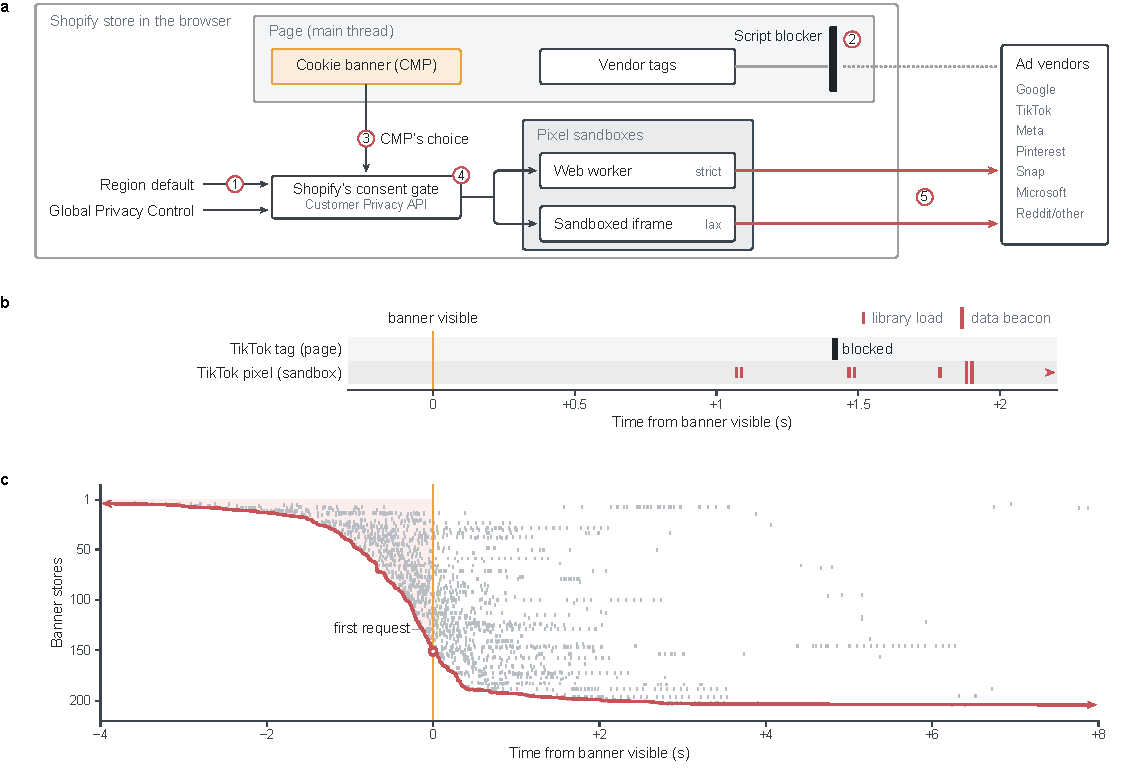
\includegraphics{fig1.pdf}
% GENERATED by paper/integrate_figures_v2.py from figures/v7/fig1/caption_fig1.tex (v2 figure caption, rendered by the figure script).
% Do not edit: change the figure script and re-run build.sh.
\caption{\textbf{Consent is lost at five points between the cookie banner and Shopify's sandboxed pixels.}
(a)~A Shopify store in the browser (outer frame), drawn as nested regions. Top: the page's main thread (light grey ground), where a consent-management platform's (CMP) cookie banner (amber, the colour of its appearance in b and c) and its script blocker (black wall) run; the blocker stops vendor tags in the page (grey line; dotted: the path it cuts). Bottom: Shopify's Web Pixels Manager starts each app or custom pixel in a sandbox isolated from the page (pixel sandboxes, darker grey ground), a web worker (strict runtime) or a sandboxed iframe (lax runtime), once Shopify's consent gate (its Customer Privacy API) allows every purpose that the pixel declares. The gate is set by the store's region default, by the CMP's choice if the CMP writes it to Shopify, and by Global Privacy Control (GPC). The sandboxes stand under the page's vendor tags (the same vendors' code, isolated), and the pixels' requests (brick arrows) leave the browser for the ad vendors underneath the blocker, which covers the page only; the ad-vendor box lists the vendor groups used in every figure. Consent is lost at five of the drawn elements, marked in a by outlined numerals: (1)~the region default, `allowed until choice' on 1,103 of 1,349 stores that returned one (Methods; Fig.~3 measures its effect); (2)~the script blocker (blocked on paper): it cannot see into the sandboxes, so on 46 of 89 stores (51.7\%; Wilson 95\% confidence interval (CI) 41.5--61.8\%) whose CMP listed an ad vendor as blocked and wrote no `yes' to Shopify, that vendor fired from the sandbox anyway in the Default load (no click; main and lower-ranked expansion samples combined; Fig.~4); (3)~the CMP's choice, which arrives late: in loads where a CMP wrote `marketing: no' without a click, 525 of 535 third-party sandboxes that declare marketing had already started (Fig.~5c); (4)~the consent gate, which reads declared purposes only: under GPC, a pixel that declares no purpose fired on 191 of 1,354 stores where Shopify set `sale of data: no' (Fig.~S8c; Fig.~5b counts each store in one class only); (5)~the path to the vendors, which a refusal does not cut: after a Decline (a click on the banner's reject button), a pixel that declares the refused purpose kept sending (same page or unload beacons) on 32 of 196 stores with a recorded refusal (Fig.~5b).
(b)~Point (2) in one page load (re-check, no click). The store is from the main sample; its CMP (Pandectes) lists TikTok as blocked and wrote no `yes'. It is the first by ID among the 5 stores where the blocker neutralized a declared-blocked vendor's page tag while that vendor's sandboxed pixel sent requests, and of its two such vendors TikTok sent more sandboxed requests. The axis is time from the banner becoming visible (amber line), which happened 1.3~s after navigation start; the times below are from navigation start, and no choice was made. The two rows repeat a's grounds (light grey: the page; darker grey: the sandbox). Top row: the blocker neutralized TikTok's tag as it was inserted, at 2.7~s (black bar, the wall of a; script type `javascript/blocked'); the tag sent no request. Bottom row: TikTok's pixel in a sandboxed iframe, which had requested its library 0.34~s earlier, sent 5 library loads (short brick ticks; key above the axis) and 2 data beacons (tall brick ticks) between 2.4 and 3.2~s, and 1 more beacon at 13.2~s (arrowhead at the right end of the row); requests of one kind less than 50~ms apart are drawn side by side. This axis has a larger scale than that of (c); the two zeros are aligned.
(c)~The same failure at scale: every banner store whose sandboxed pixel sent an ad request before any choice (205 of 409 stores that showed a banner), one row each, sorted by its first sandboxed ad request (brick line) and timed from the banner becoming visible (amber line; the detector polls every 250~ms). Grey ticks: the stores' sandboxed ad requests in the Default load; the 55 requests earlier than the axis and the 68 later are not drawn, and the brick line leaves the axis (arrowheads) for the 4 stores whose first request came earlier and the 1 whose first request came later. Rows above the point where the brick line crosses the amber line (open circle; the pale brick ground between the two lines is the time before the banner): the 151 of 205 stores (73.7\%; Wilson 95\% CI 67.2--79.2\%) whose first request came before the banner (Fig.~S6b). Per vendor group: Fig.~S6a; per-store request counts: Fig.~S6e.
All loads from one residential vantage point in California, USA; main sample: 1,358 popular Shopify stores from the Tranco top 200,000.
Panel~(a): Drawn by figure-generation scripts written with AI assistance (Section~\ref{sec:method-ai}).}
\label{fig:situating}

\end{widefig}

Consent measurement has examined banners and what they record: their dark patterns \citep{nouwens2020dark,berens2024cookie} and, in declared-versus-observed audits, consent strings \citep{matte2020banners}, cookie declarations \citep{bollinger2022automating} and consent data \citep{zhang2024cschecker} against observed behaviour. Tracking before a choice or after a rejection is common \citep{papadogiannakis2021post,martinez2022compliance,bouhoula2024automated,martinez2025million}, and rejection and the Global Privacy Control (GPC) signal each remove only part of the tracking cookies \citep{rasaii2025intractable}. US studies have read GPC compliance from privacy strings \citep{zimmeck2023gpc,hausladen2025gpc} and followed opt-outs into advertising systems \citep{liu2024opted,aziz2024johnny}; root-cause studies locate CMP failures in configuration and scanning \citep{tang2025navigating,toth2022dark}. Most such studies audit consent at the banner, in cookies or in consent strings, treating the CMP as the enforcement point.

Where third-party code runs has been studied separately: sandboxes were built to protect a host page from embedded code \citep{terlouw2010adjail,ingram2012treehouse}, trackers slip past users' blockers \citep{bashir2018websockets,dimova2021cname,chen2021filterlist,bottger2026fpt}, and tags under Google Tag Manager's consent layer can leak data \citep{mertens2025gtm}. For Shopify, the one academic consent study we found assessed its native banner \citep{nouwens2025crosscountry}, while the platform, CMP vendors and practitioners document the sandbox, its permissive regional default, blockers that cannot reach app pixels, and pixels that fire before the consent state is set \citep{shopify_aboutpixels,shopify_customerprivacy,truevault_apppixel,onetrust_ecommerce,pandectes_blocking,analyticsninja2025pixels,weltpixel2026race}. Consent audits show what was decided or collected, not which component let the code run; to our knowledge, none fully attributes vendor requests to their execution context and joins them to the platform gate that started their code (Section~\ref{sec:related}). The mechanism is documented, so we claim not its discovery but, to our knowledge, the first measurement of its consequences across stores.

We treat consent as an access-control policy with two enforcement points (Section~\ref{sec:bg-threat}), the CMP's blocker for tags in the main document and Shopify's gate for sandboxed pixels, and lost consent as a request that passes both against the stated policy, a failure of complete mediation \citep{saltzer1975protection}. Our crawler attaches to the page and every worker and iframe, attributes each ad request to its execution context, and joins sandboxed requests to the pixel's declared purposes, Shopify's consent state and the sandbox's start (Fig.~\ref{fig:methods}); comparing these requests with CMP blocklists extends declared-versus-observed auditing \citep{matte2020banners,bollinger2022automating} to execution contexts. This separates a blind blocker from an open or late gate and from a pixel that declared nothing, which cookie-based audits and unattributed network crawls cannot (Section~\ref{sec:disc-beyond}). We load each store with no click (\emph{Default}), a reject click (\emph{Decline}) and GPC, and ask four research questions:
\begin{itemize}
  \item[\RQ{1}] \emph{Before any choice.} On banner stores, how often do sandboxed ad pixels fire before a choice, and with what is this associated?
  \item[\RQ{2}] \emph{Blocked on paper.} When a blocklist, a message to Shopify or the region setting says ``no'' before any choice, how often does a sandboxed pixel fire anyway?
  \item[\RQ{3}] \emph{Choices.} Do Decline and GPC stop sandboxed pixels, and through which path?
  \item[\RQ{4}] \emph{Reach.} What reaches vendors through the requests not stopped?
\end{itemize}
As validation, we test stability and agreement with native GPC.

We loaded 1,358 Shopify storefronts from the Tranco top 200,000 \citep{lepochat2019tranco,tranco_L5PZ4} and 34 creator-linked stores from one residential connection in California; a second crawl added 116 stores from Tranco ranks 200,001--1,000,000 chosen for their CMP blocklists, and piloted Wix, BigCommerce and first-party tag gateways. We find four things. First, before any choice, sandboxed ad pixels fired on 70.2\% of banner stores whose region default allowed tracking and on 24.0\% where it denied it, a gap that held within consent products (Fig.~\ref{fig:region-default}). Second, on 46 of 89 blocklist stores whose CMP had not itself consented, a vendor the blocklist declared blocked fired from the sandbox before any choice, and blocklist stores fired more often than comparable stores, not less (Fig.~\ref{fig:blocked-on-paper}). Third, Shopify's gate held back 2,206 of 2,234 marketing pixels under a denying default, but consent was lost around it: automatic ``no'' writes came after 525 of 535 third-party marketing sandboxes had started, a new sandbox still sent ad requests after a working Decline on 22.9\% of stores, and 34.7\% of stores with sandboxed requests kept sending them under GPC (Fig.~\ref{fig:choices}). Fourth, 63.4\% of sandboxed ad beacons in the Default load carried the full landing URL, query string included (Fig.~\ref{fig:reach}). We also contribute a reusable gate audit, a taxonomy of 24 consent products' Shopify integrations (Table~\ref{tab:cmp-modes}), the pilot (Section~\ref{sec:res-beyond}), fixes, and ConsentCheck, a merchant self-test (Section~\ref{sec:discussion}).

% ============================================================================
\section{Background}\label{sec:background}
% ============================================================================

\subsection{Two consent regimes}\label{sec:bg-law}

In the European Union, prior consent is required before information is stored on or read from a user's device unless it is strictly necessary \citep{eprivacy2002,gdpr2016}, which covers tracking pixels \citep{edpb2023guidelines}; pre-choice tracking there is the standard example of non-compliance \citep{papadogiannakis2021post,bouhoula2024automated}. California follows an opt-out model: under the California Consumer Privacy Act as amended by the California Privacy Rights Act (CCPA), a business may ``sell'' or ``share'' personal information, including for cross-context behavioural advertising, unless the consumer opts out \citep{ccpa2018}. An opt-out preference signal such as GPC must be treated as a valid opt-out \citep{ccparegs7025,caag2022sephora}, and browsers must offer one from 1 January 2027 \citep{ab566}. A pixel that fires before any choice is therefore not by itself prohibited by the CCPA's opt-out rules, but opt-outs must work. Notice at collection, the opt-in rule for consumers under 16 and wiretap law are outside our scope (Section~\ref{sec:disc-law}); we draw no legal conclusions about any store, consent tool or platform.

\subsection{Consent-management platforms and script blocking}\label{sec:bg-cmp}

A CMP displays the banner, records the visitor's choice and, in most products, enforces it with a \emph{script blocker}: code that runs early in the main document and neutralizes tags (new \code{<script>}, \code{<iframe>} and \code{<img>} elements) that match a blocklist of URL patterns grouped into categories such as ``marketing''. A vendor is \emph{declared blocked} on a store when the CMP's machine-readable blocklist lists that vendor's URLs in a category that is blocked before any choice. The blocker cannot see requests made from a web worker, whose network calls never touch the DOM, or the contents of a sandboxed iframe, a separate document with its own origin \citep{whatwg_html}. On Shopify, many CMPs can also report the choice through the Customer Privacy API (\code{setTrackingConsent}); Table~\ref{tab:cmp-modes} lists the integration modes of 24 consent products.

\begin{table}[!tbp]
\centering
\caption{How consent tools can enforce a choice on Shopify. Modes were assigned from each product's downloaded code or its documentation. A mode is a capability, not what a given store has enabled, so the crawler also tested per store whether a Decline click reached Shopify. \emph{Main-thread blocker}: rewrites or holds back tags in the top document. \emph{Writes to Shopify}: calls the Customer Privacy API.}
\label{tab:cmp-modes}
\small
\begin{tabularx}{\linewidth}{@{}l>{\raggedright\arraybackslash}X@{}}
\toprule
Mode & Consent tools (products) \\
\midrule
N: Shopify's own banner & Shopify's native privacy banner (writes to Shopify; no blocker) \\
A: writes to Shopify only & Consentmo, CookieFirst, Fides (Ethyca), Didomi (beta integration), iubenda (with autoblocking off), Enzuzo (vendor claim) \\
B: main-thread blocker only & Usercentrics (without its sync snippet), Transcend (without sync), consentmanager.net; OneTrust and Cookiebot when installed without their Shopify apps \\
C: both & Pandectes, OneTrust (Shopify app), Cookiebot (Shopify app), Osano, CookieHub, Ketch, Clarip, TrustArc (Shopify app) \\
X: unknown & Termly, CookieYes, Cookie-Script, Axeptio, Consentik, Securiti \\
\bottomrule
\end{tabularx}
\end{table}

\subsection{Shopify's Web Pixels Manager and Customer Privacy API}\label{sec:bg-shopify}

On a Shopify storefront, tracking arrives as \emph{app pixels} from Shopify's app store or as \emph{custom pixels} that merchants paste into the admin. An inline loader passes Shopify's Web Pixels Manager (WPM) one configuration entry per pixel: its type, its \code{runtimeContext}, and the privacy purposes it declares (\code{ANALYTICS}, \code{MARKETING}, \code{PREFERENCES}, \code{SALE\_OF\_DATA}) \citep{shopify_aboutpixels,shopify_pixelprivacy}. The WPM starts each pixel in one of three containers (Supplementary Fig.~\ref*{S:fig:s1}): \textbf{STRICT}, a dedicated web worker in which many globals are undefined \citep{shopify_aboutpixels}; \textbf{LAX}, by Shopify's code a hidden sandboxed iframe with an opaque origin, where custom pixels run; and \textbf{OPEN}, a main-thread script that injects the vendor's script, which a CMP blocker can see. In our sample (Table~\ref{tab:pixels}), third-party app pixels appeared on 1,329 stores and were sandboxed in 82\% of cases; TikTok, Pinterest and Snap always ran in STRICT workers and declared sale of data, whereas the Google \& YouTube app ran in OPEN mode and declared no purpose to Shopify.

\begin{table}[!tbp]
\centering
\caption{Web pixels declared by the 1,358 captured main-sample stores (inline WPM configuration of the first usable load; 1,349 stores had one). Stores: stores with the app. Container: the WPM runtime for that app's pixels. The last three columns give the percentage of pixels declaring \code{MARKETING} (Mkt.), declaring \code{SALE\_OF\_DATA} (Sale), or declaring no purpose (None). Pixels declaring no purpose start regardless of the visitor's choice, and only pixels declaring sale of data are stopped by GPC. Shopify's own app and custom pixel entries, present on all 1,349 stores and declaring analytics and marketing, are excluded from the last two rows, which give the number of pixels in parentheses.}
\label{tab:pixels}
\small
\begin{tabularx}{\linewidth}{@{}>{\raggedright\arraybackslash}Xrlrrr@{}}
\toprule
 & & & \multicolumn{3}{c}{\% of pixels declaring} \\
\cmidrule(l){4-6}
App or pixel group & Stores & Container & Mkt. & Sale & None \\
\midrule
\tabinput{tables/pixel_config_table.tex}
\bottomrule
\end{tabularx}
\end{table}

\emph{The gate.} Before creating a pixel's container, the WPM waits until Shopify's consent state allows every purpose the pixel declares; a pixel that declares no purpose starts at once, and if no state can be read every purpose counts as allowed. Pixel callbacks run until the user opts out \citep{shopify_aboutpixels}, and we found no code path that terminates the worker or iframe of a pixel that has already started (Supplementary Fig.~\ref*{S:fig:s1}). Every event the pixels receive carries the page's full URL, including its query string \citep{shopify_aboutpixels}.

\emph{The consent state.} Shopify computes a consent string for each page response from the merchant's region settings and the visitor's location and delivers it in a \code{Server-Timing: \_cmp} header (for example \code{3.AMPS\_USCA\ldots}, where upper-case letters mean that analytics, marketing, preferences and sale of data are allowed for a California visitor); a CMP can overwrite it through \code{setTrackingConsent}. For regions without a consent requirement the default allows all purposes \citep{shopify_customerprivacy}, Shopify's own banner is on by default only for the United Kingdom and the European Economic Area \citep{shopify_privacysettings}, and third-party banners must report consent through the API \citep{shopify_apppixels_help}.

\subsection{Global Privacy Control}\label{sec:bg-gpc}

GPC is a browser signal that asks sites not to sell or share the user's data, sent as a \code{Sec-GPC:~1} request header and exposed as \code{navigator.globalPrivacyControl} in windows and workers \citep{w3c_gpc}; Brave sends it by default, Firefox offers it as a setting, and Chrome and Safari do not send it natively \citep{gpc_site}. Shopify documents that it honours GPC in regions configured for sale-of-data opt-out \citep{shopify_customerprivacy}; in our data it did so regardless of the consent string's region field (Supplementary \ref*{S:sec:s-decline}). It applies GPC on the server when the navigation carries the header and in a main-thread script when the flag is true; either way, GPC gates only pixels that declare \code{SALE\_OF\_DATA}.

\subsection{Threat model: consent as an access-control policy}\label{sec:bg-threat}

We frame the problem as a policy-enforcement failure rather than an attack. The \emph{asset} is the visitor's browsing context: the page URL, which may carry codes that identify a creator or a video, and the identifiers that vendors read. The \emph{policy} combines the merchant's CMP configuration and the visitor's choice, and there are two \emph{enforcement points}: the CMP's main-thread script blocker and Shopify's WPM gate. We infer no intent for the measured stores, which may simply be misconfigured. The design, however, trusts the party it restrains: the gate enforces the purposes that the app developer declares, and a developer who sets them all to false makes the pixel run ``without requiring consent'' \citep{shopify_buildwebpixels}; for a custom pixel, the merchant decides whether permission is required \citep{shopify_custompixels}. A pixel that declares no purpose thus passes both enforcement points without breaking any platform rule. A consent setup can fail in four ways:
\begin{description}
  \item[F1, permissive default.] Before any choice, Shopify's state allows tracking, so the gate opens whatever the banner shows.
  \item[F2, blocked on paper.] A vendor is declared blocked in the CMP's blocklist, but its pixel runs in a sandbox that the blocker cannot reach and still sends requests. We also report the broader case in which the setup says ``no'' through a message to Shopify or the region default.
  \item[F3, lost, late or incomplete choice.] The visitor refuses, but the refusal never reaches Shopify, arrives after the pixels have started, does not stop pixels already running, or is incomplete: it refuses marketing but leaves allowed the sale of data that a pixel declares.
  \item[F4, under-declaration.] A pixel declares no purpose, or fewer than its data flow serves, so a correctly recorded refusal does not gate it; a strategic developer could exploit this. Under GPC, whether pixels that declare marketing but not sale of data under-declare depends on whether their flows are a ``sale'' or ``sharing''.
\end{description}
Figure~\ref{fig:situating}a draws these paths.

% ============================================================================
\section{Related work}\label{sec:related}
% ============================================================================

Table~\ref{tab:positioning} positions this work against its closest neighbours.

\begin{table*}[!tbp]
\centering
\caption{Positioning against the closest related work. Columns: the work studies one hosting platform; attributes requests to the context in which their code runs (worker, iframe, main thread); compares a declared policy or consent state with observed behaviour; audits the enforcement point that starts third-party code (joins the platform's consent state to what starts); has a US vantage point or a GPC arm; checks an emulated GPC signal against a browser's native one. \checkmark: central to the work; (\checkmark): partly, or for another platform or signal; --: not addressed. Marks summarise each paper's main focus as we read it.}
\label{tab:positioning}
\footnotesize\setlength{\tabcolsep}{2.5pt}
\begin{tabularx}{\linewidth}{@{}>{\raggedright\arraybackslash}Xcccccc@{}}
\toprule
Work & Platform- & Context & Declared vs & Enforcement point & US or & Native \\
 & specific & attribution & observed & that starts code & GPC arm & GPC check \\
\midrule
\citealt{matte2020banners} & -- & -- & \checkmark & -- & -- & -- \\
\citealt{bollinger2022automating} & -- & -- & \checkmark & -- & -- & -- \\
\citealt{bouhoula2024automated} & -- & -- & \checkmark & -- & -- & -- \\
\citealt{tang2025navigating} & -- & -- & (\checkmark) & -- & (\checkmark) & -- \\
\citealt{kancherla2025revoke} & -- & -- & (\checkmark) & -- & -- & -- \\
\citealt{zimmeck2023gpc} & -- & -- & (\checkmark) & -- & \checkmark & -- \\
\citealt{rasaii2025intractable} & -- & -- & -- & -- & \checkmark & -- \\
\citealt{hausladen2025gpc} & -- & -- & (\checkmark) & -- & \checkmark & (\checkmark) \\
\citealt{nouwens2025crosscountry} & (\checkmark) & -- & -- & -- & -- & -- \\
\citealt{mertens2025gtm} & \checkmark & (\checkmark) & (\checkmark) & (\checkmark) & -- & -- \\
This work & \checkmark & \checkmark & \checkmark & \checkmark & \checkmark & \checkmark \\
\bottomrule
\end{tabularx}
\end{table*}

\subsection*{Consent banners and declared-versus-observed audits}
Much work measures cookie banners, from the spread of banners and CMPs \citep{degeling2019value,hils2020emergence,kretschmer2021cookie,trevisan2019cookie,sanchezrola2019optout,woods2022commodification} to their dark patterns \citep{nouwens2020dark,berens2024cookie}, and several studies compare what a site or its CMP declares with what the browser observes. \citet{matte2020banners} found TCF consent strings that recorded consent before any choice or after an opt-out; \citet{bollinger2022automating} compared the cookie declarations of four CMP products with the cookies sites actually set; \citet{zhang2024cschecker} compared consent data with behaviour under the GDPR and the CCPA; and \citet{bouhoula2024automated} estimated that 65.4\% of sites that offer a reject option are likely to collect data after rejection. Tracking before a choice or after a rejection is common \citep{papadogiannakis2021post,martinez2022compliance}; GPC and rejection each remove only part of the cookies set \citep{rasaii2025intractable}; sites often fail to inform third parties when consent is revoked \citep{kancherla2025revoke}; and opt-out interfaces often fail to stop third-party tracking \citep{singh2026umbra}. Pre-choice tracking is well established, and we do not claim it as new; what is new in our blocked-on-paper comparison is the attribution of requests to the context in which their code runs, not the comparison itself.

\subsection*{Why CMPs fail}
\citet{tang2025navigating} measured 1,793 sites in eight regions and named, among the root causes of violations, incorrect script embedding (a CMP blocks only tags it recognizes) and incomplete automatic scanning, noting that content loaded only in particular contexts can escape a CMP's scanner. \citet{toth2022dark} showed how CMP configuration flows steer publishers toward non-compliant defaults, \citet{santos2021cmp} discussed the legal role of CMPs, and \citet{dimova2026history} traced banner compliance over time. These works locate the causes in configuration and scanning; we measure an execution-context cause, which no CMP configuration can fix. The only academic measurement of Shopify's consent layer that we found assessed the design of its native banner across 31 national top lists, not what the pixels behind it do \citep{nouwens2025crosscountry}. Consent vendors and practitioners already describe the mechanism \citep{truevault_apppixel,onetrust_ecommerce,pandectes_blocking,analyticsninja2025pixels,weltpixel2026race} without measuring how often it matters; we quantify it.

\subsection*{US opt-outs and GPC}
GPC compliance has been measured through privacy strings: \citet{zimmeck2023gpc} and \citet{hausladen2025gpc} read the US Privacy and GPP strings, OneTrust's consent cookie and \code{/.well-known/\allowbreak gpc.json} to decide whether a site recorded the opt-out. \citet{liu2024opted} and \citet{aziz2024johnny} followed opt-outs from CMPs into advertising systems, \citet{tran2024ccpa,tran2025darkoptout} studied CCPA opt-out links and dark patterns in them, and \citet{zimmeck2024gapc,zimmeck2026android,zimmeck2026gpceu} extended GPC to interface design, Android and EU law; \citet{hils2021conflicting} examined conflicting preference signals. \citet{dawoud2026privaudit} found limited-to-moderate responsiveness of websites to privacy signals and consent choices, and a grey-literature audit found that 55\% of 7,634 California sites set advertising cookies despite GPC \citep{libert2026webxray}. Prior work thus reads consent states, such as TCF strings \citep{matte2020banners} and GPP strings \citep{hausladen2025gpc}, and follows opt-outs into advertising data flows \citep{liu2024opted,aziz2024johnny}; to our knowledge, none attributes vendor requests to the context in which their code runs, or joins them to the platform's gate that starts that code.

\subsection*{Sandboxes and tools that trackers slip past}
Trackers have moved code or traffic to where user-side blocking tools do not look: WebSockets \citep{bashir2018websockets}, CNAME cloaking \citep{dimova2021cname}, scripts that evade filter lists \citep{chen2021filterlist}, and first-party and server-side tracking \citep{bottger2026fpt,jazlan2026sstguard}; two recent systematizations of web tracking do not discuss web workers or platform pixels \citep{vekaria2025sok,rieder2026sok}. Our case differs: the bypassed control belongs to the site itself, and the site's own platform bypasses it, with no intent to evade. The closest analogue of a platform consent gate is Google Tag Manager with Consent Mode, whose tags can leak data \citep{mertens2025gtm,mertens2026gtm80k}. Pixel studies have examined server-side event APIs \citep{elfraihi2024meta}, the Meta pixel's configuration and click identifiers \citep{kieserman2025tracker,ghani2026pixelconfig,bekos2023hitchhiker} and the TikTok pixel's reading of the full page URL \citep{zagi2025referrer}; e-commerce studies have examined dark patterns, cookie policies and data leakage \citep{mathur2019dark,singh2025crumbled,vlachogiannakis2025bought}, and site operators adopt third-party services mainly for convenience \citep{utz2023privacy}. Isolating third-party JavaScript in iframes or web workers was proposed to protect the host page \citep{terlouw2010adjail,ingram2012treehouse}; workers can create privacy risks of their own \citep{karami2021sleeper}, performance libraries move chosen tags into workers \citep{partytown}, and crawler instrumentation can fail to reach some frames \citep{krumnow2022openwpm}, which is why we checked it in every worker and frame. We found no academic study that measures how this isolation interacts with the page's own privacy tool.

% ============================================================================
\section{Methodology}\label{sec:method}
% ============================================================================

Figure~\ref{fig:methods} summarizes the pipeline, which follows earlier large-scale tracking crawls \citep{englehardt2016online}. Every detection and classification step is a deterministic rule (URL patterns, DOM selectors, header decoding, configuration parsing), with no machine learning; Supplementary \ref*{S:sec:s-sample} gives the details.

\begin{widefig}
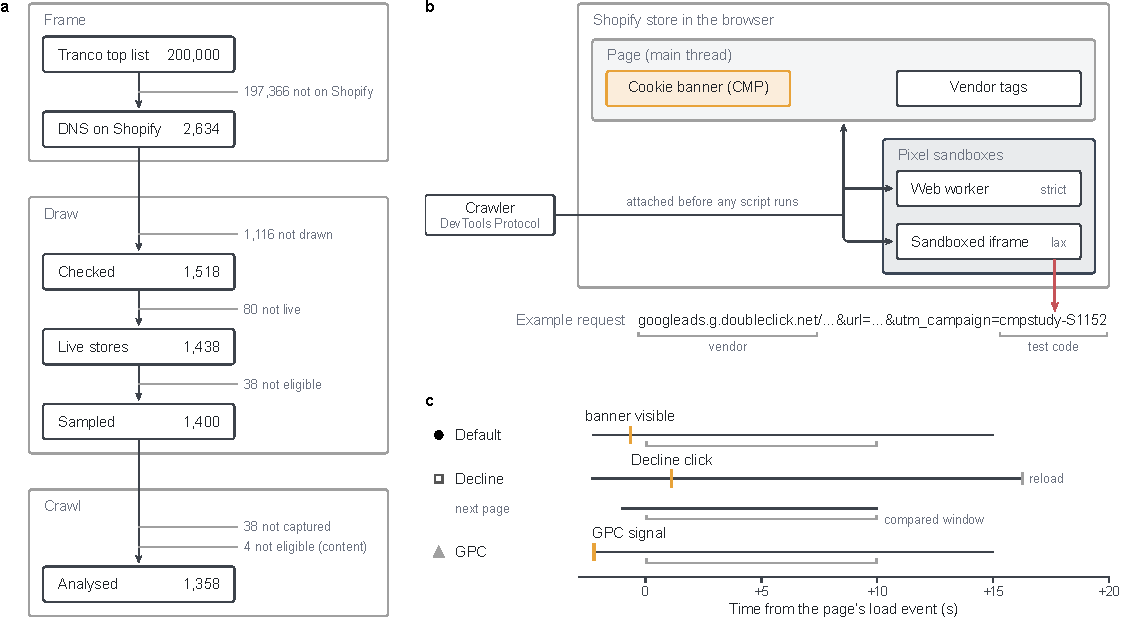
\includegraphics{fig2.pdf}
% GENERATED by paper/integrate_figures_v2.py from figures/v7/fig2/caption_fig2.tex (v2 figure caption, rendered by the figure script).
% Do not edit: change the figure script and re-run build.sh.
\caption{\textbf{We load each store three ways and label every ad request, including those sent from inside Shopify's sandboxes.} (a)~The sampling flow, top to bottom, in three phases, each in a grey outline: Frame (the sampling frame), Draw and Crawl. Each box gives a stage (left) and its count (right); grey branches with flat ends give the domains or stores removed between two stages, with their count and reason, so that each count is the one above minus its branches. Tranco top 200,000 domains; 2,634 whose domain-name system (DNS) records point to Shopify (197,366 not on Shopify by this rule); 1,518 checked: all 902 flagged domains of the three upper rank buckets and 616 of the 1,732 in the lowest, drawn in a seeded random order until its quota of eligible stores was met (the other 1,116 were not drawn); 1,438 live storefronts (80 not live); 1,400 sampled (38 not eligible: no product page, a duplicate, adult or aimed at children; Supplementary Table~\ref*{S:tab:s-exclusions}); 1,358 captured in all three base arms and analysed (38 not captured; 4 not eligible on content: adult products or aimed at children, found after the crawl and excluded for content sensitivity). Not shown: the 34 creator-linked stores of Fig.~6, a separate stratum, not counted in the 1,358. (b)~Where the crawler attaches, drawn on the store of Fig.~1a in its arrangement: a Shopify store in the browser (outer frame), with the page's main thread (light grey ground), which holds the consent-management platform's (CMP) cookie banner (amber) and the vendor tags, and, below it, the two sandboxes in which Shopify's Web Pixels Manager runs pixels (darker grey ground): a web worker (`strict' runtime) above a sandboxed iframe (`lax'). The crawler, a client of the Chrome DevTools Protocol, stands outside the browser; one bus (grey arrows) forks to every target, the page and each worker and iframe, and attaches the crawler to it before any script runs, including the sandboxes, which a CMP's script blocker in the page cannot reach (Fig.~1a). It records each request in the session of the target that sent it and labels every ad request by origin, timing, vendor and payload. Brick arrow: one captured request, the first sandboxed data beacon with our test code in the Default load of store S1152 (one row of Fig.~1c, sent before any choice; brick, as there). A Google Ads pixel sent it from the sandboxed iframe (its origin) 2,720~ms after navigation start, 53~ms before the banner became visible at 2,773~ms (its timing). The arrow lands on our test code in the request's URL below. Square brackets mark the host, which names the vendor, and the test code, cmpstudy-S1152: our pseudonymous code for the store, the value of utm\_campaign in the landing URL that the `url' parameter (the payload) carried. The request path (with the advertiser's account number), the landing page's path and all other parameter values are dropped (\ldots) so that the store cannot be identified. (c)~The three base arms as timelines under one time axis, the time from each page's load event. Each line is one page load and starts at navigation; the marker at the left is the arm's marker used throughout. Amber ticks: each arm's consent moment, named above it. Default (\mkDefault): no interaction; the banner becomes visible (the detector polls every 250~ms), and the load is observed until 15~s after its load event. Decline (\mkDecline): once the banner is visible, the Decline click on a first-layer reject control, made on 240 stores; it worked on 231 (banner gone 2~s after the click, or a refusal recorded by Shopify). The first page is observed after the click and ends at the reload (grey end tick): the same URL is loaded again in the same browser, with new sandboxes, and this next page (the row below) is observed for 10~s after its load event. Global Privacy Control (GPC, \mkGPC): the signal is set from navigation on, in every frame, worker and request. Square brackets: the equal 10~s windows on which the arms are compared (Fig.~5a), each from a load event (in Decline, the next page's), so that they share one zero. Navigation, the banner, the click, the reload and the next page's navigation vary by store and are drawn at their medians over the analysed stores: in Default, navigation 2.3~s and the banner 0.7~s before the load event (1,348 and 406 loads); in Decline (240 clicked loads), the click 1.1~s and the reload 16.3~s after the load event, and the next page's load event 1.0~s after its navigation; in GPC, navigation 2.2~s before the load event. Each base arm covers 1,358 stores. Signal, action, window and $n$ of every arm: Supplementary Table~\ref*{S:tab:s-arms}.
Panels~(a) to~(c): Drawn by figure-generation scripts written with AI assistance (Section~\ref{sec:method-ai}).}
\label{fig:methods}

\end{widefig}

\subsection{Store sample}\label{sec:method-sample}

We took the top 200,000 domains of Tranco list L5PZ4, created on 25 September 2026 \citep{lepochat2019tranco,tranco_L5PZ4}, and flagged a domain if its apex or \code{www} host had an A record in 23.227.32.0/19, the IPv4 block registered to Shopify, or a CNAME chain ending at \code{*.myshopify.com}; 2,634 domains were flagged (Fig.~\ref{fig:methods}a; Supplementary Table~\ref*{S:tab:s-buckets}). A check after the crawl puts the rule's recall at about 83\% (bucket-wise bounds 48--96\%) but only 23\% in the top bucket, and storefronts on \code{shop.} or \code{store.} subdomains, an estimated 1,828 in the top 200,000, are outside the frame (Supplementary \ref*{S:sec:s-sample}).

We stratified by Tranco rank (1--10k, 10k--50k, 50k--100k, 100k--200k), verified all flagged domains in the three upper buckets and, in the 100k--200k bucket, domains in a seeded random order until a quota of 576 eligible stores was met, with one homepage request per site. A domain was eligible if it served a live Shopify Online Store storefront (the one that runs the WPM) with a product page and was neither adult nor aimed at children (content screen: Supplementary \ref*{S:sec:s-extended}; Section~\ref{sec:ethics}). The sample holds 1,400 stores (Supplementary Table~\ref*{S:tab:s-exclusions}); design weights (1 in the census buckets, 2.81 in the 100k--200k bucket) sum to 2,443.5, an estimate of the eligible storefronts in the frame. After the crawl, we excluded 4 of these stores from all analyses for content sensitivity: two adult-product stores that the sampling screen had missed, a toy retailer and a second store that may be aimed at children (Section~\ref{sec:ethics}). The analysed main sample therefore starts from 1,396 stores. We landed on the store's first product link.

A purposive stratum of 34 Shopify stores that YouTube creators link to with a creator-identifying token in the URL (six tokens name a single video) describes these stores only. \storeC is a mixed-audience retailer that markets to children, teenagers and adults, so it would have met the child-directed exclusion; we kept it because the study began from its public creator links, loaded only public pages, involved no data about children and did not load it again after the main crawl. We make no claim about children's data or about COPPA or the CCPA's rules for minors.

\subsection{Measurement arms and crawler}\label{sec:method-arms}

Each store was loaded under three base arms in a per-store shuffled order (Fig.~\ref{fig:methods}c; Supplementary Table~\ref*{S:tab:s-arms}):
\begin{description}
  \item[Default (\mkDefault).] No clicks: we observed until 15~s after the \code{load} event, with six passive mouse-wheel scrolls, one per second, from 2~s into that window.
  \item[Decline (\mkDecline).] We waited up to 10~s for a visible banner, took a screenshot, and clicked a reject control inside it, matched by text or CMP-specific selectors (never Accept, settings or ``Do not sell''). After 15~s we reloaded the URL in the same browser (the ``next page'') and observed for 10~s after its \code{load} event.
  \item[GPC (\mkGPC).] Every request, including worker requests, carried the \code{Sec-GPC:~1} header, and \code{navigator.globalPrivacyControl} was injected into every frame and worker before their first script (checks in Section~\ref{sec:app-validation}).
\end{description}
A seeded 20\% subsample (287 stores) repeated the Default and GPC arms, and a seeded 100-store subsample was loaded in Brave with native GPC and tracker blocking off. The URL was the landing page plus a canary token in its campaign parameters (\code{utm\_campaign=\allowbreak cmpstudy-<store\_id>}). Every load used a new browser with a new temporary profile: Playwright \citep{playwright} with Chromium's headless shell (version 149, 4,876 loads) or Brave (version 150, 100 loads, also headless), with unmodified user agents and no stealth techniques, so pages could tell that the browser was automated (Section~\ref{sec:app-validation}). The crawl ran on 26 September 2026 between 07:03 and 10:01~UTC, with at most one page load per site every 10~s.

\subsection{Instrumentation and request attribution}\label{sec:method-attr}

A client of the browser's DevTools Protocol \citep{cdp} attached automatically to every target (page, out-of-process iframe, worker) and enabled network capture before the target ran, so every request is logged in the session of the target that issued it. A request is \emph{sandboxed} if it was issued inside a worker whose URL matches the WPM's STRICT bootstrap, by a frame whose URL matches a LAX sandbox, or by a frame nested inside such a frame; sandboxed and OPEN requests are joined to their pixel's configuration entry. A rule-based map assigns each request to the advertising vendor whose endpoint \emph{receives} it (seven vendor groups) and separates library loads from data beacons. Payload flags record whether a request carries our canary, the full landing URL or a creator's token, and whether its URL carries a refusal signal of the vendor's own (Supplementary \ref*{S:sec:s-sample} and~\ref*{S:sec:s-extended}).

\subsection{Consent state, CMPs and declared policies}\label{sec:method-consent}

We decoded the \code{Server-Timing: \_cmp} string of each navigation response into the store's region default for our vantage (``allowed until choice'' when marketing is allowed, ``denied until consent'' otherwise), read Shopify's Customer Privacy API about once a second, and recorded every \code{visitorConsentCollected} event. A Decline click \emph{worked} if the banner was gone 2~s later or Shopify recorded an explicit refusal, which held for 231 of 240 clicks; Shopify \emph{recorded a refusal} if a reading after the click had \code{marketing} or \code{trackingConsent} equal to ``no''. CMPs and visible banners were detected by rules, the banners polled every 250~ms (Supplementary \ref*{S:sec:s-sample}). Each store's integration group follows the CMP that showed the banner (Table~\ref{tab:cmp-modes}): Shopify's own banner (N); a CMP that writes to Shopify (A and C); or a blocker-only, unknown or absent CMP (B and X). For Pandectes, OneTrust and Cookiebot the store-specific blocklist is readable in the page, and we recorded for every ad vendor on it whether it was declared blocked before any choice (Supplementary \ref*{S:sec:s-cmp}).

\subsection{Outcomes}\label{sec:method-outcomes}

The primary outcome is store-level: whether at least one \emph{sandboxed ad request} (a data beacon or a library load from a STRICT worker, a LAX iframe or a frame nested in it, to an advertising vendor) occurred in a given window. Because a pixel might ``seemingly load'' while its data gathering is suppressed \citep{truevault_apppixel}, every headline rate is also reported for data beacons only (Supplementary Fig.~\ref*{S:fig:s5}). Rates \emph{before any choice} use the Default load. \emph{After Decline}, the primary outcome is that a sandbox created on the next page sent an ad request within 10~s of its \code{load} event; Default and GPC are compared over the same 10~s. The \emph{gate audit} compares configured pixels whose declared purpose was denied at the moment with the pixels that started.

\subsection{Validation}\label{sec:method-validation}

We checked repeat-load agreement, the GPC injection in every frame and worker \citep{krumnow2022openwpm}, emulated against native GPC, and 54 seeded Decline loads and all 12 forced clicks from saved screenshots (Fig.~\ref{fig:reach}d; Supplementary Fig.~\ref*{S:fig:s4}). A later re-check crawl loaded 128 of the analysed main-sample stores once more, to audit the banner detector's recall and to log which elements a blocker neutralized on the 21 blocklist stores (Supplementary \ref*{S:sec:s-audit}).

\subsection{Statistical analysis}\label{sec:method-stats}

Store-level proportions carry Wilson 95\% confidence intervals \citep{wilson1927probable}, and headline rates also, as a sensitivity analysis, a BCa cluster bootstrap by consent tool \citep{field2007bootstrapping}, because banner behaviour is a property of the consent product. Paired differences between arms carry Newcombe's interval for paired data \citep{newcombe1998paired}, other differences his interval for independent samples \citep{newcombe1998independent}, and stratified differences are Mantel--Haenszel estimates \citep{mantel1959statistical}. Intervals for shares whose unit is not a store resample stores (a percentile bootstrap, or the Korn--Graubard interval \citep{korn1998survey}), Cohen's $\kappa$ \citep{cohen1960kappa} is read against \citet{landis1977agreement}, and Firth-penalized logistic models \citep{firth1993bias,heinze2002separation} are exploratory. The primary estimates are the three headline rates (pre-choice firing on banner stores, the fresh-page residual after Decline and the residual under GPC), the blocked-on-paper rate on stores whose CMP had not itself consented (pooled over the main sample and the expansion), and the paired difference between Decline and GPC; other intervals are descriptive and not adjusted for multiplicity (further details: Supplementary \ref*{S:sec:s-extended}). One script regenerates the analysis outputs from the saved crawl data, and an automated check traces every number in the manuscript to those outputs or, for the literature, to the cited papers.

\subsection{Round 4: blocklist expansion and a pilot beyond Shopify}\label{sec:method-r4}

A second crawl on 27 September 2026 ran the same crawler and arms, at most six concurrent browsers and at least 10~s between two loads of a site; unlike the main crawl, it fetched each site's \code{robots.txt} first and loaded a site only if it allowed the page (Section~\ref{sec:ethics}). \emph{Expansion.} Screening Tranco ranks 200,001--1,000,000 with the main sample's DNS and eligibility rules found, among 11,354 eligible storefronts, 120 whose readable Pandectes or OneTrust blocklist declared an ad vendor blocked before any choice for a California visitor or could only be settled at run time; all were loaded, 116 were captured in all three arms, and on 96 the blocklist was in force at run time. The blocked-on-paper estimands were computed by the main pipeline's own code, which reproduced every main-sample value exactly. \emph{Pilot.} We selected 80 Wix and 80 BigCommerce sites, 26 sites that send Google tags through a first-party gateway (a tag endpoint on the site's own domain), and all 8 Partytown sites and 1 Cloudflare Zaraz site that the screen found. First-party requests were attributed to a vendor only when their wire format named it, and server-side forwarding was never inferred (Supplementary \ref*{S:sec:s-r4}).

\subsection{Changes to the planned protocol}\label{sec:method-deviations}

The study had no public preregistration; the planned protocol and eight predictions about the mechanism were written in an internal note before the crawl, and Supplementary Table~\ref*{S:tab:s-predictions} reports how each fared. Three changes were made during the crawl, the largest that most loads ran at ten rather than the planned six concurrent browsers, with per-site pacing unchanged; three checks were added after the analyses (Supplementary \ref*{S:sec:s-extended}).

\subsection{Use of generative AI}\label{sec:method-ai}

During the preparation of this work the author used Anthropic's Claude to assist with writing and debugging the measurement, analysis, and figure-generation scripts. The author reviewed the code and its outputs and takes full responsibility for the content of the publication. The validation labels (the 21 content-screen decisions, the screenshot audits of 54 Decline loads and 12 forced clicks, and the blind recall audit of the 128 re-check loads) were made with the same assistance rather than by an independent human rater, so they are not an independent validation; a kit for blind re-labelling is released with the data.

% ============================================================================
\section{Results}\label{sec:results}
% ============================================================================

Of 4,976 planned loads, 119 (on 38 stores) were unusable (Supplementary Table~\ref*{S:tab:s-failures}); 23 stores looked like bot blocking, which we did not try to get around. After the 4 stores excluded for content sensitivity (Section~\ref{sec:method-sample}), 1,358 of the remaining 1,396 main-sample stores and all 34 creator stores were captured in all three base arms. Table~\ref{tab:headline} collects the headline estimates.

\begin{table}[!tbp]
\centering
\caption{Headline estimates (main sample unless marked; unweighted). CI: Wilson 95\% interval; for rows marked $^\dagger$ the cluster bootstrap by consent tool is given in brackets. ``Sandboxed'': sent from a Shopify STRICT worker, a LAX iframe or a frame nested in one; a request is a data beacon or a library load. Last row: paired difference in percentage points (pp) with Newcombe's interval.}
\label{tab:headline}
\footnotesize\setlength{\tabcolsep}{4pt}
\begin{tabularx}{\linewidth}{@{}>{\raggedright\arraybackslash}Xrrl@{}}
\toprule
Statistic & $k$/$n$ & \% & 95\% CI \\
\midrule
\multicolumn{4}{@{}l}{\emph{Before any choice (Default)}}\\
Consent banner shown & 409/1,358 & 30.1 & 27.7--32.6 \\
Sandboxed ad request, all stores$^\dagger$ & 803/1,358 & 59.1 & 56.5--61.7 [55.7--62.3] \\
Sandboxed ad request, banner stores$^\dagger$ & 205/409 & 50.1 & 45.3--54.9 [32.6--58.9] \\
\quad default ``allowed until choice''$^\dagger$ & 165/235 & 70.2 & 64.1--75.7 [63.0--79.1] \\
\quad default ``denied until consent''$^\dagger$ & 40/167 & 24.0 & 18.1--31.0 [16.5--36.3] \\
\quad \quad pixel not declaring marketing & 32/167 & 19.2 & 13.9--25.8 \\
First sandboxed request $>$1 poll before banner & 108/205 & 52.7 & 45.9--59.4 \\
\midrule
\multicolumn{4}{@{}l}{\emph{Blocked on paper: declared vendor fired from the sandbox}}\\
CMP wrote no ``yes'' (primary), both samples & 46/89 & 51.7 & 41.5--61.8 \\
\quad main sample & 7/14 & 50.0 & 26.8--73.2 \\
\quad expansion, ranks 200k--1M & 39/75 & 52.0 & 40.9--62.9 \\
All blocklist stores, both samples & 67/117 & 57.3 & 48.2--65.9 \\
Configured sandboxed pixel of that vendor & 10/15 & 66.7 & 41.7--84.8 \\
CMP told Shopify ``marketing: no'': sandboxed request & 39/65 & 60.0 & 47.9--71.0 \\
\midrule
\multicolumn{4}{@{}l}{\emph{Decline}}\\
No first-layer reject option (banners found) & 165/405 & 40.7 & 36.1--45.6 \\
Refusal recorded (working clicks) & 196/231 & 84.8 & 79.7--88.9 \\
New sandbox fired on the fresh page (working clicks)$^\dagger$ & 53/231 & 22.9 & 18.0--28.8 [17.4--29.5] \\
Any sandboxed request after the click (working clicks) & 80/231 & 34.6 & 28.8--41.0 \\
\midrule
\multicolumn{4}{@{}l}{\emph{GPC}}\\
``Sale of data: no'' (loads with a readable state) & 1,166/1,169 & 99.7 & 99.2--99.9 \\
At-risk loads in which a sale-of-data pixel started & 0/1,264 & 0.0 & 0.0--0.3 \\
Still sending, of stores sandboxed under Default$^\dagger$ & 279/803 & 34.7 & 31.5--38.1 [30.9--38.7] \\
\midrule
Blocklist minus no declaration, both samples (Mantel--Haenszel), pp & & 13.4 & 4.0 to 22.8 \\
Decline minus GPC (53 vs 41 of 231 stores), pp & & 5.2 & 0.2 to 10.3 \\
\bottomrule
\end{tabularx}
\end{table}

% ----------------------------------------------------------------------------
\subsection{RQ1: Sandboxed pixels fire before any choice}\label{sec:res-prechoice}
% ----------------------------------------------------------------------------

Before any click, an ad request left the page on 1,254 of 1,358 stores (92.3\%, 95\% CI 90.8--93.6\%), and a \emph{sandboxed} one on 803 (59.1\%, 56.5--61.7\%). A consent banner appeared on 409 stores (30.1\%), and on half of these a sandboxed ad pixel fired before any choice: 205 of 409 (50.1\%, 45.3--54.9\%; Fig.~\ref{fig:situating}c; per vendor group: Supplementary Fig.~\ref*{S:fig:s6}a), against 598 of 949 stores without a banner (63.0\%, 59.9--66.0\%; Supplementary Fig.~\ref*{S:fig:s6}e). Neither library loads nor missed banners explain this (Supplementary \ref*{S:sec:s-extended}).

\begin{widefig}
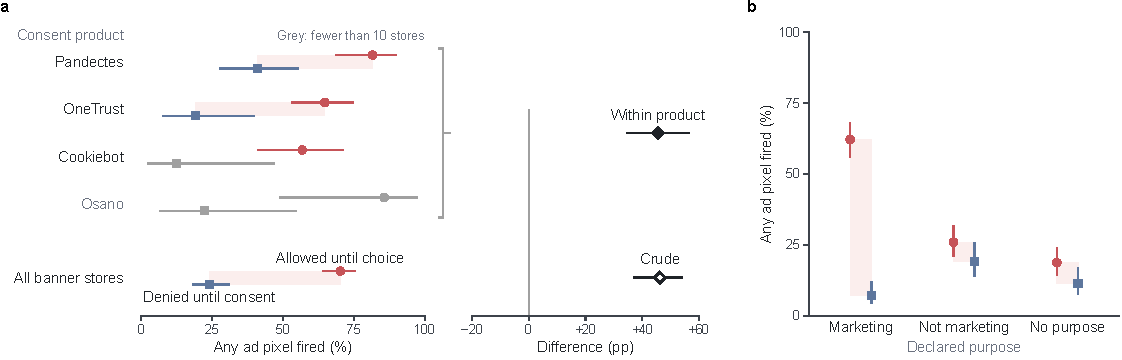
\includegraphics{fig3.pdf}
% GENERATED by paper/integrate_figures_v2.py from figures/v7/fig3/caption_fig3.tex (v2 figure caption, rendered by the figure script).
% Do not edit: change the figure script and re-run build.sh.
\caption{\textbf{Before any choice, whether sandboxed pixels fire tracks Shopify's region default, even within the same consent tool.} (a)~Left: share of banner stores on which an ad pixel running in a Shopify sandbox sent a request before any choice, by Shopify's region default at our California vantage point: `allowed until choice' (brick circles, just above each row's centre line) and `denied until consent' (slate squares, just below it). Rows: the 4 consent-management platform (CMP) products with at least 5 stores under each default, in order of their Mantel--Haenszel (MH) weight; stores that fired / stores, `allowed' then `denied': Pandectes 40/49 and 18/44; OneTrust 44/68 and 4/21; Cookiebot 21/37 and 1/8; Osano 6/7 and 2/9. Bottom row, set apart: all 402 banner stores with a readable default, 165 of 235 (70.2\%; 95\% confidence interval (CI) 64.1--75.7\%) against 40 of 167 (24.0\%; 18.1--31.0\%). A group of fewer than 10 stores is drawn grey, as the note in the plot says (Cookiebot's `denied' group and both of Osano's; a row with no coloured group has its name in grey). Pale brick band: the excess under `allowed until choice', from the `denied' share to the `allowed' share, drawn where both groups are coloured. Right, on the same rows and the same scale: the difference, `allowed' minus `denied', in percentage points (pp), with its 95\% CI (horizontal line), against a grey zero line: pooled within product by the MH method with Sato's variance (filled diamond, `Within product', level with the middle of the product rows, which a grey bracket groups) +45.6~pp (34.6--56.6), and over all banner stores (open diamond, `Crude', on their row; Newcombe's interval) +46.3~pp (36.9--54.3). The pooled difference uses all 12 CMP products with stores under both defaults (354 stores; the other 48 use a product seen under one default only, or none); the 4 drawn on the left carry 84\% of its weight. The other 8, with fewer than 5 stores under one default, are not drawn: Usercentrics 5/6 and 0/3; iubenda 6/8 and 1/2; Ketch 2/2 and 1/5; Clarip 2/4 and 0/2; Shopify's banner 1/1 and 11/65; CookieScript 4/5 and 1/1; CookieYes 4/4 and 0/1; consentmanager 0/1 and 1/1. The 7 banner stores without a readable default are not shown; none of them fired. (b)~The same measure, counting only the pixels that declare a given purpose, with the markers of (a) (brick circles `allowed until choice', slate squares `denied until consent'), its intervals and pale brick bands, and the same scale: `marketing' 146 of 235 (62.1\%) against 12 of 167 (7.2\%); not `marketing' 61 of 235 (26.0\%) against 32 of 167 (19.2\%); no purpose at all (a subset of not `marketing') 44 of 235 (18.7\%) against 19 of 167 (11.4\%). A store can count under more than one purpose. On 11 of the 12 `denied' stores with a firing `marketing' pixel, the CMP had first told Shopify `yes' without a click. Lines through the circles and squares: Wilson 95\% CIs, each in the colour of its mark (stores are the unit). All three plots share one scale (the same length per percentage point). Default load (no interaction); main sample 1,358 stores, 409 with a banner. Per-vendor rates, the timing of the first sandboxed request, request origins and per-product shares: Fig.~S6.}
\label{fig:region-default}

\end{widefig}

Pre-choice firing on banner stores was most strongly associated with Shopify's region default (Fig.~\ref{fig:region-default}a): it occurred on 165 of 235 banner stores (70.2\%, 64.1--75.7\%) where the consent string allowed marketing until the visitor chose, and on 40 of 167 (24.0\%, 18.1--31.0\%) where it denied marketing until consent. This contrast, specified before the crawl (prediction P1), is partly confounded with the consent product but persists within products (Mantel--Haenszel difference over 12 products 45.6 percentage points, 95\% CI 34.6 to 56.6). For pixels that declare marketing, which the gate is meant to hold back, the contrast is sharper, 146 of 235 (62.1\%) against 12 of 167 (7.2\%), and on 11 of those 12 stores the CMP had told Shopify ``yes'' without any click. This is F1: the sandbox follows Shopify's state, and the banner matters only insofar as the CMP changes that state.

The ``denied until consent'' stores are the closest this vantage point comes to an opt-in regime such as the EU's. On 32 of these 167 banner stores (19.2\%, 13.9--25.8\%), a sandboxed ad request before any choice came from a pixel that does not declare marketing, and on 19 (11.4\%, 7.4--17.1\%) from one that declares no purpose at all: an opt-in default does not hold back pixels that do not declare the purpose it withholds (F4).

Because the banner detector polled every 250~ms, a request counts as preceding the banner only if it came more than one polling interval earlier. On 108 of the 205 banner stores with a pre-choice sandboxed request (52.7\%, 45.9--59.4\%), the first request came that early (Supplementary Fig.~\ref*{S:fig:s6}b), and on 151 (73.7\%) before the banner at all; the per-store flag repeated only moderately (Cohen's $\kappa=0.54$ on 46 repeat stores). Where the first request clearly preceded the banner, no choice could have prevented it (Fig.~\ref{fig:situating}c).

The sandbox carried 31.5\% (29.8--33.2\%) of the 40,016 ad requests in Default loads, most for vendors whose app pixels run in STRICT workers (Supplementary Fig.~\ref*{S:fig:s6}c and Table~\ref*{S:tab:s-vendor}).

% ----------------------------------------------------------------------------
\subsection{RQ2: Blocked on paper}\label{sec:res-paper}
% ----------------------------------------------------------------------------

We next asked what happens when a store's consent setup says ``no'' before any choice (Fig.~\ref{fig:blocked-on-paper}; Supplementary Fig.~\ref*{S:fig:s7}). In the main sample, on 21 stores (15 Pandectes, 5 OneTrust and 1 Cookiebot store), a readable blocklist declared at least one ad vendor blocked before any choice. A blocklist is in force only while the CMP has not consented, and on 7 of the 21 the CMP itself wrote ``marketing: yes'' to Shopify without any click, on 2 of them through an optional Pandectes merchant setting that grants consent to automated browsers (Section~\ref{sec:app-validation}). On the other 14 stores the declared-blocked vendor's own pixel sent requests from Shopify's sandbox before any choice on 7 (50.0\%, 26.8--73.2\%).

Fourteen stores give a wide interval, so the expansion crawl (Section~\ref{sec:method-r4}) added 116 stores from ranks 200k--1M, on 96 of which (93 Pandectes, 3 OneTrust) the blocklist was in force at run time. On 21 of the 96 the CMP wrote ``yes'' without a click; on 39 of the other 75 the declared vendor fired from the sandbox (52.0\%, 40.9--62.9\%), a rate no different from the main sample's (difference $-2.0$ percentage points, 95\% CI $-27.6$ to 23.7). Our primary estimate therefore pools the two samples: on 46 of 89 stores (51.7\%, 41.5--61.8\%) a vendor that the blocklist declared blocked sent requests from Shopify's sandbox before any choice, and on 37 (41.6\%, 31.9--52.0\%) it did so from a pixel that declares marketing. Over all 117 blocklist stores the rate was 67 (57.3\%, 48.2--65.9\%); design-weighted and alternative estimates are in Supplementary \ref*{S:sec:s-r4} and~\ref*{S:sec:s-extended}.

\begin{widefig}
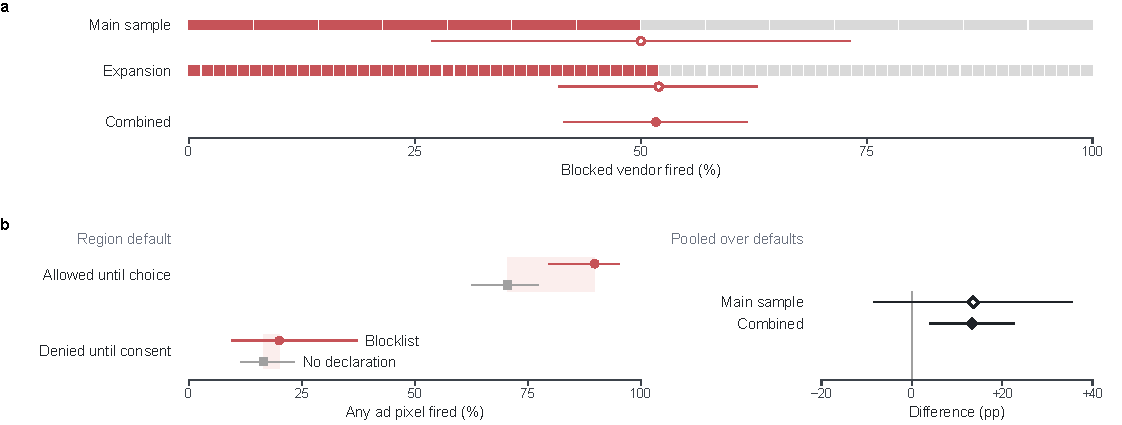
\includegraphics{fig4.pdf}
% GENERATED by paper/integrate_figures_v2.py from figures/v7/fig4/caption_fig4.tex (v2 figure caption, rendered by the figure script).
% Do not edit: change the figure script and re-run build.sh.
\caption{\textbf{Blocked on paper: a vendor that the consent tool's blocklist declares blocked still fired from Shopify's sandbox on about half of the stores, and blocklist stores fired more, not less, often than comparable stores.} (a)~Point~(2) of Fig.~1a at scale: blocklist stores whose consent-management platform (CMP) wrote no `marketing: yes' to Shopify in the Default load (no interaction), and whether the ad vendor that the CMP's blocklist declared blocked sent a request from its sandboxed Shopify pixel before any choice. Each bar is one sample, one cell per store across the full axis: brick cells, the stores on which the declared-blocked vendor fired, drawn first so that the brick part ends at the share; light grey cells, the stores on which it did not. Under each bar, the sample's share (open circle) with its 95\% confidence interval (CI): main sample (Tranco top 200,000) 50.0\% (7 of 14), expansion 52.0\% (39 of 75). Below a gap, the combined sample, the primary estimate (filled circle): 51.7\% (46 of 89; 95\% CI 41.5--61.8\%). The expansion (Round~4) adds the 96 Shopify stores from Tranco ranks 200,001--1,000,000 whose blocklist was in force at run time. (b)~Like for like, among stores whose CMP wrote no `yes': share of stores on which any sandboxed ad pixel sent a request before any choice, within Shopify's region default at our California vantage point (one pair of rows each). Brick circles (upper row): blocklist stores of both samples; grey squares (lower row): the comparison, main-sample banner stores without a readable declaration. `Allowed until choice' 89.8\% (53 of 59) vs 70.5\% (98 of 139); `denied until consent' 20.0\% (6 of 30) vs 16.6\% (24 of 145). Pale brick ground: the gap between a pair's two shares, that is, how much more often the blocklist stores fired. Right, on rows of its own between the two pairs (it belongs to neither default) and at the same scale (one percentage point has the same length in both plots): that gap pooled over the two defaults, blocklist minus no declaration, by the Mantel--Haenszel method with Sato's variance, as a diamond with its 95\% CI against a grey zero line (as in Fig.~3a, right). Combined (filled diamond), blocklist stores fired +13.4 percentage points (pp; 95\% CI 4.0--22.8) more often, so a reduction is ruled out; main sample only (open diamond), +13.6~pp ($-$8.4 to 35.6). Horizontal lines: uncapped 95\% CIs, each in the colour of its mark (Wilson for a share; stores are the unit). Open marks: one sample alone; filled marks: the combined sample. Brick marks the blocklist stores (consent lost) in both panels and pale brick their excess; grey, the comparison stores and context; near-black, the pooled difference. Blocklists are readable for Pandectes, OneTrust and Cookiebot only. Main sample 1,358 stores; Default load unless stated. The blocklist entries by route, from Shopify's sandbox or from a page script: Fig.~S7d.}
\label{fig:blocked-on-paper}

\end{widefig}

A blocklist did not reduce sandboxed firing; blocklist stores fired more often. Comparing any sandboxed ad pixel like for like within Shopify's region default, among stores whose CMP wrote no ``yes'', blocklist stores of both samples fired on 53 of 59 against 98 of 139 main-sample banner stores without a readable declaration where the default allowed marketing, and on 6 of 30 against 24 of 145 where it denied it (Mantel--Haenszel difference 13.4 percentage points, 95\% CI 4.0 to 22.8; Fig.~\ref{fig:blocked-on-paper}b). This falsification test of prediction P1 rules out any reduction; in the main sample alone the difference was 13.6 percentage points (95\% CI $-8.4$ to 35.6), which could not. The reference stores are all from the top 200,000, and the expansion stores are lower-ranked and almost all use Pandectes, so the excess need not be caused by the blocklist; what the comparison excludes is that the blocklist held sandboxed pixels back. Shopify's state decided instead: over all 117 blocklist stores, the declared vendor fired on 51 of the 72 whose default allowed marketing (70.8\%), close to the 70.7\% of undeclared banner stores with that default, and on 16 of the 45 whose default denied it. Two policies governed the same code, and only Shopify's was enforced (F2).

Two observations in the main sample show the mechanism directly. In a later re-check load, the blocker neutralized a declared vendor's main-document tag while that vendor's pixel sent requests from Shopify's sandbox on 5 stores (one of them: Fig.~\ref{fig:situating}b); and on 8 stores (an exploratory analysis) the CMP's own blocklist pattern, such as the URL of TikTok's pixel library, matched a URL that the sandbox fetched, so the blocker would have neutralized the identical request in the main document. Although Pandectes documents that for Shopify-managed apps it signals consent rather than blocks \citep{pandectes_blocking}, a blocklist entry is still a declaration: it is in the merchant's configuration, is enforced for main-thread tags, and is what the merchant sees. The blocker and the write to Shopify are two parts of one design, and the limit lies in Shopify's architecture rather than in any one product: no consent tool on Shopify can block a sandboxed pixel (Table~\ref{tab:cmp-modes}). A message to Shopify helped only if it came first: where the CMP told Shopify ``marketing: no'' before any click (65 stores), a sandboxed ad pixel had already fired on 39 (60.0\%, 47.9--71.0\%; Section~\ref{sec:res-race}).

At the level of entries (primary set: Supplementary Fig.~\ref*{S:fig:s7}d; all stores: \ref*{S:fig:s7}b), 29 of the 104 declared-blocked ad-vendor entries had a configured sandboxed pixel of the same vendor on the store, and 21 of these (72.4\%, 42.5--92.3\%, clustered by store) fired from the sandbox; store--vendor pairs and entries without a configured pixel are reported in Supplementary \ref*{S:sec:s-extended}.

% ----------------------------------------------------------------------------
\subsection{RQ3: Do Decline and GPC stop sandboxed pixels?}\label{sec:res-choices}
% ----------------------------------------------------------------------------

\subsubsection{Decline}\label{sec:res-decline}

Of the 405 banners found in the Decline arm, 165 (40.7\%, 36.1--45.6\%) offered no first-layer reject control, typically US ``notice-only'' banners; on the other 240 stores we clicked it, and 231 clicks worked. Shopify recorded an explicit refusal after 196 of them (84.8\%, 79.7--88.9\%); marketing was still allowed after 20 clicks, and the state was unreadable after 15.

On a fresh page, the reload after the click, a newly created sandbox still sent an ad request on 53 of the 231 stores (22.9\%, 18.0--28.8\%; Fig.~\ref{fig:choices}a), against 45.9\% under Default in the same 10~s window, a paired reduction of 22.9 percentage points (95\% CI 17.4 to 28.3): about half of the Default-positive stores kept firing. Any sandboxed request after the click occurred on 80 stores (34.6\%). By integration group, exploratory models found no clear difference after adjustment (Supplementary Fig.~\ref*{S:fig:s8}b and \ref*{S:sec:s-models}).

\begin{widefig}
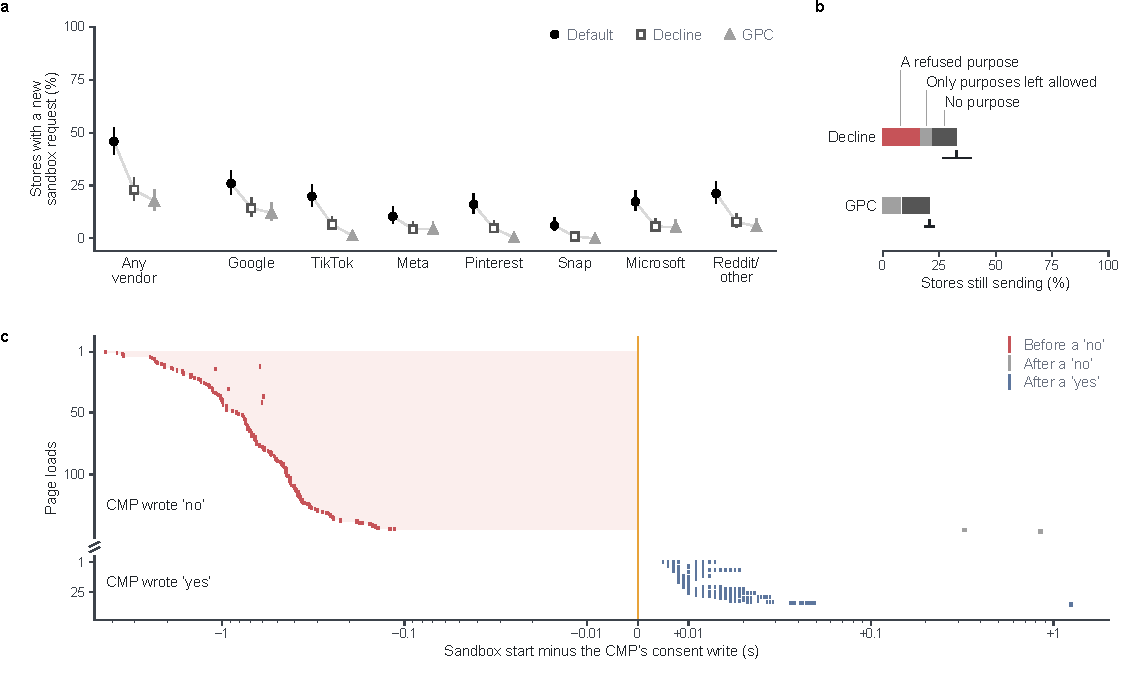
\includegraphics{fig5.pdf}
% GENERATED by paper/integrate_figures_v2.py from figures/v7/fig5/caption_fig5.tex (v2 figure caption, rendered by the figure script).
% Do not edit: change the figure script and re-run build.sh.
\caption{\textbf{A refusal stops new pixels that declare the refused purpose; pixels that started earlier, declare other purposes or declare none keep sending.}
(a)~The 231 stores where the Decline click worked, each loaded three ways: Default, and with a refusal (Decline, or the Global Privacy Control (GPC) signal). Share of stores on which a newly created sandbox (a Shopify web-pixel worker or iframe) sent an advertising request within 10~s, for any vendor and for each of the seven vendor groups. Any vendor: Default 106 of 231 (45.9\%; 95\% confidence interval (CI) 39.6--52.3); the fresh page after Decline 53 of 231 (22.9\%; 18.0--28.8); GPC 41 of 231 (17.7\%; 13.4--23.2). In every group Default is the highest of the three, and no store fired after Decline or under GPC without also firing under Default. Paired differences: Default $-$ Decline 22.9 percentage points (pp; 95\% CI 17.4--28.3); Default $-$ GPC 28.1~pp (22.2--33.9); Decline $-$ GPC 5.2~pp (0.2--10.3; 23 stores fired only after Decline and 11 only under GPC, exact McNemar $p = 0.058$). In each group the three loads of the same stores sit left to right in the arm coding of Fig.~S8a (filled black circle: Default; open dark-grey square: Decline; filled grey triangle: GPC; key at the top right), joined by a thin light-grey line, on the full percentage scale; the vendor groups are named on the x axis, with any vendor set apart on the left (per-vendor values, on the same scale: Fig.~S8a). Vertical lines: Wilson 95\% CIs; paired differences: Newcombe hybrid-score intervals.
(b)~Shopify's gate held the new pixels that declare the refused purpose (not drawn): after Decline, 0 of 196 stores had a new pixel declaring it; under GPC, 0 of 7,458 configured pixel entries that declare ``sale of data'' started (0 of 1,264 at-risk loads; 0 stores); while the region default denied ``marketing'', 2,206 of 2,234 entries that declare it were held (98.7\%; the other 28 started). The bars show what still got through: the share of stores that still sent a sandboxed ad request despite the refusal, Decline 64 of 196 (32.7\%; 95\% CI 26.5--39.5) and GPC 279 of 1,354 (20.6\%; 18.5--22.8). Each such store is in one class, assigned in the order a refused purpose, only purposes left allowed, no purpose; each thin bar stacks the classes from 0 in that order, and the classes are named once, at the Decline bar: a refused purpose (brick: a pixel that started before the refusal and declares the refused purpose kept sending, on the same page or in an unload beacon; Decline only, 32 stores), only purposes left allowed (grey; Decline 11, GPC 111), no purpose (dark grey; Decline 21, GPC 167). The greys of (b) mark these classes, not the arms of (a). Fig.~S8c uses the same class names, colours and order, by window and without the one-class-per-store rule. The GPC total includes 1 store that matched no class (not drawn). Decline: the 196 stores where Shopify recorded the refusal; GPC: the 1,354 stores where Shopify set ``sale of data: no''. Just under each bar: its total (a short tick rising toward the bar's end) on its Wilson 95\% CI (horizontal line).
(c)~The race between a consent-management platform (CMP) and pixel start-up: one row per page load in which a CMP wrote ``marketing: no'' to Shopify without a click (146 loads, 99 stores; upper block) or ``yes'' (35 loads, 23 stores; lower block); the row ticks count the loads within each block, so the row axis is broken between the blocks (cut marks). Each tick is one third-party sandbox that declares ``marketing'', at its start minus the CMP's consent write (amber line); rows are sorted by the load's first sandbox. The time axis is logarithmic on both sides of the write and linear between the two ticks nearest it, so that starts seconds before the write and milliseconds after it are both visible; every sandbox is drawn. The pale brick ground runs, row by row, from a ``no'' load's first sandbox to the write: the time its marketing sandboxes ran before the refusal arrived. Of the 535 sandboxes in the ``no'' loads, 525 started before the write (brick; median 653~ms before) and 10 after it (grey); all 342 in the ``yes'' loads started after it (slate; median 14~ms after); the key at the top right names the three tick colours. Throughout, brick marks consent lost (b, c), slate consent honoured (c), amber the consent moment (c) and grey context.}
\label{fig:choices}

\end{widefig}

Why does firing continue after a refusal that Shopify recorded? Figure~\ref{fig:choices}b classes each store once, and Supplementary Fig.~\ref*{S:fig:s8}c classes each residual sandboxed request by what its pixel declares and by Shopify's state at the time. New sandboxes of pixels declaring a refused purpose fired on none of the 196 stores: the gate held. Pixels started before the click that declare a refused purpose kept sending on 32 stores (16.3\%, 11.8--22.1\%), on the same page (19) or as unload beacons when the page reloaded (20), which any navigation away triggers (F3); their initiator stacks cannot separate events that Shopify delivered after the opt-out from the vendor's own timers. On 13 stores (6.6\%, 3.9--11.0\%) the pixel declared only purposes that the Decline had left allowed: CMPs recorded the Decline as a refusal of marketing, and sale of data stayed allowed on 112 of the 196 stores (F3, an incomplete refusal). On 28 stores (14.3\%, 10.1--19.9\%) the pixel declared no purpose (F4). Merchants' custom pixels were involved on 34 of the 37 stores with a fresh-page residual (Supplementary \ref*{S:sec:s-decline}).

\subsubsection{GPC}\label{sec:res-gpc}

Shopify honoured GPC: \code{saleOfDataAllowed()} was false in 1,166 of the 1,169 GPC loads with a readable state, and no configured pixel entry declaring sale of data started (0 of 7,458 entries in 1,264 loads at risk; upper 95\% bound 0.3\% of loads) or sent a request on any of the 1,354 stores where Shopify showed ``sale of data: no'' (Fig.~\ref{fig:choices}b). Yet of the 803 stores with a sandboxed ad request under Default, 279 (34.7\%, 31.5--38.1\%) still sent one under GPC: on 111 of the 1,354 stores from pixels declaring only purposes that GPC leaves allowed, mostly marketing (100), which Shopify's mapping of GPC to sale of data does not cover, and on 191 from pixels declaring no purpose (F4). Custom pixels alone accounted for the residual on 182 of the 279 stores.

Compared for persistence after the choice (the same 231 stores, new sandboxes on a later page, 10~s windows), a sandboxed ad request occurred on 53 stores after Decline and 41 under GPC (22.9\% and 17.7\%), a paired difference of 5.2 percentage points (95\% CI 0.2 to 10.3; exact McNemar $p=0.058$): GPC's advantage was between about 0 and 10 points. Over the whole visit the controls differ much more, because a Decline user is exposed before the click: a sandboxed ad request came before the click on 101 of these stores, against 41 over the whole GPC load (difference 26.0 percentage points, 95\% CI 20.0 to 31.7), although the pre-click window is the shorter. Counting attempted rather than working Declines changes little (Supplementary \ref*{S:sec:s-extended}).

\subsubsection{The gate held; the race was often lost}\label{sec:res-race}

To separate the gate from its inputs, we compared configured pixels at risk with the pixels that started. Beyond GPC (above), under a denying region default 2,206 of 2,234 marketing-declaring entries (98.7\%, 94.4--99.9\%, clustered by store) were held back in loads without a CMP ``yes''. Of 6,983 starts under a partly denied state by pixels that declare a purpose, 97 had a declared purpose denied at that moment; they came from 10 loads on 7 stores, so the rate to quote is per store, 7 of 1,179 (0.6\%, 0.3--1.2\%). Three of these loads were edge-cached pages carrying another region's consent string; the other seven we cannot explain (Supplementary \ref*{S:sec:s-gate}). Excluding the first pages of Decline loads, whose consent events were not recorded (Supplementary \ref*{S:sec:s-gate}), the gate held in almost all observed cases.

The state often arrived too late (Fig.~\ref{fig:choices}c; per load: Supplementary Fig.~\ref*{S:fig:s8}d). In 146 loads on 99 stores, a CMP wrote ``marketing: no'' to Shopify without any click; 525 of the 535 third-party sandboxes declaring marketing had already started when the write was dispatched, a median 653~ms earlier, and 291 of them before Shopify's consent script (\code{consent-tracking-api.js}) was even requested, a lower bound for any write through it. The first sandbox came first in 144 of the 146 loads. We found no code path by which the WPM terminates a started pixel; whether Shopify stopped delivering events to these pixels after the late ``no'' was not measured. Conversely, in 35 loads on 23 stores, mostly Pandectes stores, a CMP wrote ``marketing: yes'' without any click, in some cases (Pandectes' optional bot setting) because it detected an automated browser, and all 342 gated third-party sandboxes started after it. Practitioners have described this race \citep{analyticsninja2025pixels,weltpixel2026race}; to our knowledge these are the first measurements of how often it happens.

% ----------------------------------------------------------------------------
\subsection{Beyond Shopify: a pilot}\label{sec:res-beyond}
% ----------------------------------------------------------------------------

The Round 4 crawl also loaded, with the same three arms, sites on two other hosted commerce platforms and sites that send tags through a first-party gateway (Section~\ref{sec:method-r4}; Supplementary Fig.~\ref*{S:fig:s10}). These are selected sites, not samples of a population, and an ad request here also counts a first-party request whose wire format names Google Ads, Meta or TikTok. Before any choice, an ad request left the page on 28 of 57 Wix, 48 of 72 BigCommerce and 17 of 19 gateway sites that showed a banner. After a working Decline, ad requests continued on 14 of 33 Wix sites (42.4\%, 27.2--59.2\%), 32 of 53 BigCommerce sites (60.4\%, 46.9--72.4\%) and 7 of 8 gateway sites. GPC made little difference, and Partytown and Cloudflare Zaraz were too rare for rates (details: Supplementary \ref*{S:sec:s-r4} and~\ref*{S:sec:s-extended}). A browser cannot see what a gateway forwards on the server side, so the gateway results are lower bounds on what vendors receive.

% ============================================================================
\section{RQ4 and robustness: what reaches the vendors, and how stable the measurements are}\label{sec:application}
% ============================================================================

\subsection{What reaches the vendors}\label{sec:app-url}

Every WPM event carries the page URL (Section~\ref{sec:bg-shopify}), so a choice changes which pixels start, not what a pixel that starts receives. In the Default load, 63.4\% (60.9--66.0\%) of the 10,676 sandboxed ad beacons on 769 stores carried the full landing URL with our canary token, and on 725 of 1,358 stores (53.4\%) at least one sandboxed beacon did (Fig.~\ref{fig:reach}c; by arm: Supplementary Fig.~\ref*{S:fig:s9}a); the share was 95.8\% for TikTok's sandboxed beacons and 87.1\% for Pinterest's.

\begin{widefig}
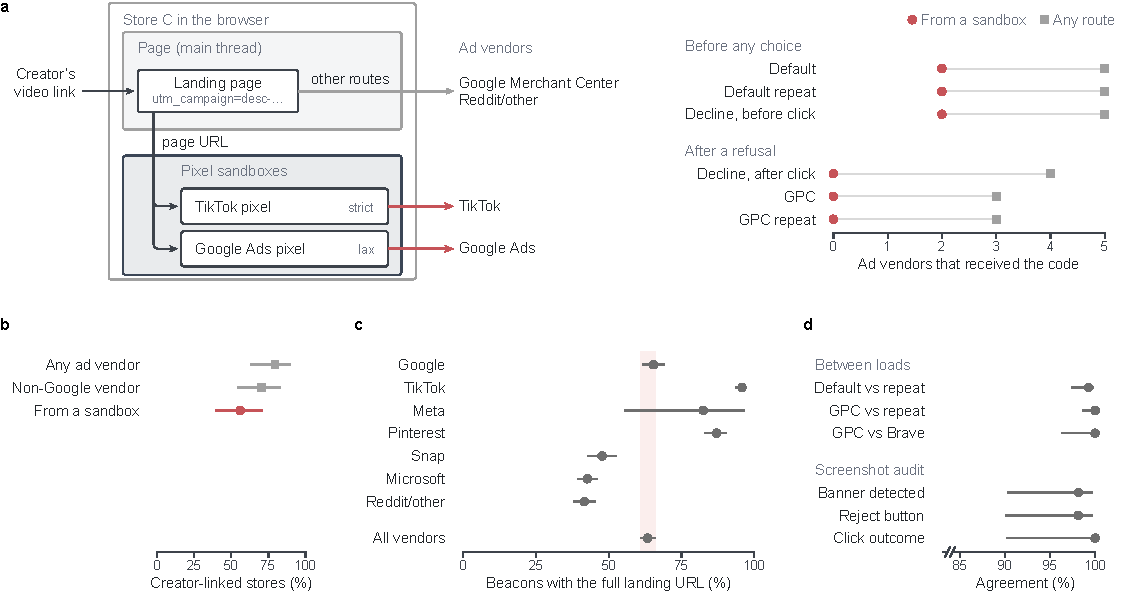
\includegraphics{fig6.pdf}
% GENERATED by paper/integrate_figures_v2.py from figures/v7/fig6/caption_fig6.tex (v2 figure caption, rendered by the figure script).
% Do not edit: change the figure script and re-run build.sh.
\caption{\textbf{Ad vendors receive the landing URL, including a creator's per-video code, and the measurements behind this repeat across loads and agree with a screenshot audit.} (a)~Store~C, a creator-linked store, loaded from a creator's video link whose uniform resource locator (URL) carries a per-video code (`utm\_campaign=desc-\ldots', the video's identifier elided here and in the drawing). Left: the code's path, on the regions of Fig.~\ref{fig:situating}a (outline: the browser; light grey ground: the page's main thread; darker grey ground: the pixel sandboxes). The landing page hands its URL to the pixels that Shopify runs in sandboxes isolated from the page, TikTok's pixel in a web worker (strict runtime) and Google Ads' pixel in a sandboxed iframe (lax runtime), and they send the code to the ad vendors outside the browser (brick arrows); scripts outside the sandboxes can send it as well (grey arrow: other routes). The ad vendors that received the code in the Default load are named at the heads of the paths that reached them. Right: one row per load of Store~C, in two groups. Before any choice: Default, its repeat, and a Decline load before the click on the banner's reject button; after a refusal: the same Decline load after the click (the rest of that page and the fresh page after the reload), a Global Privacy Control (GPC) load and its repeat (GPC refuses from the start). Brick circles: ad vendors that received the code from a sandbox; grey squares: ad vendors that received it by any route; a light line joins the two counts of a load. In each of the three loads before any choice the code reached 5 ad vendors (Google Ads, Google Merchant Center, TikTok and vendors in the Reddit/other group), 2 of them, TikTok and Google Ads, from a sandbox; TikTok's sandboxed pixel sent it in 4 requests per load. After the Decline click it still reached 4 vendors and under GPC 3, 0 of them from a sandbox, with 0 requests from TikTok's sandbox. (b)~All 34 creator-linked stores, Default load: share of stores on which the creator's code reached any ad vendor, 79.4\% (27 of 34), a vendor other than Google, 70.6\% (24 of 34), and an ad vendor from a sandbox, 55.9\% (19 of 34); Wilson 95\% confidence intervals (CIs) 63.2--89.7\%, 53.8--83.2\% and 39.5--71.1\% (horizontal lines). Marks as in (a): grey squares, by any route; brick circle, from a sandbox. (c)~Sandboxed ad beacons in the Default load that carried the full landing URL with our test code, by vendor group in a fixed order (dark grey circles; lines: Korn--Graubard 95\% CIs clustered by store): Google 65.4\% (2,689 of 4,112 beacons); TikTok 95.8\% (1,387 of 1,448); Meta 82.5\% (33 of 40); Pinterest 87.1\% (978 of 1,123); Snap 47.7\% (199 of 417); Microsoft 42.6\% (376 of 882); Reddit/other 41.7\% (1,106 of 2,654). Groups with fewer than 10 stores would be omitted; the smallest shown, Meta, has 40 beacons on 18 stores. Bottom row, set apart: all vendors, 63.4\% of 10,676 beacons on 769 stores (95\% CI 60.9--66.0\%, resampling stores); this interval is carried up through the vendor rows as a pale brick band (as the main estimates in Fig.~S5; these beacons left a sandbox before any choice), so each vendor group reads against all vendors. (d)~Robustness (dark grey circles; lines: Wilson 95\% CIs), in two named groups. The agreement axis is truncated (it does not start at zero; the break mark at its left end shows the cut); every interval ends right of the break. Between loads: agreement between two loads of the same store on whether a sandboxed ad pixel sent a request, for the validation loads, that is, repeats of Default and GPC (273 stores) and Brave's native GPC (98 stores): Default vs repeat 99.3\% (271 of 273; Cohen's $\kappa$ 0.985, 95\% CI 0.961--1.000), GPC vs repeat 100.0\% (273 of 273), emulated GPC vs Brave 100.0\% (98 of 98). Screenshot audit: the crawler's labels against saved screenshots: banner detections confirmed 98.1\% (53 of 54), first-layer reject button 98.1\% (52 of 53), click outcome 100.0\% (35 of 35). The audit labels have not yet been checked by an independent human rater. Details: Fig.~S4. In (a) and (b), brick marks the code leaving from a Shopify sandbox (consent lost) and grey marks any route. By arm, with the refusal signals that vendors receive in ad requests: Fig.~S9.
Panel~(a), left: Drawn by figure-generation scripts written with AI assistance (Section~\ref{sec:method-ai}).}
\label{fig:reach}

\end{widefig}

Some vendors register a refusal in their own layer (Supplementary Fig.~\ref*{S:fig:s9}b--c). Of Google requests of any origin, 35.6\% on the next page after a Decline and 49.3\% under GPC carried a refusal signal, as did 19.6\% and 9.6\% of Microsoft's, but almost none of the other vendors' (0.7\% under GPC). The sandboxed residuals are not explained by such signals: every remaining sandboxed request carried one on only 9 of the 53 stores with a fresh-page residual after Decline and on 18 of the 279 with a residual under GPC. Signals were read from request URLs only, so these shares are lower bounds.

\subsection{Creator links: the motivating case}\label{sec:app-creator}

On the 34 creator-linked stores, a purposive sample, the creator's code reached an ad vendor in the Default load on 27 stores, a vendor other than Google on 24, and did so from a Shopify sandbox on 19 (Fig.~\ref{fig:reach}b). Codes that name a single video reached a vendor other than Google on 3 of the 6 landing pages that carried one, so the per-video flow is not unique to \storeC, our case study (Fig.~\ref{fig:reach}a; all five loads: Supplementary Fig.~\ref*{S:fig:s9}d). On \storeC, TikTok's STRICT pixel sent the per-video code in 4 requests in each of the Default, repeat and pre-click Decline loads, and under GPC TikTok sent nothing (further detail and an edge-cache effect: Supplementary \ref*{S:sec:s-gate} and~\ref*{S:sec:s-extended}).

\subsection{Robustness and validity}\label{sec:app-validation}

\emph{Stability.} Whether a sandboxed ad request fired was stable across repeat loads (Fig.~\ref{fig:reach}d; Supplementary Fig.~\ref*{S:fig:s4}d): Default versus repeat Default agreed on 271 of 273 stores (Cohen's $\kappa=0.985$, 95\% CI 0.961--1.000) and GPC versus repeat GPC on 273 of 273. The Decline arm had no repeat load, and the timing flag repeated only moderately (Section~\ref{sec:res-prechoice}).

\emph{Emulated versus native GPC.} Brave's native GPC and our emulation agreed on whether a sandboxed ad request fired on 98 of 98 stores and 686 of 686 store--vendor pairs. Pixel code in STRICT workers read \code{navigator.globalPrivacyControl} as undefined in all 4,720 workers under emulation and 382 under Brave \citep{shopify_aboutpixels}, so on Shopify GPC acts only through Shopify's consent state and the request header, although the standard exposes it to workers \citep{w3c_gpc}.

\emph{What the pages saw of our crawler.} Every page could tell that our browser was automated: \code{navigator.webdriver} was true and the user agent contained ``HeadlessChrome'' in all 4,840 usable loads with a page probe. In the saved code of the consent tools, Pandectes' version 5 has a merchant setting, off by default according to the vendor, that for such browsers hides the banner and grants consent, which it passes to Shopify as ordinary implied consent; its signature appeared in the Default and GPC loads of 5 stores, while 31 version-5 stores configured as opt-in for California showed their banner and wrote nothing (other tools: Supplementary Table~\ref*{S:tab:s-detection}). A setting that grants consent to automated browsers makes pixels fire where a person would first see an opt-in banner, which is why the blocked-on-paper primary excludes every store whose CMP wrote ``yes''.

\emph{Sensitivity, audits and recall.} All 20 robustness variants of the three headline rates gave intervals that overlapped the main estimates (Supplementary Fig.~\ref*{S:fig:s5}), weak evidence because most variants are near-subsets of the main sample; a comparison of the six- and ten-browser crawl segments was underpowered (Supplementary \ref*{S:sec:s-sens}). In the screenshot audit of 54 seeded Decline loads, 53 detected banners were real and the reject finder agreed with the screenshots on 52 of 53, and the banner detector's recall on re-check screenshots was about 91\% (73--96\%) (Supplementary \ref*{S:sec:s-audit}). These labels are not yet an independent validation (Section~\ref{sec:method-ai}).

\subsection{Projection to the DNS frame}\label{sec:app-projection}

Weighted to the about 2,444 eligible storefronts in the DNS frame (Table~\ref{tab:projection}), about 383 stores (15.7\%, 13.5--17.9\%) show a consent banner while sending sandboxed ad requests before any choice, and with GPC switched on about 512 (20.9\%, 18.5--23.4\%) keep sending sandboxed ad requests, while at most about 7 would send them from a pixel that declares sale of data (an approximate, unweighted bound). The projections hold for the DNS frame only, whose recall is about 83\% (Section~\ref{sec:method-sample}), and no interval includes this coverage error (Supplementary \ref*{S:sec:s-extended}).

\begin{table}[!tbp]
\centering
\caption{Projection to the about 2,444 DNS-flagged storefronts in the Tranco top 200,000 (Section~\ref{sec:method-sample}), stratified by rank bucket with design weights; intervals are design-based and include the uncertainty of the frame size.}
\label{tab:projection}
\small
\tabinput{tables/table_projection.tex}%
\end{table}

% ============================================================================
\section{Discussion}\label{sec:discussion}
% ============================================================================

\subsection{Where consent is lost}\label{sec:disc-where}

Shopify's gate is not the weak point: it held back almost every configured pixel whose declared purpose had been refused, with exceptions on 7 of 1,179 stores. The interfaces around it are (Section~\ref{sec:bg-threat}). \emph{F1:} before any choice, the region default at our California vantage point allowed marketing on most stores, and sandboxed pixels fired on 70.2\% of banner stores with that default. \emph{F2:} where a blocklist declared an ad vendor blocked and the CMP had not itself consented, that vendor's pixel fired from the sandbox on 46 of 89 stores, and blocklist stores fired more often than comparable stores, because the sandbox followed Shopify's state, not the blocklist. \emph{F3:} marketing was still allowed after 20 of 231 working Decline clicks, automatic ``no'' writes arrived after 525 of 535 third-party marketing sandboxes had started, pixels started before a recorded refusal kept sending on 32 of 196 stores, and sale of data stayed allowed after 112 of the 196 refusals. \emph{F4:} pixels that declare no purpose kept sending after a recorded refusal on 28 of the 196 stores and under GPC on 191 of 1,354 and under a denying default they fired before any choice on 19 of 167 banner stores.

In security terms, the page carries two policies for the same code: the CMP's configuration states one (``TikTok: blocked'', for main-thread tags), and the platform enforces another (``allowed until the visitor declines, for the purposes the pixel declares''). The design departs from complete mediation, that every access be checked at the point that controls it \citep{saltzer1975protection}: the CMP checks tags on the main thread, but the WPM decides whether the code runs, and the WPM's own check rests on labels chosen by the party it restrains (Section~\ref{sec:bg-threat}), so a pixel that declares nothing is never checked. This gap between stated and enforced policy, of a kind security research examines elsewhere on the web \citep{latta2026policy}, follows from the architecture, not from one vendor, and may grow as more tracking moves into the sandbox \citep{shopify_checkout_upgrade}.

\subsection{Who can fix it}\label{sec:disc-fix}

\subsubsection*{Shopify}
The platform controls the only enforcement point that sees sandboxed pixels. (i) When a third-party banner is present, Shopify could hold the gate closed until the CMP has reported an initial state, as Google Consent Mode's \code{wait\_for\_update} setting does \citep{google_consentmode}, removing the race of Section~\ref{sec:res-race}. (ii) On a withdrawal of consent, the WPM could terminate the worker or remove the iframe of every pixel whose declared purpose is no longer allowed, or at least document and verifiably stop delivering events to it. (iii) Advertising apps could be required to declare the purposes their data flows serve, and merchants to declare those of custom pixels, which were involved in most residuals after a refusal; under GPC, Shopify could also hold back pixels that declare marketing, since the CCPA's opt-out covers ``sharing'' for cross-context behavioural advertising. (iv) Consent strings generated for one region should not be served to visitors from another; caching providers and merchants must keep the consent header out of cached responses.

\subsubsection*{CMP vendors}
Several vendors already document that their blockers cannot reach app or custom pixels (Section~\ref{sec:related}). They could (i) write the initial state and every choice to Shopify's Customer Privacy API by default, before the WPM's first decision; (ii) record a US Decline as a refusal of sale of data as well as marketing; (iii) show sandboxed pixels in their scanners as governed by Shopify's state, not by the blocker; (iv) offer merchants a self-test that checks, after a Decline, that no new sandbox sends ad requests; and (v) not grant consent to automated browsers, which misleads compliance scanners too.

\subsubsection*{Merchants}
A merchant who shows US visitors a banner offering a choice can make the platform consistent with it by setting the region to require consent, as almost all stores with Shopify's own banner had done, and by declaring the purposes that custom pixels serve.

\subsubsection*{Browsers and standards}
For persistence after the choice, GPC's advantage over a working Decline was at most about 10 percentage points, but GPC needs no banner integration, applies before any pixel starts, and will reach far more visitors under the 2027 browser requirement \citep{ab566,gpc_site}; it will not reach pixels that do not declare sale of data. The GPC specification exposes the signal to workers \citep{w3c_gpc}, but Shopify's STRICT sandbox hides it; preserving \code{globalPrivacyControl} inside such sandboxes would let vendor code honour it directly.

\subsection{A self-test for merchants}\label{sec:disc-tool}

Merchants cannot see these failures from their CMP's dashboard, which lists the blocked vendors, or from Shopify's, which lists the installed pixels. We therefore packaged the measurement as ConsentCheck, a command-line tool that a merchant runs against their own store: it reuses the crawler's attribution code, makes three visits with fresh profiles (Default, Decline followed by one reload, and GPC), and reports per vendor what left before any choice, from where, what the choices stopped and which blocklisted vendors the sandbox still runs, followed by the fixes of Section~\ref{sec:disc-fix} (safeguards and validation: Supplementary \ref*{S:sec:s-extended}). It is released with the code at \url{https://github.com/devanshsanghavi-droid/FTJ}.

\subsection{Legal and policy context}\label{sec:disc-law}

We make no claim that any store, CMP or platform acts unlawfully, and the measurements do not establish it; pre-choice firing is not by itself prohibited by the CCPA's opt-out rules (Section~\ref{sec:bg-law}), and we did not assess other obligations. Opt-out tools were not fully effective, mostly because of pixels whose declarations the visitor cannot see; whether those flows are a ``sale'' or ``sharing'' depends on contracts and data uses that a browser cannot observe. California enforcement has already involved opt-outs that tracking did not follow \citep{cppa2025toddsnyder,caag2025healthline,cppa2025tractorsupply}, and tracking that starts before consent has been litigated under the California Invasion of Privacy Act, including against Shopify \citep{briskin2025shopify,briskin2026remand}; SB~690, signed on 30 September 2026 (Chapter 976, Statutes of 2026) and operative from 1 January 2027, leaves suits against private actors under that act's pen-register provision over website and app tracking to the Attorney General \citep{leginfo2026sb690,duanemorris2026sb690}, and \citet{munir2025keystroke} map web tracking techniques to wiretap law (further detail: Supplementary \ref*{S:sec:s-extended}). EU visitors must consent before tracking \citep{eprivacy2002,edpb2023guidelines}; Shopify's EEA defaults may address F1 there, but our opt-in proxy (Section~\ref{sec:res-prechoice}) suggests that F4 would remain.

\subsection{Beyond Shopify}\label{sec:disc-beyond}

The blind spot is a property of any architecture that moves third-party code out of the main document: worker-offloading libraries \citep{partytown}, tag managers with their own consent layers \citep{mertens2025gtm} and server-side tagging \citep{bottger2026fpt,jazlan2026sstguard} all relocate the decision to run tracking code, and consent must then be enforced by the component that starts the code. Our pilot (Section~\ref{sec:res-beyond}) shows the consequence on other platforms: ad requests continued after a working Decline on 42\% of the Wix and 60\% of the BigCommerce sites we loaded, and first-party gateways kept collecting after refusals, although the pilot cannot say how often this happens across either platform or what a gateway forwards. For measurement the lesson is concrete: network-level crawlers see sandboxed requests but cannot tie them to the gate that started them without attribution, and audits that infer tracking from cookies \citep{bollinger2022automating,rasaii2025intractable,libert2026webxray} miss them: no ad request from a STRICT worker in the Default load carried a cookie (Supplementary \ref*{S:sec:s-extended}). Our join of declared purpose, platform consent state and container start can audit any consent-gated tag system, and we release it with our code. Automated consent audits should also report whether consent tools treat their browser as a bot.

% ============================================================================
\section{Ethics}\label{sec:ethics}
% ============================================================================

This study involved no human subjects. It measured what public storefront pages and the third-party code on them did; no person was observed, surveyed or contacted, and no personal data of real users were collected. The crawler used fresh, temporary browser profiles, never created accounts, logged in, added items to carts, submitted forms or made purchases, and interacted with consent banners only by clicking Decline or Reject, never Accept. Data flows were traced with a researcher-generated canary token. We used unmodified user agents, so our browser was visibly automated (Section~\ref{sec:app-validation}), and did not circumvent bot detection or access controls. The terms of service of individual stores were not reviewed.

\emph{\code{robots.txt}.} The Round 4 screening and crawls and ConsentCheck fetched each site's \code{robots.txt} before any other request and loaded a page only if it was allowed (Supplementary \ref*{S:sec:s-r4}). The main crawl did not consult \code{robots.txt} beforehand; a retrospective fetch found that 20 of the 1,427 stores that served one disallowed the exact landing URL we loaded, 16 only because of the campaign parameters that carried our canary (Supplementary \ref*{S:sec:s-sample}). These are the documented exceptions. Stores aimed at children or offering adult content were to be excluded, with one documented exception (Section~\ref{sec:method-sample}). After the crawl, a broader title screen found 2 adult-product stores that had been loaded, and a toy retailer and a second store that may be aimed at children were noticed; we excluded these 4 stores from all analyses for content sensitivity (Section~\ref{sec:method-sample}). Excluding in addition the 20 \code{robots.txt} cases changes no headline rate by more than 0.4 percentage points and leaves the main sample's blocked-on-paper count unchanged (Supplementary Table~\ref*{S:tab:s-ethics}).

\emph{Load on stores.} Including superseded, retried and re-check loads, each store received between 3 and 11 page loads (Supplementary \ref*{S:sec:s-sample}), at least 10.0~s apart. Most of the main crawl ran ten rather than the planned six concurrent browsers (Section~\ref{sec:method-deviations}), but each browser visited a different store, so the load on any single store did not change.

\emph{Records created by our visits.} Our visits may appear in merchants' analytics and ad-platform logs as sessions from a campaign named ``cmpstudy''; on creator links the token duplicated the creator's own campaign keys, which could affect attribution. Besides the refusals we clicked, some CMPs wrote consent states to Shopify on their own, in some cases because they detected an automated browser, and Shopify recorded a sale-of-data opt-out whenever our GPC header arrived (counts: Supplementary \ref*{S:sec:s-extended}). Future crawls should put a project-information URL in the token so that merchants can identify the study and opt out.

\emph{Reporting.} Results are reported in aggregate, and no store is named. The motivating store is called \storeC and is not named. CMP products are named where their documented capabilities determine the integration mode. The released data identify stores, and the sites of the Round 4 pilot, only by pseudonymous identifiers. This paper re-analyses pilot loads from our unpublished study of creator links, which reported the \storeC observation that motivated this one.

\emph{Disclosure.} The findings were disclosed on 2 October 2026 to Shopify, to the vendors of the three consent tools whose store-specific blocklists we evaluated (Pandectes, OneTrust and Usercentrics/Cookiebot) and to TikTok, with an invitation to correct Table~\ref{tab:cmp-modes}; the Pandectes disclosure included its merchant setting that grants consent to automated browsers. Pandectes reviewed the findings, confirmed our classification of its integration, and corrected two details of our description of its automated-browser setting (it writes no ``bot'' reason to Shopify, and the setting is off by default), which we adopted; OneTrust acknowledged receipt and asked for the store-level details, Usercentrics acknowledged receipt, and Shopify and TikTok had not replied by the time of submission.

\emph{Oversight.} No institutional review board or ethics committee determination was sought, because no human subjects were involved: the study observed no person and collected no personal data, only the behaviour of public web pages. The safeguards above (no accounts or personal data, public pages only, Decline clicks only, polite pacing, \code{robots.txt} with the documented exceptions, responsible disclosure, anonymized stores and a visibly automated browser) were applied throughout, including to the Round 4 crawls, which ran on 27 September 2026.

% ============================================================================
\section{Limitations}\label{sec:limits}
% ============================================================================

\emph{One vantage point, two days.} All loads came from one residential connection in California, on 26 September 2026 and, for Round 4, on 27 September 2026. Shopify's region defaults, and therefore the pre-choice results, differ for other US states and in particular for the EU and UK.

\emph{Visibly automated, headless browsers.} Every page could detect automation (Section~\ref{sec:app-validation}): where a consent tool grants consent to bots, pre-choice firing overstates what a person sees, and rules that hide the banner from bots lower the banner count and the detector's apparent recall, which the re-check, run with the same browser, cannot correct. Meta beacons are undercounted, and request-level sandbox shares may be higher than in a regular browser.

\emph{Declared policies.} Blocklists were readable for three CMP products. The primary blocked-on-paper estimate no longer rests on 14 stores but on 89, yet 80 of them use Pandectes, the expansion stores rank lower than the like-for-like reference, and the expansion screen stopped before its planned size (Section~\ref{sec:method-r4}). Integration modes are product-level labels, and no model can separate mode from product or default.

\emph{What we can observe.} We observed client-side requests only, so the data flows to vendors that we report are lower bounds; the store-level shares are not. A request that reached a vendor shows that data were sent, not how they were used. We never clicked Accept, the Decline arm had no repeat load, and its consent events were recorded on its last page only.

\emph{Labels, pilot and frame.} The validation labels have not yet been checked by an independent human rater (Section~\ref{sec:method-ai}). The pilot's sites were selected, not sampled, so its rates are not population estimates. The frame's recall is low in the top bucket, so the projections are conditional on the frame. Supplementary \ref*{S:sec:s-extended} gives the full list, including banner detection, the Decline procedure, timing and concurrency.

% ============================================================================
\section{Conclusion}\label{sec:conclusion}
The banner on \storeC did not govern the pixel that sent the video's code to TikTok; we measured how often and where such gaps open across 1,358 popular storefronts and 116 lower-ranked ones from California. Where a blocklist declared an ad vendor blocked and the consent tool had not itself consented, that vendor's pixel fired from Shopify's sandbox before any choice on 46 of 89 stores: sandboxed pixels followed Shopify's consent state, not the blocklist. Shopify's gate held back almost every pixel declaring a refused purpose, but its California default allowed tracking on most stores, automatic refusals came late, and pixels that started earlier or declared other purposes or none kept sending: after a working Decline, a new sandbox still sent ad requests on 23\% of stores, and GPC by design stopped only pixels declaring sale of data. A pilot on selected non-Shopify sites found ad requests after refusals too. The repair needs no new law: Shopify can hold its gate until the consent tool reports and stop pixels on withdrawal, consent tools can report every choice, and merchants can require consent and test their stores with ConsentCheck. Consent must be enforced by the component that starts the code.


% backmatter.tex -- declarations required by Computers & Security / Elsevier (shared by both builds).
% Order follows the Elsevier guide: declarations, then the generative-AI declaration immediately before the references.
% Finalized for a sole author on 2026-09-28; author details, data link, AI declaration and biography filled in on
% 2026-09-29. No placeholder or \todo remains, so the strict build compiles.

\section*{Ethics statement}
This study involved no human subjects: it measured the behaviour of public web pages and the third-party code on them, observed no person and collected no personal data of real users. No institutional review board or ethics committee determination was sought, for the reasons and with the safeguards given in Section~\ref{sec:ethics}, which also describes the responsible disclosure made before submission.

\section*{Data and code availability}
The crawler and its configuration (CMP signatures, vendor endpoint map, Web Pixels URL patterns), the analysis scripts (including the gate audit, which joins declared purposes, Shopify's consent state and container starts), ConsentCheck, the figure code and the aggregate outputs are available at \url{https://github.com/devanshsanghavi-droid/FTJ}. One script regenerates the analysis outputs, every data figure and almost every number in this paper from the saved crawl data; the few remaining numbers (from the crawl log, pilot notes and literature) are traced to their saved sources by an automated check. The store sample (Tranco rank bucket, Shopify verification markers and design weights), the request-level data (vendor, origin, timing and payload flags; hosts only, no full URLs; canary tokens only, no user data), the consent-state readings, the re-check results, the \code{robots.txt} and frame-recall summaries, and the text part of a kit for blind re-labelling of every validation label are released with pseudonymous store identifiers. Screenshots (which show store names), raw browser captures (which may contain third-party cookies set during crawling, and which include the re-check's script-element logs) and the mapping to domains are available to researchers on request, and merchants can ask for their store's records to be removed, from the author (devansh.sanghavi@gmail.com).

\section*{CRediT authorship contribution statement}
\textbf{Devansh Sanghavi:} Conceptualization, Methodology, Software, Validation, Formal analysis, Investigation, Data curation, Visualization, Project administration, Writing -- original draft, Writing -- review \& editing.

\section*{Declaration of competing interest}
The author declares that they have no known competing financial interests or personal relationships that could have appeared to influence the work reported in this paper.

\section*{Funding}
This research did not receive any specific grant from funding agencies in the public, commercial, or not-for-profit sectors.

\section*{Declaration of generative AI and AI-assisted technologies in the manuscript preparation process}
During the preparation of this work the author used Anthropic's Claude to assist with writing and debugging the measurement, analysis, and figure-generation scripts. The author reviewed the code and its outputs and takes full responsibility for the content of the publication.

\bibliographystyle{elsarticle-harv}
\bibliography{refs}

% ---- Author biography (Elsevier: 50-100 words per author for full-length articles) ----
\section*{Author biography}
\noindent\textbf{Devansh Sanghavi} is a junior at Los Altos High School in Los Altos, California, USA. His research interests are web privacy measurement and the evaluation of AI systems. For this study he designed and ran a large-scale web measurement with Playwright browser automation, and analysed the data in Python with pandas and statsmodels, including cluster-bootstrap confidence intervals. He is a research intern at Paper Lantern, surveying benchmarks and environments for evaluating AI models, and builds civic-technology apps with security features such as field-level encryption. He also competes in mathematics and robotics.

\end{document}
